% A LaTeX template fitted for a Phd thesis report
% Copyright (C) 2013 Damien Roque

% This program is free software; you can redistribute it and/or
% modify it under the terms of the GNU General Public License
% as published by the Free Software Foundation; either version 2
% of the License, or (at your option) any later version.

% This program is distributed in the hope that it will be useful,
% but WITHOUT ANY WARRANTY; without even the implied warranty of
% MERCHANTABILITY or FITNESS FOR A PARTICULAR PURPOSE.  See the
% GNU General Public License for more details.

% You should have received a copy of the GNU General Public License
% along with this program; if not, write to the Free Software
% Foundation, Inc., 51 Franklin Street, Fifth Floor, Boston, MA  02110-1301, USA.

% Author : Damien Roque <damien.roque@gipsa-lab.grenoble-inp.fr>

\documentclass[a4paper,11pt,twoside]{templates/roque-phdthesis-template}

% Include configuration (loading packages, defining the style of the document...)
\usepackage[utf8]{inputenc}
\RequirePackage[l2tabu, orthodox]{nag} % check all packages

\usepackage[a4paper]{templates/first-page-udg}

% Encoding and internationalization
\usepackage[T1]{fontenc}
\usepackage{aecompl}
\usepackage[utf8]{inputenc}  % For accent
% \usepackage[french]{babel} % Comment this line if the document is written in english
\usepackage[american]{babel} % Comment this line if the document is written in english

% Math packages
\usepackage{amsmath,amssymb}
\usepackage{mathrsfs}
\usepackage{amsthm}
\usepackage{a4wide}
\renewcommand{\baselinestretch}{1.05}

% Mini table of content and acronyms
\usepackage[nottoc, notlof, notlot]{tocbibind}
\usepackage[french]{minitoc}
\setcounter{minitocdepth}{2}
\mtcindent=15pt
\setlength{\parskip}{10pt}

\let\minitocORIG\minitoc
\renewcommand{\minitoc}{\minitocORIG \vspace{1.5em}}

\setcounter{secnumdepth}{3}
\setcounter{tocdepth}{2}

% Graphics and hyperlinks
\usepackage{ifpdf}
\ifpdf
  \usepackage[pdftex]{graphicx}
  \DeclareGraphicsExtensions{.jpg,.pdf,.png}
  %\usepackage[a4paper,pagebackref,hyperindex=true]{hyperref}
  \usepackage[a4paper,hyperindex=true]{hyperref}
\else
  \usepackage{graphicx}
  \DeclareGraphicsExtensions{.ps,.eps}
  %\usepackage[a4paper,dvipdfm,pagebackref,hyperindex=true]{hyperref}
  \usepackage[a4paper,dvipdfm,hyperindex=true]{hyperref}
\fi
\graphicspath{{.}{images/}}
\usepackage{eso-pic}
\usepackage{rotating}
\usepackage[font=normalsize]{subfig}
\usepackage{tikz}
\usetikzlibrary{shapes,arrows}
\usepackage{pgfplots}
\pgfplotsset{compat=newest}
\pgfplotsset{plot coordinates/math parser=false}
\newlength\figureheight
\newlength\figurewidth

\pgfkeys{/pgf/number format/.cd,
set decimal separator={,\!},
1000 sep={\,},
} % Comment this line if the document is written in english

\usetikzlibrary{plotmarks}
\usepackage{pdfpages}

\usepackage[strict]{changepage}
\newcommand\BackgroundPic{
\put(0,0){
\parbox[b][\paperheight]{\paperwidth}{%
\vfill
\centering

\includegraphics[width=0.9\paperwidth,height=1\paperheight,keepaspectratio]{images/background-eps-converted-to}%
\vfill
}}}

\usepackage{color}
\definecolor{linkcol}{rgb}{0,0,0} 
\definecolor{citecol}{rgb}{0,0,0}

\hypersetup
{
bookmarksopen=true,
pdftitle={Mon sujet de thèse complet},
pdfauthor={Prénom NOM},
pdfsubject={Rapport de thèse},
pdfmenubar=true,
pdfhighlight=/O,
colorlinks=true,
pdfpagemode=None,
pdfpagelayout=SinglePage,
pdffitwindow=true,
linkcolor=linkcol,
citecolor=citecol,
urlcolor=linkcol
}



% Headers and footers
\usepackage{fancyhdr}
\pagestyle{fancy}
\fancyfoot{}
\fancyhead[LE,RO]{\bfseries\thepage}
\fancyhead[RE]{\bfseries\nouppercase{\leftmark}}
\fancyhead[LO]{\bfseries\nouppercase{\rightmark}}

\let\headruleORIG\headrule
\renewcommand{\headrule}{\color{black} \headruleORIG}
\renewcommand{\headrulewidth}{1.0pt}
\usepackage{colortbl}
\arrayrulecolor{black}

\fancypagestyle{plain}{
  \fancyhead{}
  \fancyfoot[C]{\thepage}
  \renewcommand{\headrulewidth}{0pt}
}

\usepackage[footnote]{acronym}

% References formatting
% Bibtex
% \renewcommand*{\backref}[1]{}
% \renewcommand*{\backrefalt}[4]{%
% \ifcase #1 %
% (Non cité.)%
% \or
% (Cité en page~#2.)%
% \else
% (Cité en pages~#2.)%
% \fi}
% \renewcommand*{\backrefsep}{, }
% \renewcommand*{\backreftwosep}{ et~}
% \renewcommand*{\backreflastsep}{ et~}

% BibLatex
\usepackage[style=alphabetic-verb,backend=bibtex,isbn=false,doi=false,backref=true,url=false]{biblatex}
\addbibresource{references.bib}

% Pages succession
\makeatletter
\def\cleardoublepage{\clearpage\if@twoside \ifodd\c@page\else%
  \hbox{}%
  \thispagestyle{empty}%
  \newpage%
  \if@twocolumn\hbox{}\newpage\fi\fi\fi}
\makeatother

\newenvironment{vcenterpage}
{\newpage\vspace*{\fill}\thispagestyle{empty}\renewcommand{\headrulewidth}{0pt}}
{\vspace*{\fill}}

%%% Local Variables: 
%%% mode: latex
%%% TeX-master: "../roque-phdthesis"
%%% End: 


%% TO DO
\usepackage{titlesec}
\titleclass{\part}{top}
\titleformat{\part}[display]
{\normalfont\huge\bfseries}{\centering\partname\ \thepart}{20pt}{\Huge\centering}
\titlespacing*{\part}{0pt}{50pt}{40pt}
%\titleclass{\chapter}{straight}
%\titleformat{\chapter}[display]
%{\normalfont\huge\bfseries}{\chaptertitlename\ \thechapter}{20pt}{\Huge}
%\titlespacing*{\chapter} {0pt}{50pt}{40pt}


\usepackage{amsmath,amsfonts}

% Top 9 packages
% \usepackage{microtype}
% The microtype package improves the spacing between words and letters. It does a lot more and most people won’t notice the difference. But still, the resulting document will be easier to read and looks better when microtype is loaded. Load this package after fonts, if any, as the package behavior is dependent on this font. - See more at: http://www.howtotex.com/packages/9-essential-latex-packages-everyone-should-use/#sthash.e5Qsr4ay.dpuf
% \usepackage{siunitx}
% The siunitx package greatly simplifies TeXing when writing scientific documents, where units and numbers are a big part of the writing. This package adds commands like \num for typesetting numbers in all sorts of ways and \si for units. The commands I use a lot are \SI and \SIrange. For example, \SI{10}{\hertz} results in ‘10Hz‘ in text (this is especially useful to prevent typo’s; I tend to write HZ or hz a lot instead of Hz). The \SIrange command requires one more input variable: \SIrange{10}{100}{\hertz} produces ‘10Hz to 100Hz‘. Note that the siunitx package was already featured in an earlier post on this blog. - See more at: http://www.howtotex.com/packages/9-essential-latex-packages-everyone-should-use/#sthash.e5Qsr4ay.dpuf
% \usepackage{cleveref}
% Another fascinating LaTeX package is cleveref. This package introduces the \cref command. When using this command to make cross-references, instead of \ref or \eqref, a word is placed in front of the reference according to the type of reference: fig. for figures, eq. for equations. Hence, another LaTeX package that simplifies the writing. The package was earlier mentioned in this post. In that post it is also shown how to change the words in front of references. - See more at: http://www.howtotex.com/packages/9-essential-latex-packages-everyone-should-use/#sthash.e5Qsr4ay.dpuf
% \usepackage[colorlinks=false, pdfborder={0 0 0}]{hyperref} 
% See more at: http://www.howtotex.com/packages/9-essential-latex-packages-everyone-should-use/#sthash.e5Qsr4ay.dpuf
% \usepackage{booktabs}
% The booktabs package allows you to create tables without vertical separators. These separators are just unnecessary and plain ugly. Creating a table with booktabs is however more of a pain than the normal way of creating LaTeX tables. Therefore, I dedicated a post on how to create nice tables with the booktabs package earlier. - See more at: http://www.howtotex.com/packages/9-essential-latex-packages-everyone-should-use/#sthash.e5Qsr4ay.dpuf
\usepackage{todonotes}



%\usepackage{hyperref}
%\hypersetup{bookmarks,bookmarksopen,bookmarksdepth=2}

% Include user's macros
% Math macros
\newcommand*{\SET}[1]  {\ensuremath{\mathrm{\mathbf{#1}}}}
\newcommand*{\VEC}[1]  {\ensuremath{\boldsymbol{#1}}}
\newcommand*{\MAT}[1]  {\ensuremath{\boldsymbol{#1}}}
\newcommand*{\OP}[1]  {\ensuremath{\boldsymbol{\mathcal{#1}}}}
\newcommand*{\ESP}[1]  {\ensuremath{ \mathbb{E} \left \{#1 \right \}}}
\newcommand*{\ESPENS}[2]  {\ensuremath{ \mathbb{E}_{#1} \left \{#2 \right \}}}
\newcommand*{\NORM}[1]  {\ensuremath{\left\|#1\right\|}}
\newcommand*{\DPR}[2]  {\ensuremath{\left \langle #1,#2 \right \rangle}}
\newcommand*{\FOURIER}[1]  {\ensuremath{\widehat{#1}}}
\newcommand{\eqdef}{\stackrel{\mathrm{def}}{=}}
\newcommand{\argmax}{\operatornamewithlimits{argmax}}
\newcommand{\argmin}{\operatornamewithlimits{argmin}}
\newcommand{\diag}{\operatorname{diag}}
\newcommand{\ud}{\, \mathrm{d}}
\newcommand{\vect}{\mathrm{Vect}}
\newcommand{\sinc}{\mathrm{sinc}}
\newcommand{\esp}{\ensuremath{\mathrm{E}}} % Problème pour les short captions
\newcommand{\hilbert}{\ensuremath{\mathcal{H}}}
\newcommand{\supps}{\ensuremath{\tilde{\mathrm{supp}}}}
\newcommand{\supp}{\ensuremath{\mathrm{supp}}}
\newcommand{\sgn}{\mathrm{sgn}}
\newcommand{\intTT}{\int_{-T}^{T}}
\newcommand{\intT}{\int_{-\frac{T}{2}}^{\frac{T}{2}}}
\newcommand{\intinf}{\int_{-\infty}^{+\infty}}
\newcommand{\iintinf}{\iint_{-\infty}^{+\infty}}
\newcommand{\iintrr}{\iint\limits_{\SET{R}^2}}
\newcommand{\intr}{\int\limits_{\R}}
\newcommand{\Sh}{\ensuremath{\boldsymbol{U}}}
\newcommand{\C}{\ensuremath{\mathbf{C}}}
\newcommand{\R}{\ensuremath{\mathbf{R}}}
\newcommand{\Z}{\ensuremath{\mathbf{Z}}}
\newcommand{\N}{\ensuremath{\mathbf{N}}}
\newcommand{\K}{\ensuremath{\mathbf{K}}}
\newcommand{\reel}{\mathcal{R}}
\newcommand{\imag}{\mathcal{I}}
\newcommand{\cmnr}{c_{m,n}^\reel}
\newcommand{\cmni}{c_{m,n}^\imag}
\newcommand{\cnr}{c_{n}^\reel}
\newcommand{\cni}{c_{n}^\imag}
\newcommand{\tproto}{g}
\newcommand{\rproto}{\check{g}}
\newcommand{\Tproto}{G}
\newcommand{\Rproto}{\check{G}}
\newcommand{\Tpoly}{F}
\newcommand{\Rpoly}{\check{F}}
\newcommand{\estim}{\tilde{c}}
\newcommand{\egal}{\bar{c}}
\newcommand{\bb}{b}
\newcommand{\bbf}{z}
\newcommand{\bbr}{\zeta}
\newcommand{\LR}{\mathcal{L}_2(\R)}
\newcommand{\LRR}{\mathcal{L}_2(\R^2)}
\newcommand{\LZ}{\ell_2(\Z)}
\newcommand{\LZZ}{\ell_2(\Z^2)}
\newcommand{\peigne}{\ensuremath{\Psi}}
\newcommand{\avec}{\qquad \text{avec} \qquad}

% Theorems definition
\newtheoremstyle{break}
  {11pt}{11pt}%
  {\itshape}{}%
  {\bfseries}{}%
  {\newline}{}%
\theoremstyle{break}

\newtheorem{definition}{Définition}[chapter]
\newtheorem{theoreme}{Théorème}[chapter]
\newtheorem{remarque}{Remarque}[chapter]
\newtheorem{propriete}{Propriété}[chapter]
\newtheorem{exemple}{Exemple}[chapter]

% Example of background tag
% \AddToShipoutPicture{%
% \begin{tikzpicture}[remember picture,overlay]
%   \node [rotate=60,scale=10,text opacity=0.1] at (current page.center) {Brouillon};
% \end{tikzpicture}}

% Example of header tag
% \AddToShipoutPicture{%
% \tikzstyle{block} = [draw, thick, color=blue, scale=1.5,rectangle, minimum height=3em, minimum width=6em]
% \begin{tikzpicture}[remember picture,overlay]
%   \node [coordinate] at (current page.north) (accroche) {};
%   \node [block, below of=accroche] {Diffusion restreinte};
% \end{tikzpicture}}

% Another example of header tag
% \AddToShipoutPicture{%
% \tikzstyle{block} = [draw, thick, color=red, scale=1.5,rectangle, minimum height=3em, minimum width=6em]
% \begin{tikzpicture}[remember picture,overlay]
%   \node [coordinate] at (current page.north) (accroche) {};
%   \node [block, below of=accroche] {Confidentiel Défense};
% \end{tikzpicture}}

%%% Local Variables: 
%%% mode: latex
%%% TeX-master: "../roque-phdthesis"
%%% End: 

% Build only the following parts of the document (recommended for large documents)
% \chapter*{Introduction}
\addstarredchapter{Introduction}
\markboth{Introduction}{Introduction}
\label{chap:introduction}
%\minitoc

Lorem ipsum dolor sit amet, consectetur adipiscing elit. Sed non risus. Suspendisse lectus tortor, dignissim sit amet, adipiscing nec, ultricies sed, dolor. Cras elementum ultrices diam. Maecenas ligula massa, varius a, semper congue, euismod non, mi. Proin porttitor, orci nec nonummy molestie, enim est eleifend mi, non fermentum diam nisl sit amet erat. Duis semper. Duis arcu massa, scelerisque vitae, consequat in, pretium a, enim. Pellentesque congue. Ut in risus volutpat libero pharetra tempor. Cras vestibulum bibendum augue. Praesent egestas leo in pede. Praesent blandit odio eu enim. Pellentesque sed dui ut augue blandit sodales. Vestibulum ante ipsum primis in faucibus orci luctus et ultrices posuere cubilia Curae; Aliquam nibh. Mauris ac mauris sed pede pellentesque fermentum. Maecenas adipiscing ante non diam sodales hendrerit. Ut velit mauris, egestas sed, gravida nec, ornare ut, mi. Aenean ut orci vel massa suscipit pulvinar. Nulla sollicitudin. Fusce varius, ligula non tempus aliquam, nunc turpis ullamcorper nibh, in tempus sapien eros vitae ligula. Pellentesque rhoncus nunc et augue. Integer id felis. Curabitur aliquet pellentesque diam. Integer quis metus vitae elit lobortis egestas. Lorem ipsum dolor sit amet, consectetuer adipiscing elit. Morbi vel erat non mauris convallis vehicula. Nulla et sapien. Integer tortor tellus, aliquam faucibus, convallis id, congue eu, quam. Mauris ullamcorper felis vitae erat. Proin feugiat, augue non elementum posuere, metus purus iaculis lectus, et tristique ligula justo vitae magna. Aliquam convallis sollicitudin purus. Praesent aliquam, enim at fermentum mollis, ligula massa adipiscing nisl, ac euismod nibh nisl eu lectus. Fusce vulputate sem at sapien. Vivamus leo. Aliquam euismod libero eu enim. Nulla nec felis sed leo placerat imperdiet. Aenean suscipit nulla in justo. Suspendisse cursus rutrum augue. Nulla tincidunt tincidunt mi. Curabitur iaculis, lorem vel rhoncus faucibus, felis magna fermentum augue, et ultricies lacus lorem varius purus. Curabitur eu amet.

Lorem ipsum dolor sit amet, consectetur adipiscing elit. Sed non risus. Suspendisse lectus tortor, dignissim sit amet, adipiscing nec, ultricies sed, dolor. Cras elementum ultrices diam. Maecenas ligula massa, varius a, semper congue, euismod non, mi. Proin porttitor, orci nec nonummy molestie, enim est eleifend mi, non fermentum diam nisl sit amet erat. Duis semper. Duis arcu massa, scelerisque vitae, consequat in, pretium a, enim. Pellentesque congue. Ut in risus volutpat libero pharetra tempor. Cras vestibulum bibendum augue. Praesent egestas leo in pede. Praesent blandit odio eu enim. Pellentesque sed dui ut augue blandit sodales. Vestibulum ante ipsum primis in faucibus orci luctus et ultrices posuere cubilia Curae; Aliquam nibh. Mauris ac mauris sed pede pellentesque fermentum. Maecenas adipiscing ante non diam sodales hendrerit. Ut velit mauris, egestas sed, gravida nec, ornare ut, mi. Aenean ut orci vel massa suscipit pulvinar. Nulla sollicitudin. Fusce varius, ligula non tempus aliquam, nunc turpis ullamcorper nibh, in tempus sapien eros vitae ligula. Pellentesque rhoncus nunc et augue. Integer id felis. Curabitur aliquet pellentesque diam. Integer quis metus vitae elit lobortis egestas. Lorem ipsum dolor sit amet, consectetuer adipiscing elit. Morbi vel erat non mauris convallis vehicula. Nulla et sapien. Integer tortor tellus, aliquam faucibus, convallis id, congue eu, quam. Mauris ullamcorper felis vitae erat. Proin feugiat, augue non elementum posuere, metus purus iaculis lectus, et tristique ligula justo vitae magna. Aliquam convallis sollicitudin purus. Praesent aliquam, enim at fermentum mollis, ligula massa adipiscing nisl, ac euismod nibh nisl eu lectus. Fusce vulputate sem at sapien. Vivamus leo. Aliquam euismod libero eu enim. Nulla nec felis sed leo placerat imperdiet. Aenean suscipit nulla in justo. Suspendisse cursus rutrum augue. Nulla tincidunt tincidunt mi. Curabitur iaculis, lorem vel rhoncus faucibus, felis magna fermentum augue, et ultricies lacus lorem varius purus. Curabitur eu amet.

Lorem ipsum dolor sit amet, consectetur adipiscing elit. Sed non risus. Suspendisse lectus tortor, dignissim sit amet, adipiscing nec, ultricies sed, dolor. Cras elementum ultrices diam. Maecenas ligula massa, varius a, semper congue, euismod non, mi. Proin porttitor, orci nec nonummy molestie, enim est eleifend mi, non fermentum diam nisl sit amet erat. Duis semper. Duis arcu massa, scelerisque vitae, consequat in, pretium a, enim. Pellentesque congue. Ut in risus volutpat libero pharetra tempor. Cras vestibulum bibendum augue. Praesent egestas leo in pede. Praesent blandit odio eu enim. Pellentesque sed dui ut augue blandit sodales. Vestibulum ante ipsum primis in faucibus orci luctus et ultrices posuere cubilia Curae; Aliquam nibh. Mauris ac mauris sed pede pellentesque fermentum. Maecenas adipiscing ante non diam sodales hendrerit. Ut velit mauris, egestas sed, gravida nec, ornare ut, mi. Aenean ut orci vel massa suscipit pulvinar. Nulla sollicitudin. Fusce varius, ligula non tempus aliquam, nunc turpis ullamcorper nibh, in tempus sapien eros vitae ligula. Pellentesque rhoncus nunc et augue. Integer id felis. Curabitur aliquet pellentesque diam. Integer quis metus vitae elit lobortis egestas. Lorem ipsum dolor sit amet, consectetuer adipiscing elit. Morbi vel erat non mauris convallis vehicula. Nulla et sapien. Integer tortor tellus, aliquam faucibus, convallis id, congue eu, quam. Mauris ullamcorper felis vitae erat. Proin feugiat, augue non elementum posuere, metus purus iaculis lectus, et tristique ligula justo vitae magna. Aliquam convallis sollicitudin purus. Praesent aliquam, enim at fermentum mollis, ligula massa adipiscing nisl, ac euismod nibh nisl eu lectus. Fusce vulputate sem at sapien. Vivamus leo. Aliquam euismod libero eu enim. Nulla nec felis sed leo placerat imperdiet. Aenean suscipit nulla in justo. Suspendisse cursus rutrum augue. Nulla tincidunt tincidunt mi. Curabitur iaculis, lorem vel rhoncus faucibus, felis magna fermentum augue, et ultricies lacus lorem varius purus. Curabitur eu amet.


% \chapter{Premier chapitre}
\label{chap:premierchapitre}
\minitoc

\section{Une section}
Lorem ipsum dolor sit amet, consectetur adipiscing elit \cite{Roque2012,Roque2012b,Roque2012c,Roque2012d}. Sed non risus \cite{Bello1963}. Suspendisse lectus tortor, dignissim sit amet, adipiscing nec, ultricies sed, dolor. Cras elementum ultrices diam. Maecenas ligula massa, varius a, semper congue, euismod non, mi. Proin porttitor, orci nec nonummy molestie, enim est eleifend mi, non fermentum diam nisl sit amet erat. Duis semper. Duis arcu massa, scelerisque vitae, consequat in, pretium a, enim. Pellentesque congue. Ut in risus volutpat libero pharetra tempor. Cras vestibulum bibendum augue. Praesent egestas leo in pede. Praesent blandit odio eu enim. Pellentesque sed dui ut augue blandit sodales. Vestibulum ante ipsum primis in faucibus orci luctus et ultrices posuere cubilia Curae; Aliquam nibh. Mauris ac mauris sed pede pellentesque fermentum. Maecenas adipiscing ante non diam sodales hendrerit. Ut velit mauris, egestas sed, gravida nec, ornare ut, mi. Aenean ut orci vel massa suscipit pulvinar. Nulla sollicitudin. Fusce varius, ligula non tempus aliquam, nunc turpis ullamcorper nibh, in tempus sapien eros vitae ligula. Pellentesque rhoncus nunc et augue. Integer id felis. Curabitur aliquet pellentesque diam. Integer quis metus vitae elit lobortis egestas. Lorem ipsum dolor sit amet, consectetuer adipiscing elit. Morbi vel erat non mauris convallis vehicula. Nulla et sapien. Integer tortor tellus, aliquam faucibus, convallis id, congue eu, quam. Mauris ullamcorper felis vitae erat. Proin feugiat, augue non elementum posuere, metus purus iaculis lectus, et tristique ligula justo vitae magna. Aliquam convallis sollicitudin purus. Praesent aliquam, enim at fermentum mollis, ligula massa adipiscing nisl, ac euismod nibh nisl eu lectus. Fusce vulputate sem at sapien. Vivamus leo. Aliquam euismod libero eu enim. Nulla nec felis sed leo placerat imperdiet. Aenean suscipit nulla in justo. Suspendisse cursus rutrum augue. Nulla tincidunt tincidunt mi. Curabitur iaculis, lorem vel rhoncus faucibus, felis magna fermentum augue, et ultricies lacus lorem varius purus. Curabitur eu amet (fig. \ref{fig:une-image}).

\begin{figure}[htp]
  \centering
  \tikzstyle{block} = [draw, fill=blue!20, rectangle, minimum height=3em, minimum width=6em, text width=6em,text centered]
\begin{tikzpicture}[auto, node distance=3.5cm,>=latex']
\shorthandoff{:} % Evite le bug de compilation avec tikz
    % Longueurs et espacement
    \def\longabove{0.2cm}
    \def\espacement{4cm}

    % Définition des blocs
    \node [block, node distance=\espacement] (codeur) {Codeur};
    \node [block, right of=codeur, node distance=\espacement] (cbs) {Conversion bits/symboles};
    \node [block, right of=cbs, node distance=\espacement] (modulateur) {Modulateur};
 
    % Définition des liens
    \draw [<-] (codeur) -- ++(-2,0) node[left] {$\{b_n\}$};
    \draw [->] (codeur) -- node[above=\longabove] {$\{d_n\}$} (cbs);
    \draw [->] (cbs) -- node[above=\longabove] {$\{c_k\}$} (modulateur);
    \draw [->] (modulateur) -- ++(2,0) node[right] {$s(t)$};
\end{tikzpicture}

  \caption{Exemple de diagramme TikZ.}
  \label{fig:une-image}
\end{figure}

\section{Une autre section}
Lorem ipsum dolor sit amet, consectetur adipiscing elit. Sed non risus. Suspendisse lectus tortor, dignissim sit amet, adipiscing nec, ultricies sed, dolor. Cras elementum ultrices diam. Maecenas ligula massa, varius a, semper congue, euismod non, mi. Proin porttitor, orci nec nonummy molestie, enim est eleifend mi, non fermentum diam nisl sit amet erat. Duis semper. Duis arcu massa, scelerisque vitae, consequat in, pretium a, enim. Pellentesque congue. Ut in risus volutpat libero pharetra tempor. Cras vestibulum bibendum augue. Praesent egestas leo in pede. Praesent blandit odio eu enim. Pellentesque sed dui ut augue blandit sodales. Vestibulum ante ipsum primis in faucibus orci luctus et ultrices posuere cubilia Curae; Aliquam nibh. Mauris ac mauris sed pede pellentesque fermentum. Maecenas adipiscing ante non diam sodales hendrerit. Ut velit mauris, egestas sed, gravida nec, ornare ut, mi. Aenean ut orci vel massa suscipit pulvinar. Nulla sollicitudin. Fusce varius, ligula non tempus aliquam, nunc turpis ullamcorper nibh, in tempus sapien eros vitae ligula. Pellentesque rhoncus nunc et augue. Integer id felis. Curabitur aliquet pellentesque diam. Integer quis metus vitae elit lobortis egestas. Lorem ipsum dolor sit amet, consectetuer adipiscing elit. Morbi vel erat non mauris convallis vehicula. Nulla et sapien. Integer tortor tellus, aliquam faucibus, convallis id, congue eu, quam. Mauris ullamcorper felis vitae erat. Proin feugiat, augue non elementum posuere, metus purus iaculis lectus, et tristique ligula justo vitae magna. Aliquam convallis sollicitudin purus. Praesent aliquam, enim at fermentum mollis, ligula massa adipiscing nisl, ac euismod nibh nisl eu lectus. Fusce vulputate sem at sapien. Vivamus leo. Aliquam euismod libero eu enim. Nulla nec felis sed leo placerat imperdiet. Aenean suscipit nulla in justo. Suspendisse cursus rutrum augue. Nulla tincidunt tincidunt mi. Curabitur iaculis, lorem vel rhoncus faucibus, felis magna fermentum augue, et ultricies lacus lorem varius purus. Curabitur eu amet (tab. \ref{tab:un-tableau}).

\begin{table}[ht]
  \begin{center}
    \begin{tabular}{|c|c|c|c|c|}
      \hline
      & $h(t,\tau)$ & $S_{\OP{H}}^{(\alpha)} (f,\tau)$ & $L_{\OP{H}}^{(\alpha)} (\nu,t)$ & $H^{(\alpha)}(f,\nu)$ \\
      \hline
      LTI & $q(\tau)$ & $q(\tau) \delta(f)$ & $Q(\nu)$ & $Q(\nu) \delta(\nu-f)$ \\
      \hline
      LFI & $m(t) \delta(\tau)$ & $M(f) \delta(\tau)$ & $m(t)$ & $M(f)$\\
      \hline
      identité & $\delta(t)$ & $\delta(f)\delta(\tau)$ & $1$ & $\delta(\nu-f)$\\
      \hline
    \end{tabular}
    \caption{Exemple de tableau.}
    \label{tab:un-tableau}
  \end{center}
\end{table}

Lorem ipsum dolor sit amet, consectetur adipiscing elit. Sed non risus. Suspendisse lectus tortor, dignissim sit amet, adipiscing nec, ultricies sed, dolor. Cras elementum ultrices diam. Maecenas ligula massa, varius a, semper congue, euismod non, mi. Proin porttitor, orci nec nonummy molestie, enim est eleifend mi, non fermentum diam nisl sit amet erat. Duis semper. Duis arcu massa, scelerisque vitae, consequat in, pretium a, enim. Pellentesque congue. Ut in risus volutpat libero pharetra tempor. Cras vestibulum bibendum augue. Praesent egestas leo in pede. Praesent blandit odio eu enim. Pellentesque sed dui ut augue blandit sodales. Vestibulum ante ipsum primis in faucibus orci luctus et ultrices posuere cubilia Curae; Aliquam nibh. Mauris ac mauris sed pede pellentesque fermentum. Maecenas adipiscing ante non diam sodales hendrerit. Ut velit mauris, egestas sed, gravida nec, ornare ut, mi. Aenean ut orci vel massa suscipit pulvinar. Nulla sollicitudin. Fusce varius, ligula non tempus aliquam, nunc turpis ullamcorper nibh, in tempus sapien eros vitae ligula. Pellentesque rhoncus nunc et augue. Integer id felis. Curabitur aliquet pellentesque diam. Integer quis metus vitae elit lobortis egestas. Lorem ipsum dolor sit amet, consectetuer adipiscing elit. Morbi vel erat non mauris convallis vehicula. Nulla et sapien. Integer tortor tellus, aliquam faucibus, convallis id, congue eu, quam. Mauris ullamcorper felis vitae erat. Proin feugiat, augue non elementum posuere, metus purus iaculis lectus, et tristique ligula justo vitae magna. Aliquam convallis sollicitudin purus. Praesent aliquam, enim at fermentum mollis, ligula massa adipiscing nisl, ac euismod nibh nisl eu lectus. Fusce vulputate sem at sapien. Vivamus leo. Aliquam euismod libero eu enim. Nulla nec felis sed leo placerat imperdiet. Aenean suscipit nulla in justo. Suspendisse cursus rutrum augue. Nulla tincidunt tincidunt mi. Curabitur iaculis, lorem vel rhoncus faucibus, felis magna fermentum augue, et ultricies lacus lorem varius purus. Curabitur eu amet (fig. \ref{fig:une-autre-image}).

\begin{figure}[htp]
  \centering
  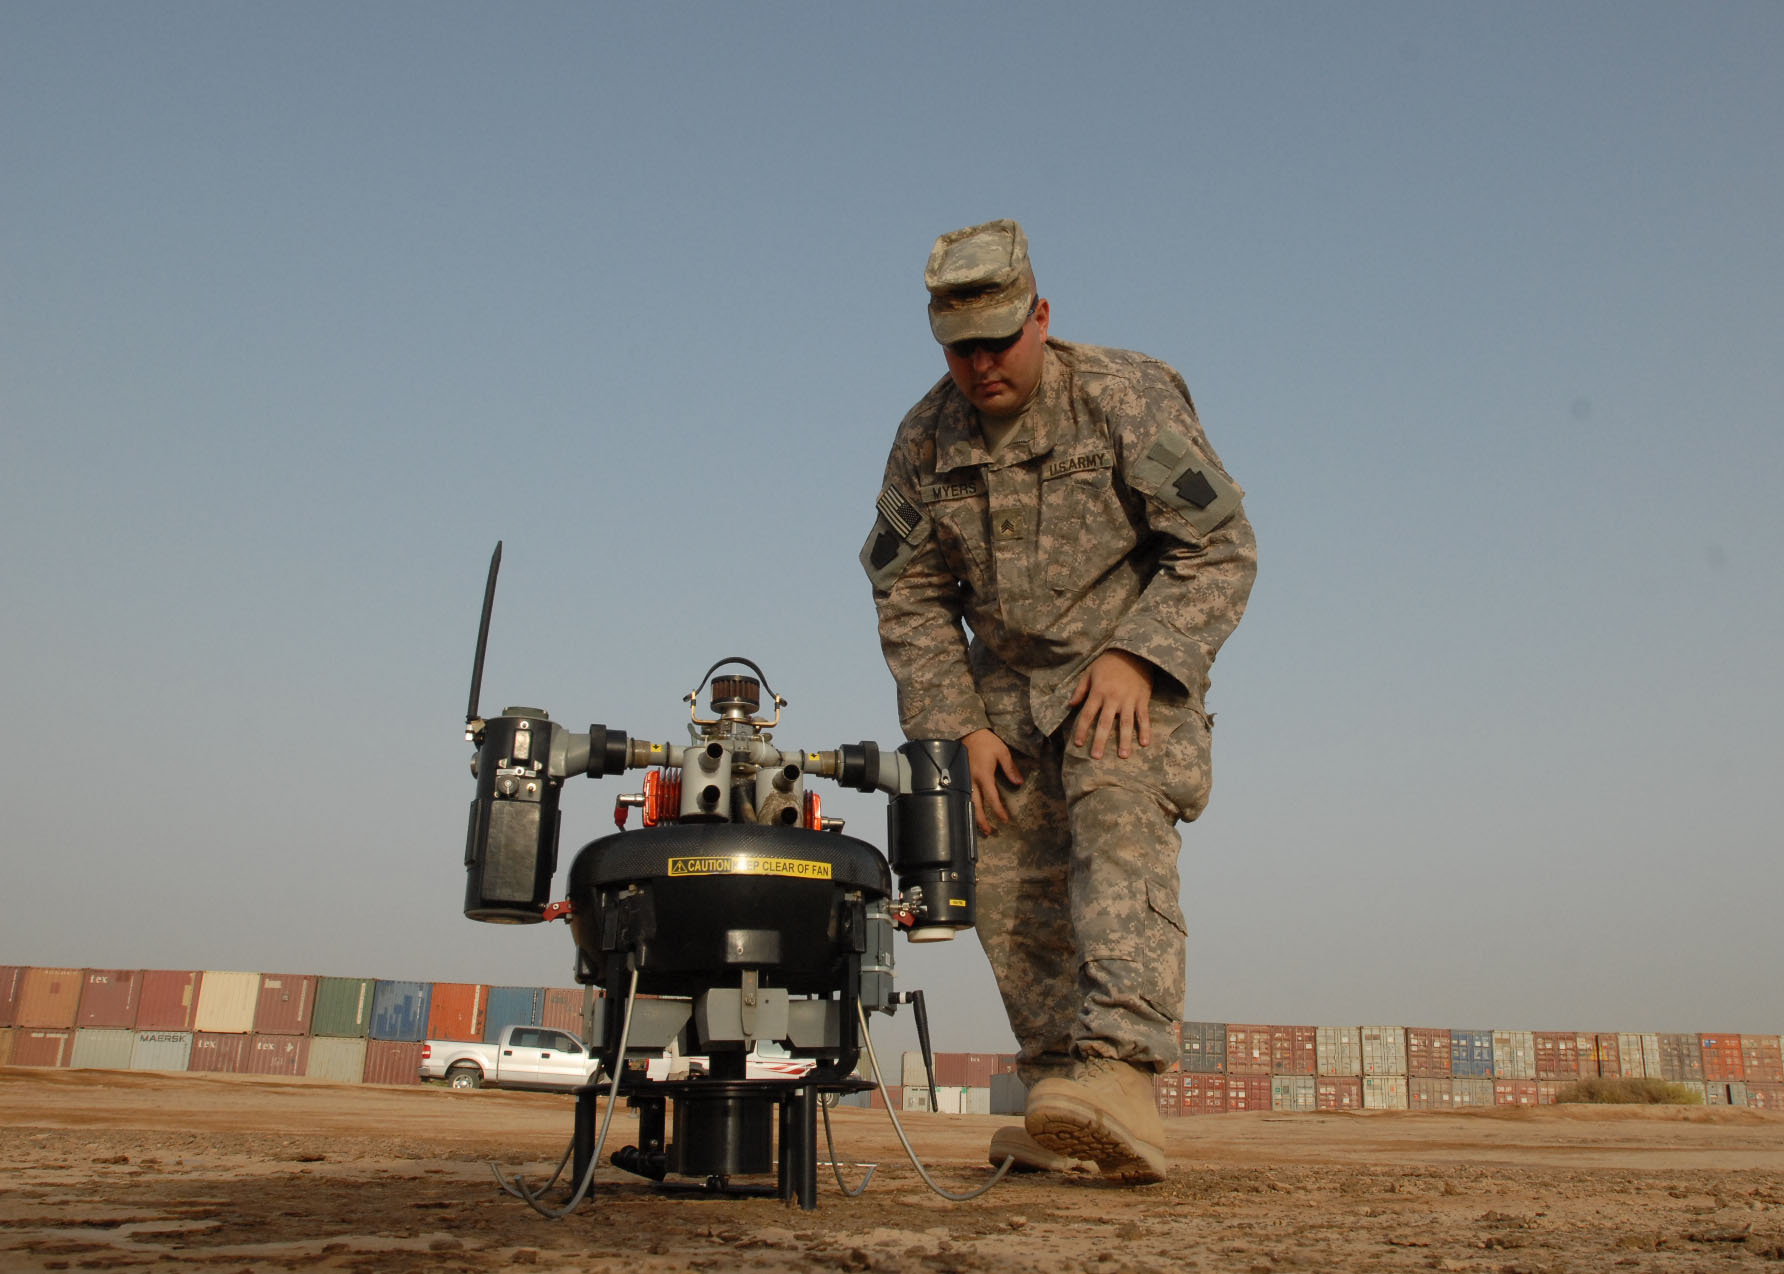
\includegraphics[width=4cm]{images/bitmap_image}
  \caption{Exemple d'image au format JPG.}
  \label{fig:une-autre-image}
\end{figure}

%%% Local Variables: 
%%% mode: latex
%%% TeX-master: "../roque-phdthesis"
%%% End: 

% \chapter{Un chapitre}
\label{sec:unchapitre}
\minitoc

Lorem ipsum dolor sit amet, consectetur adipiscing elit \cite{Bello1963}. Sed non risus. Suspendisse lectus tortor, dignissim sit amet, adipiscing nec, ultricies sed, dolor. Cras elementum ultrices diam. Maecenas ligula massa, varius a, semper congue, euismod non, mi. Proin porttitor, orci nec nonummy molestie, enim est eleifend mi, non fermentum diam nisl sit amet erat. Duis semper. Duis arcu massa, scelerisque vitae, consequat in, pretium a, enim. Pellentesque congue. Ut in risus volutpat libero pharetra tempor. Cras vestibulum bibendum augue. Praesent egestas leo in pede. Praesent blandit odio eu enim. Pellentesque sed dui ut augue blandit sodales. Vestibulum ante ipsum primis in faucibus orci luctus et ultrices posuere cubilia Curae; Aliquam nibh. Mauris ac mauris sed pede pellentesque fermentum. Maecenas adipiscing ante non diam sodales hendrerit. Ut velit mauris, egestas sed, gravida nec, ornare ut, mi. Aenean ut orci vel massa suscipit pulvinar. Nulla sollicitudin. Fusce varius, ligula non tempus aliquam, nunc turpis ullamcorper nibh, in tempus sapien eros vitae ligula. Pellentesque rhoncus nunc et augue. Integer id felis. Curabitur aliquet pellentesque diam. Integer quis metus vitae elit lobortis egestas. Lorem ipsum dolor sit amet, consectetuer adipiscing elit. Morbi vel erat non mauris convallis vehicula. Nulla et sapien. Integer tortor tellus, aliquam faucibus, convallis id, congue eu, quam. Mauris ullamcorper felis vitae erat. Proin feugiat, augue non elementum posuere, metus purus iaculis lectus, et tristique ligula justo vitae magna. Aliquam convallis sollicitudin purus. Praesent aliquam, enim at fermentum mollis, ligula massa adipiscing nisl, ac euismod nibh nisl eu lectus. Fusce vulputate sem at sapien. Vivamus leo. Aliquam euismod libero eu enim. Nulla nec felis sed leo placerat imperdiet. Aenean suscipit nulla in justo. Suspendisse cursus rutrum augue. Nulla tincidunt tincidunt mi. Curabitur iaculis, lorem vel rhoncus faucibus, felis magna fermentum augue, et ultricies lacus lorem varius purus. Curabitur eu amet.

\begin{figure}[htp!]
  \centering
  \setlength\figureheight{7cm}
  \setlength\figurewidth{9cm}
  % This file was created by matlab2tikz v0.2.2.
% Copyright (c) 2008--2012, Nico Schlömer <nico.schloemer@gmail.com>
% All rights reserved.
% 
% 
% 

% defining custom colors
\definecolor{mycolor1}{rgb}{0,0.75,0.75}

\begin{tikzpicture}

\begin{axis}[%
view={0}{90},
width=\figurewidth,
height=\figureheight,
scale only axis,
xmin=2, xmax=4.5,
xlabel={$\eta$},
xmajorgrids,
ymin=0.5, ymax=1,
ylabel={$d_{\text{min}}^2$},
ymajorgrids,
legend cell align=left,
legend style={align=left}]
\addplot [
color=black,
dashed,
mark=asterisk,
mark options={solid}
]
coordinates{
 (2,1)(2.1,1)(2.2,1)(2.3,1)(2.4,1)(2.5,1)(2.6,0.937749781479547)(2.7,0.890900393128398)(2.8,0.864988513955105)(2.9,0.827013168393703)(3,0.811347612650328)(3.1,0.792559278041243)(3.2,0.765840563467819)(3.3,0.749680961469385)(3.4,0.741947149227874)(3.5,0.740609493518419)(3.6,0.732128087463441)(3.7,0.717775843626632)(3.8,0.699687461812158)(3.9,0.685018622769455)(4,0.673439611642851)(4.1,0.664624248264608)(4.2,0.658255928882634)(4.3,0.641702335270489)(4.4,0.608326504614558)(4.5,0.580489221369454) 
};
\addlegendentry{$\alpha\text{ =  0\%}$};

\addplot [
color=black,
dashed,
mark=x,
mark options={solid}
]
coordinates{
 (2,1)(2.1,1)(2.2,1)(2.3,1)(2.4,0.958561324724996)(2.5,0.900812804739278)(2.6,0.859608621629443)(2.7,0.828484932127753)(2.8,0.812298837741994)(2.9,0.778916291864501)(3,0.758500630955482)(3.1,0.748375165853317)(3.2,0.745960208532468)(3.3,0.738441167434538)(3.4,0.715506361296671)(3.5,0.696927131434508)(3.6,0.682276848692725)(3.7,0.671128156410174)(3.8,0.663062783265717)(3.9,0.657680299791254)(4,0.621142740976429)(4.1,0.589786339121755)(4.2,0.564530571776849)(4.3,0.54483432747474)(4.4,0.53008799514765)(4.5,0.519641830384595) 
};
\addlegendentry{$\alpha\text{ = 10\%}$};

\addplot [
color=black,
dashed,
mark=triangle,
mark options={solid}
]
coordinates{
 (2,1)(2.1,1)(2.2,1)(2.3,0.966145915091813)(2.4,0.907589260275562)(2.5,0.862273165052718)(2.6,0.833762738286283)(2.7,0.797262289343802)(2.8,0.774689700869446)(2.9,0.763077871790574)(3,0.759584455148894)(3.1,0.735410358863577)(3.2,0.713220246811223)(3.3,0.695713299974315)(3.4,0.682371019886023)(3.5,0.672682085917092)(3.6,0.6661550402729)(3.7,0.644666127799479)(3.8,0.610083129739041)(3.9,0.582172698611821)(4,0.560333265725228)(4.1,0.543883933286703)(4.2,0.532098369213191)(4.3,0.524242326405)(4.4,0.519608701974017)(4.5,0.517545187250875) 
};
\addlegendentry{$\alpha\text{ = 20\%}$};

\addplot [
color=black,
dashed,
mark=triangle,
mark options={solid,,rotate=180}
]
coordinates{
 (2,1)(2.1,1)(2.2,0.995488894312993)(2.3,0.930050749246739)(2.4,0.882604857341179)(2.5,0.840148695151764)(2.6,0.807621264874927)(2.7,0.787889977099099)(2.8,0.777972678915356)(2.9,0.750463202108443)(3,0.726620292578349)(3.1,0.707917379352703)(3.2,0.693763185722015)(3.3,0.683575144048861)(3.4,0.676795290182409)(3.5,0.663350261880571)(3.6,0.627666127013326)(3.7,0.598755039468926)(3.8,0.575986310488554)(3.9,0.558651995817327)(4,0.546003746104731)(4.1,0.537291509323841)(4.2,0.531798375059385)(4.3,0.528867181690889)(4.4,0.527917002741411)(4.5,0.528450017604181) 
};
\addlegendentry{$\alpha\text{ = 30\%}$};

\addplot [
color=black,
dashed,
mark=o,
mark options={solid}
]
coordinates{
 (2,1)(2.1,1)(2.2,1)(2.3,1)(2.4,1)(2.5,0.995096871086856)(2.6,0.937749790013923)(2.7,0.890900391028178)(2.8,0.864988509535523)(2.9,0.827013167946275)(3,0.811347609462027)(3.1,0.79255927917077)(3.2,0.765840564829299)(3.3,0.749680963181722)(3.4,0.741947149533667)(3.5,0.740609492450166)(3.6,0.732128080624777)(3.7,0.71777584554089)(3.8,0.699687463368726)(3.9,0.681193180471954)(4,0.640212533267028)(4.1,0.617585040920557)(4.2,0.608519007405809)(4.3,0.608298095410932)(4.4,0.608326494076335)(4.5,0.580489212682311) 
};
\addlegendentry{Mazo};

\end{axis}
\end{tikzpicture}%
  \caption{Exemple de courbe TikZ.}
  \label{fig:courbe-tikz}
\end{figure}

\section{Description du modèle}
Lorem ipsum dolor sit amet, consectetur adipiscing elit. Sed non risus. Suspendisse lectus tortor, dignissim sit amet, adipiscing nec, ultricies sed, dolor. Cras elementum ultrices diam. Maecenas ligula massa, varius a, semper congue, euismod non, mi. Proin porttitor, orci nec nonummy molestie, enim est eleifend mi, non fermentum diam nisl sit amet erat. Duis semper. Duis arcu massa, scelerisque vitae, consequat in, pretium a, enim. Pellentesque congue. Ut in risus volutpat libero pharetra tempor. Cras vestibulum bibendum augue. Praesent egestas leo in pede. Praesent blandit odio eu enim. Pellentesque sed dui ut augue blandit sodales. Vestibulum ante ipsum primis in faucibus orci luctus et ultrices posuere cubilia Curae; Aliquam nibh. Mauris ac mauris sed pede pellentesque fermentum. Maecenas adipiscing ante non diam sodales hendrerit. Ut velit mauris, egestas sed, gravida nec, ornare ut, mi. Aenean ut orci vel massa suscipit pulvinar. Nulla sollicitudin. Fusce varius, ligula non tempus aliquam, nunc turpis ullamcorper nibh, in tempus sapien eros vitae ligula. Pellentesque rhoncus nunc et augue. Integer id felis. Curabitur aliquet pellentesque diam. Integer quis metus vitae elit lobortis egestas. Lorem ipsum dolor sit amet, consectetuer adipiscing elit. Morbi vel erat non mauris convallis vehicula. Nulla et sapien. Integer tortor tellus, aliquam faucibus, convallis id, congue eu, quam. Mauris ullamcorper felis vitae erat. Proin feugiat, augue non elementum posuere, metus purus iaculis lectus, et tristique ligula justo vitae magna. Aliquam convallis sollicitudin purus. Praesent aliquam, enim at fermentum mollis, ligula massa adipiscing nisl, ac euismod nibh nisl eu lectus. Fusce vulputate sem at sapien. Vivamus leo. Aliquam euismod libero eu enim. Nulla nec felis sed leo placerat imperdiet. Aenean suscipit nulla in justo. Suspendisse cursus rutrum augue. Nulla tincidunt tincidunt mi. Curabitur iaculis, lorem vel rhoncus faucibus, felis magna fermentum augue, et ultricies lacus lorem varius purus. Curabitur eu amet.

\section{Analyse aux limites}
Lorem ipsum dolor sit amet, consectetur adipiscing elit. Sed non risus. Suspendisse lectus tortor, dignissim sit amet, adipiscing nec, ultricies sed, dolor. Cras elementum ultrices diam. Maecenas ligula massa, varius a, semper congue, euismod non, mi. Proin porttitor, orci nec nonummy molestie, enim est eleifend mi, non fermentum diam nisl sit amet erat. Duis semper. Duis arcu massa, scelerisque vitae, consequat in, pretium a, enim. Pellentesque congue. Ut in risus volutpat libero pharetra tempor. Cras vestibulum bibendum augue. Praesent egestas leo in pede. Praesent blandit odio eu enim. Pellentesque sed dui ut augue blandit sodales. Vestibulum ante ipsum primis in faucibus orci luctus et ultrices posuere cubilia Curae; Aliquam nibh. Mauris ac mauris sed pede pellentesque fermentum. Maecenas adipiscing ante non diam sodales hendrerit. Ut velit mauris, egestas sed, gravida nec, ornare ut, mi. Aenean ut orci vel massa suscipit pulvinar. Nulla sollicitudin. Fusce varius, ligula non tempus aliquam, nunc turpis ullamcorper nibh, in tempus sapien eros vitae ligula. Pellentesque rhoncus nunc et augue. Integer id felis. Curabitur aliquet pellentesque diam. Integer quis metus vitae elit lobortis egestas. Lorem ipsum dolor sit amet, consectetuer adipiscing elit. Morbi vel erat non mauris convallis vehicula. Nulla et sapien. Integer tortor tellus, aliquam faucibus, convallis id, congue eu, quam. Mauris ullamcorper felis vitae erat. Proin feugiat, augue non elementum posuere, metus purus iaculis lectus, et tristique ligula justo vitae magna. Aliquam convallis sollicitudin purus. Praesent aliquam, enim at fermentum mollis, ligula massa adipiscing nisl, ac euismod nibh nisl eu lectus. Fusce vulputate sem at sapien. Vivamus leo. Aliquam euismod libero eu enim. Nulla nec felis sed leo placerat imperdiet. Aenean suscipit nulla in justo. Suspendisse cursus rutrum augue. Nulla tincidunt tincidunt mi. Curabitur iaculis, lorem vel rhoncus faucibus, felis magna fermentum augue, et ultricies lacus lorem varius purus. Curabitur eu amet.

\subsection{Calculer en cent leçons}
Lorem ipsum dolor sit amet, consectetuer adipiscing elit. Morbi vel erat non mauris convallis vehicula. Nulla et sapien. Integer tortor tellus, aliquam faucibus, convallis id, congue eu, quam. Mauris ullamcorper felis vitae erat. Proin feugiat, augue non elementum posuere, metus purus iaculis lectus, et tristique ligula justo vitae magna. Aliquam convallis sollicitudin purus. Praesent aliquam, enim at fermentum mollis, ligula massa adipiscing nisl, ac euismod nibh nisl eu lectus. Fusce vulputate sem at sapien. Vivamus leo. Aliquam euismod libero eu enim. Nulla nec felis sed leo placerat imperdiet. Aenean suscipit nulla in justo. Suspendisse cursus rutrum augue. Nulla tincidunt tincidunt mi. Curabitur iaculis, lorem vel rhoncus faucibus, felis magna fermentum augue, et ultricies lacus lorem varius purus. Curabitur eu amet.

\subsection{Le monde conique}
Lorem ipsum dolor sit amet, consectetuer adipiscing elit. Morbi vel erat non mauris convallis vehicula. Nulla et sapien. Integer tortor tellus, aliquam faucibus, convallis id, congue eu, quam. Mauris ullamcorper felis vitae erat. Proin feugiat, augue non elementum posuere, metus purus iaculis lectus, et tristique ligula justo vitae magna. Aliquam convallis sollicitudin purus. Praesent aliquam, enim at fermentum mollis, ligula massa adipiscing nisl, ac euismod nibh nisl eu lectus. Fusce vulputate sem at sapien. Vivamus leo. Aliquam euismod libero eu enim. Nulla nec felis sed leo placerat imperdiet. Aenean suscipit nulla in justo. Suspendisse cursus rutrum augue. Nulla tincidunt tincidunt mi. Curabitur iaculis, lorem vel rhoncus faucibus, felis magna fermentum augue, et ultricies lacus lorem varius purus. Curabitur eu amet.

\begin{align}
H_{m,n,p,q} &= \DPR{\rproto_{p,q}}{\OP{H} \tproto_{m,n}}\\
&= \iint\limits_{\SET{R}^2} S_{\OP{H}}(f,\tau) \DPR{\rproto_{p,q}}{\OP{U}_{f,\tau} \tproto_{m,n}} \ud f \ud \tau \\
&= \iint\limits_{\SET{R}^2} S_{\OP{H}}(f,\tau) \int\limits_{\R} \rproto_{p,q}^*(t) \OP{U}_{f,\tau} (\tproto_{m,n})(t) \ud t \ud f \ud \tau\\
&= \iint\limits_{\SET{R}^2} S_{\OP{H}}(f,\tau) \int\limits_{\R} \rproto^*(t-qT_0)e^{-j2 \pi pF_0t} \tproto(t-nT_0-\tau)e^{j2 \pi (mF_0(t-\tau) + ft)} \ud t \ud f \ud \tau\\
&= \iint\limits_{\SET{R}^2} S_{\OP{H}}(f,\tau) e^{-j2\pi m F_0 \tau} \int\limits_{\R} \rproto^*(t-qT_0) \tproto(t-nT_0-\tau)e^{j2 \pi ((m-p)F_0 + f)t} \ud t \ud f \ud \tau.
\end{align}

\section{Vérification par simulation numérique}
Lorem ipsum dolor sit amet, consectetur adipiscing elit. Sed non risus. Suspendisse lectus tortor, dignissim sit amet, adipiscing nec, ultricies sed, dolor. Cras elementum ultrices diam. Maecenas ligula massa, varius a, semper congue, euismod non, mi. Proin porttitor, orci nec nonummy molestie, enim est eleifend mi, non fermentum diam nisl sit amet erat. Duis semper. Duis arcu massa, scelerisque vitae, consequat in, pretium a, enim. Pellentesque congue. Ut in risus volutpat libero pharetra tempor. Cras vestibulum bibendum augue. Praesent egestas leo in pede. Praesent blandit odio eu enim. Pellentesque sed dui ut augue blandit sodales. Vestibulum ante ipsum primis in faucibus orci luctus et ultrices posuere cubilia Curae; Aliquam nibh. Mauris ac mauris sed pede pellentesque fermentum. Maecenas adipiscing ante non diam sodales hendrerit. Ut velit mauris, egestas sed, gravida nec, ornare ut, mi. Aenean ut orci vel massa suscipit pulvinar. Nulla sollicitudin. Fusce varius, ligula non tempus aliquam, nunc turpis ullamcorper nibh, in tempus sapien eros vitae ligula. Pellentesque rhoncus nunc et augue. Integer id felis. Curabitur aliquet pellentesque diam. Integer quis metus vitae elit lobortis egestas. Lorem ipsum dolor sit amet, consectetuer adipiscing elit. Morbi vel erat non mauris convallis vehicula. Nulla et sapien. Integer tortor tellus, aliquam faucibus, convallis id, congue eu, quam. Mauris ullamcorper felis vitae erat. Proin feugiat, augue non elementum posuere, metus purus iaculis lectus, et tristique ligula justo vitae magna. Aliquam convallis sollicitudin purus. Praesent aliquam, enim at fermentum mollis, ligula massa adipiscing nisl, ac euismod nibh nisl eu lectus. Fusce vulputate sem at sapien. Vivamus leo. Aliquam euismod libero eu enim. Nulla nec felis sed leo placerat imperdiet. Aenean suscipit nulla in justo. Suspendisse cursus rutrum augue. Nulla tincidunt tincidunt mi. Curabitur iaculis, lorem vel rhoncus faucibus, felis magna fermentum augue, et ultricies lacus lorem varius purus. Curabitur eu amet.

%%% Local Variables: 
%%% mode: latex
%%% TeX-master: "../roque-phdthesis"
%%% End: 

% \chapter*{Conclusion et perspectives}
\addstarredchapter{Conclusion}
\markboth{Conclusion}{Conclusion}
\label{sec:conclusion}

    Lorem ipsum dolor sit amet, consectetur adipiscing elit. Sed non risus. Suspendisse lectus tortor, dignissim sit amet, adipiscing nec, ultricies sed, dolor. Cras elementum ultrices diam. Maecenas ligula massa, varius a, semper congue, euismod non, mi. Proin porttitor, orci nec nonummy molestie, enim est eleifend mi, non fermentum diam nisl sit amet erat. Duis semper. Duis arcu massa, scelerisque vitae, consequat in, pretium a, enim. Pellentesque congue. Ut in risus volutpat libero pharetra tempor. Cras vestibulum bibendum augue. Praesent egestas leo in pede. Praesent blandit odio eu enim. Pellentesque sed dui ut augue blandit sodales. Vestibulum ante ipsum primis in faucibus orci luctus et ultrices posuere cubilia Curae; Aliquam nibh. Mauris ac mauris sed pede pellentesque fermentum. Maecenas adipiscing ante non diam sodales hendrerit. Ut velit mauris, egestas sed, gravida nec, ornare ut, mi. Aenean ut orci vel massa suscipit pulvinar. Nulla sollicitudin. Fusce varius, ligula non tempus aliquam, nunc turpis ullamcorper nibh, in tempus sapien eros vitae ligula. Pellentesque rhoncus nunc et augue. Integer id felis. Curabitur aliquet pellentesque diam. Integer quis metus vitae elit lobortis egestas. Lorem ipsum dolor sit amet, consectetuer adipiscing elit. Morbi vel erat non mauris convallis vehicula. Nulla et sapien. Integer tortor tellus, aliquam faucibus, convallis id, congue eu, quam. Mauris ullamcorper felis vitae erat. Proin feugiat, augue non elementum posuere, metus purus iaculis lectus, et tristique ligula justo vitae magna. Aliquam convallis sollicitudin purus. Praesent aliquam, enim at fermentum mollis, ligula massa adipiscing nisl, ac euismod nibh nisl eu lectus. Fusce vulputate sem at sapien. Vivamus leo. Aliquam euismod libero eu enim. Nulla nec felis sed leo placerat imperdiet. Aenean suscipit nulla in justo. Suspendisse cursus rutrum augue. Nulla tincidunt tincidunt mi. Curabitur iaculis, lorem vel rhoncus faucibus, felis magna fermentum augue, et ultricies lacus lorem varius purus. Curabitur eu amet.

    Lorem ipsum dolor sit amet, consectetur adipiscing elit. Sed non risus. Suspendisse lectus tortor, dignissim sit amet, adipiscing nec, ultricies sed, dolor. Cras elementum ultrices diam. Maecenas ligula massa, varius a, semper congue, euismod non, mi. Proin porttitor, orci nec nonummy molestie, enim est eleifend mi, non fermentum diam nisl sit amet erat. Duis semper. Duis arcu massa, scelerisque vitae, consequat in, pretium a, enim. Pellentesque congue. Ut in risus volutpat libero pharetra tempor. Cras vestibulum bibendum augue. Praesent egestas leo in pede. Praesent blandit odio eu enim. Pellentesque sed dui ut augue blandit sodales. Vestibulum ante ipsum primis in faucibus orci luctus et ultrices posuere cubilia Curae; Aliquam nibh. Mauris ac mauris sed pede pellentesque fermentum. Maecenas adipiscing ante non diam sodales hendrerit. Ut velit mauris, egestas sed, gravida nec, ornare ut, mi. Aenean ut orci vel massa suscipit pulvinar. Nulla sollicitudin. Fusce varius, ligula non tempus aliquam, nunc turpis ullamcorper nibh, in tempus sapien eros vitae ligula. Pellentesque rhoncus nunc et augue. Integer id felis. Curabitur aliquet pellentesque diam. Integer quis metus vitae elit lobortis egestas. Lorem ipsum dolor sit amet, consectetuer adipiscing elit. Morbi vel erat non mauris convallis vehicula. Nulla et sapien. Integer tortor tellus, aliquam faucibus, convallis id, congue eu, quam. Mauris ullamcorper felis vitae erat. Proin feugiat, augue non elementum posuere, metus purus iaculis lectus, et tristique ligula justo vitae magna. Aliquam convallis sollicitudin purus. Praesent aliquam, enim at fermentum mollis, ligula massa adipiscing nisl, ac euismod nibh nisl eu lectus. Fusce vulputate sem at sapien. Vivamus leo. Aliquam euismod libero eu enim. Nulla nec felis sed leo placerat imperdiet. Aenean suscipit nulla in justo. Suspendisse cursus rutrum augue. Nulla tincidunt tincidunt mi. Curabitur iaculis, lorem vel rhoncus faucibus, felis magna fermentum augue, et ultricies lacus lorem varius purus. Curabitur eu amet.

    Lorem ipsum dolor sit amet, consectetur adipiscing elit. Sed non risus. Suspendisse lectus tortor, dignissim sit amet, adipiscing nec, ultricies sed, dolor. Cras elementum ultrices diam. Maecenas ligula massa, varius a, semper congue, euismod non, mi. Proin porttitor, orci nec nonummy molestie, enim est eleifend mi, non fermentum diam nisl sit amet erat. Duis semper. Duis arcu massa, scelerisque vitae, consequat in, pretium a, enim. Pellentesque congue. Ut in risus volutpat libero pharetra tempor. Cras vestibulum bibendum augue. Praesent egestas leo in pede. Praesent blandit odio eu enim. Pellentesque sed dui ut augue blandit sodales. Vestibulum ante ipsum primis in faucibus orci luctus et ultrices posuere cubilia Curae; Aliquam nibh. Mauris ac mauris sed pede pellentesque fermentum. Maecenas adipiscing ante non diam sodales hendrerit. Ut velit mauris, egestas sed, gravida nec, ornare ut, mi. Aenean ut orci vel massa suscipit pulvinar. Nulla sollicitudin. Fusce varius, ligula non tempus aliquam, nunc turpis ullamcorper nibh, in tempus sapien eros vitae ligula. Pellentesque rhoncus nunc et augue. Integer id felis. Curabitur aliquet pellentesque diam. Integer quis metus vitae elit lobortis egestas. Lorem ipsum dolor sit amet, consectetuer adipiscing elit. Morbi vel erat non mauris convallis vehicula. Nulla et sapien. Integer tortor tellus, aliquam faucibus, convallis id, congue eu, quam. Mauris ullamcorper felis vitae erat. Proin feugiat, augue non elementum posuere, metus purus iaculis lectus, et tristique ligula justo vitae magna. Aliquam convallis sollicitudin purus. Praesent aliquam, enim at fermentum mollis, ligula massa adipiscing nisl, ac euismod nibh nisl eu lectus. Fusce vulputate sem at sapien. Vivamus leo. Aliquam euismod libero eu enim. Nulla nec felis sed leo placerat imperdiet. Aenean suscipit nulla in justo. Suspendisse cursus rutrum augue. Nulla tincidunt tincidunt mi. Curabitur iaculis, lorem vel rhoncus faucibus, felis magna fermentum augue, et ultricies lacus lorem varius purus. Curabitur eu amet.

%%% Local Variables: 
%%% mode: latex
%%% TeX-master: "../roque-phdthesis"
%%% End: 


\begin{document}
% \shorthandoff{:} % Commande pour enlever l'espace avant les deux points 

% Include the title pages
% (the first is made mandatory by UDG and the second is more traditional)
%%%%%%%%%%%%%%%%%%%%%%%%%%%
%%% Official title page from UDG  %%%
%%%%%%%%%%%%%%%%%%%%%%%%%%%
\begingroup
\fontsize{13pt}{13pt}\selectfont

\AddToShipoutPicture*{\BackgroundPic}
\def\leftshift{0.82\textwidth}
\def\espvert{0.25cm}
\setlength{\parskip}{0pt}
\begin{titlepage}
\begin{adjustwidth}{}{-3em}
\begin{flushleft}

~~

\vfill

\begin{flushright}
\begin{minipage}{\leftshift}
\begin{flushleft}
\textsc{\Large \bf THÈSE}\\[\espvert]
{pour obtenir le grade de}\\[\espvert]
\textsc{\Large \bf DOCTEUR DE L'UNIVERSITÉ DE GRENOBLE}\\[\espvert]
{Spécialité : \textbf{Informatique et Mathématiques appliquées}}\\[\espvert]
{Arrêté ministériel : 7 août 2006}
\end{flushleft}
\end{minipage}
\end{flushright}~~\\[0.75cm]

\vfill

\begin{flushright}
\begin{minipage}{\leftshift}
\begin{flushleft}
{Présentée par}\\
{\Large \textbf{Cao Tri DO}}
\end{flushleft}
\end{minipage}
\end{flushright}~~\\[0.75cm]

\vfill

\begin{flushright}
\begin{minipage}{\leftshift}
\begin{flushleft}
{
\begin{tabular}{lll}
	Thèse dirigée par 	& \textbf{Ahlame DOUZAL-CHOUAKRIA},	& \\
	codirigée par 		& \textbf{Michèle ROMBAUT} 			& et \\
	co-encadré par 		& \textbf{Sylvain MARI\'{E}} 		&
\end{tabular}	
}
\end{flushleft}
\end{minipage}
\end{flushright}

\vfill

\begin{flushright}
\begin{minipage}{\leftshift}
\begin{flushleft}
{préparée au sein du \\\textbf{Laboratoire d'Informatique de Grenoble (LIG)}\\
dans \textbf{l'école doctorale Mathématiques, Sciences et Technologies de l'Information, Informatique (MSTII)}}
\end{flushleft}
\end{minipage}
%\end{flushright}~~\\[1cm]
\end{flushright}~~\\[0.5cm]

\vfill

% Titre
\begin{flushright}
\begin{minipage}{\leftshift}
\begin{flushleft}
{ \Huge \bfseries Metric Learning for Time Series Analysis}
\end{flushleft}
\end{minipage}
%\end{flushright}~~\\[1cm]
\end{flushright}~~\\[0.6cm]
\vfill

% Jury
\begin{flushright}
\begin{minipage}{\leftshift}
\begin{flushleft}
{Thèse soutenue publiquement le \textbf{date de soutenance},\\ devant le jury composé de:}\\[\espvert]
% {\textbf{\president}}\\
% {\labopresident, Président}\\
{\textbf{Patrick GALLINARI}}\\
{Laboratoire LIP6, Examinateur }\\ % Président du jury
{\textbf{Stéphane CANU}}\\
{Laboratoire LITIS, Rapporteur}\\
{\textbf{Marc SEBBAN}}\\
{Laboratoire LAHC, Rapporteur}\\
{\textbf{Gustavo CAMPS-VALLS}}\\
{Laboratoire IPL, Examinateur}\\
% {\textbf{Benoît JACQUEMIN}}\\
% {Schneider Electric, Examinateur}\\
{\textbf{Ahlame DOUZAL-CHOUAKRIA}}\\
{Laboratoire LIG, Directeur de thèse}\\
{\textbf{Michèle ROMBAUT}}\\
{Laboratoire GIPSA-Lab, Co-Directeur de thèse}\\
{\textbf{Sylvain MARI\'{E}}}\\
{Schneider Electric, Encadrant}\\

\end{flushleft}
\end{minipage}
\end{flushright}
\vfill
\end{flushleft}
\end{adjustwidth}
\end{titlepage}
\setlength{\parskip}{10pt}
\endgroup

\cleardoublepage

%%%%%%%%%%%%%%%%%%%%%
%%% Traditional title page %%%
%%%%%%%%%%%%%%%%%%%%%
\cleardoublepage
\begin{titlepage}
\begin{center}
\noindent {\large \textbf{UNIVERSITÉ DE GRENOBLE}} \\
\vspace*{0.3cm}
\noindent {\LARGE \textbf{ÉCOLE DOCTORALE MSTII}} \\
\noindent \textbf{Description de complète de l'école doctorale} \\
\vspace*{0.5cm}
\noindent \Huge \textbf{T H È S E} \\
\vspace*{0.3cm}
\noindent \large {pour obtenir le titre de} \\
\vspace*{0.3cm}
\noindent \LARGE \textbf{docteur en sciences} \\
\vspace*{0.3cm}
\noindent \Large de l'Université de Grenoble-Alpes\\
\noindent \Large \textbf{Mention : \textsc{Informatique et Mathématiques appliquées}}\\
\vspace*{0.4cm}
\noindent \large {Présentée et soutenue par\\}
\noindent \LARGE Cao Tri DO \\
\vspace*{0.8cm}
\noindent {\Large \textbf{Metric Learning for Time Series Analysis}} \\
\vspace*{0.8cm}
\noindent \Large Thèse dirigée par Ahlame DOUZAL-CHOUAKRIA\\
\vspace*{0.2cm}
\noindent \Large préparée au Laboratoire d'Informatique de Grenoble (LIG) \\
\vspace*{0.2cm}
\noindent \large soutenue le date de soutenance \\
\vspace*{0.5cm}
\end{center}
\noindent \large \textbf{Jury :} \\
\begin{center}
\noindent \large 
\begin{tabular}{llcl}
      \textit{Rapporteurs :}	& Stéphane CANU		& - & Laboratoire LITIS\\
                				& Marc SEBBAN		& - & Laboratoire LAHC\\
      \textit{Directeur :}	    & Ahlame DOUZAL-CHOUAKRIA & - & Laboratoire LIG\\
      \textit{Co-Directeur :}	& Michèle ROMBAUT	& - & Laboratoire GIPSA-Lab\\
      \textit{Encadrant :}	    & Sylvain MARI\'{E}	& - & Schneider Electric\\
      \textit{Examinateur :}	& Patrick GALLINARI	& - & Laboratoire LIP6\\
      \textit{Examinateur :}    & Gustavo CAMPS-VALLS & - & Laboratoire IPL\\
\end{tabular}
\end{center}
\end{titlepage}
\sloppy

\titlepage

%%% Local Variables: 
%%% mode: latex
%%% TeX-master: "../roque-phdthesis"
%%% End: 


% Build a per-chapter table of content
\dominitoc

% Use roman page numbering for non-significant pages
\pagenumbering{roman}
\frontmatter

% Include the acknowledgements page
\cleardoublepage
\listoftodos


\chapter*{Acknowledgements}
%\noindent I would like to thanks:
%\begin{itemize}
%	\item my directors
%	\item my GIPSA collegues
%	\item my AMA collegues
%	\item my Schneider collegues
%	\item my parents
%\end{itemize}


%%% Local Variables: 
%%% mode: latex
%%% TeX-master: "../roque-phdthesis"
%%% End: 

C'est au moment des remerciements que vient la plus grand peur, celle d'oublier quelqu'un ... Pour parer à cette éventualité, je commencerai par remercier toutes les personnes qui m'ont aidé et soutenu pendant ces années.

Je remercie tout d'abord mes directeurs de thèse, Ahlame, Michèle et Sylvain, qui m'ont encadré pendant ces 3 années de thèse, et même avant, dès mon stage de Master 2, pour m'avoir donné les connaissances en Machine Learning, la patience et la rigueur en recherche. Malgré les moments difficiles que nous avons pu rencontrer lors de la thèse, ils ont toujours su m'aider à tenir le bon cap pour arriver aujourd'hui à ce travail d'une excellente qualité. Un grand merci à Ahlame pour m'avoir suivi sur le plan scientifique en me guidant sur la rigueur de recherche et d'écriture; à Sylvain, pour nous avoir partagé ses idées bouillonnantes et sa motivation en tant qu'ingénieur et chercheur; et enfin à Michèle pour son encadrement, son écoute et ses conseils généraux qu'elle a pu me donner pendant ces 3 années.

Je remercie ensuite les membres du jury, Stéphane Canu et Marc Sebban. Je mesure la chance que j'ai de vous avoir comme rapporteurs. Je remercie à vous et aux autres membres, Patrick Gallinari et Gustavo Camps-Valls, pour vos remarques sur le manuscrit, les questions posées et l'intérêt que vous avez porté à ces travaux.

Je remercie également mes collègues de Gipsa, Laetitia, Lyuba, Stefen, Thibault, Jaume, Victor et leurs petit(e)s ami(e)s, Alexandre et Lilia, pour ces années passées avec vous dans le bureau 1131 où on a pu partager des bons moments de thèse et aussi des moments de doute. Votre soutien moral, nos discussions scientifiques et nos sortis Gipsa ont été pour moi un élément que je n'oublierai jamais de cette expérience !

Je n'oublie pas mes collègues de AMA qui cette fois sont nombreux (Saeid, Georgios, Adrian, Bikash, Simon, Irina, Jidong, Fabien et tous les autres) qui ont su m'accueillir alors que je n'ai pas pu être là très souvent. Votre gentillesse et les moments passés lors des séminaires au vert de l'équipe ont été des moments de partage que je garderai en souvenir.

De même, je remercie chacun des permanents des 2 équipes (très nombreux que je ne peux tous citer): Gipsa et AMA pour leur accueil, leurs conseils et leurs retours qu'ils ont pu m'apporter sur ma thèse pendant ces 3 années et qui m'ont permis de construire mon projet de thèse.

A tous mes collègues de Schneider, permanents (Daniel, Franck, Jean Louis, Vincent, Véronique, Henri, Olivier, Rodolph, Alfredo, Laurent, Patrick, Yvon, France, Yassine, Bartosz), doctorants (Peter, Chloé, Benoit, Thibaud), presta (Yvon, Pierre, Nelly, Romain, Sophie, Gregory), stagiaires (Léa, Blaise) et alternants (Matthieu, Thomas, Amadou, Omar) qui ont su me faire découvrir l'environnement Schneider pendant ces 4 ans au sein de l'équipe A4S. Un remerciement tout particulier à Didier, Claude et François pour nous avoir soutenu dans ce projet de thèse et pour nous avoir toujours fait des retours pertinents sur le plan scientifique de la thèse. Et enfin, je n'oublierai jamais le A4S Band avec Matthieu et Peter où on a pu apporter la petite touche musicale de variété internationale dans Schneider. Il y a bien sûr tous les autres collègues de Schneider des autres équipes que je tenais à remercier pour ces années, notamment Benoît, qui a été à l'origine avec Patrice de ce projet.

Je remercie tous les amis qui sont venus de loin (Lyon, Avignon, Marseille, Montpellier, Pau, Paris et de la Suisse) pour le jour de la soutenance. Cela m'a beaucoup touché que vous ayez pu faire le déplacement. Un remerciement également à mes amis de Grenoble pour avoir pu partager ce moment avec vous, et un remerciement tout particulier à ma petite élève Candice et ses parents, Pascale et Claude, qui sont venus voir leur professeur de guitare présenté pour une fois autre chose que de la musique.

De manière générale, je remercie tous mes amis (français, québécois, allemands, vietnamiens, chinois, japonais, péruviens, espagnols), mes colocataires (Lauren, Laurence et Quentin) et ma famille qui ont contribué tout au long de ma thèse à veiller à son bon déroulement et à mes parents en particulier pour leur soutien moral et leur aide qui m'ont donné dans ces derniers jours avec le buffet de thèse et le déménagement.

Enfin, je terminerai ces remerciements à ma chère Louise, celle sans qui rien n'aurait pu être possible et qui m'a soutenu très largement pendant ces 3 ans !

Un grand merci à tous !

% Build the general table of contents
\setcounter{tocdepth}{1}
\tableofcontents

% Build the list of figures
\listoffigures

% Build the list of tables
\listoftables

% Include the acronym list
\cleardoublepage
\chapter*{Table of Acronyms}
%\chapter*{Table des sigles et acronymes}
\addstarredchapter{Table des sigles et acronymes}
\markboth{Table des sigles et acronymes}{Table des sigles et acronymes}

% Remember to use italic fonts for foreign words
\begin{acronym}[CP-OFDMX] % Specify the longest acronym in order to set the first column width
\acro{LIG}{\emph{Laboratoire d'Informatique de Grenoble}}
\acro{AMA}{\emph{Apprentissage, Méthode et Algorithme}}
\acro{GIPSA-Lab}{\emph{Grenoble Images Parole Signal Automatique Laboratoire}}
\acro{AGPiG}{\emph{Architecture, Géométrie, Perception, Images, Gestes}}
\acro{A4S}{\emph{Analytic for Solutions}}
\acro{$k$-NN}{\emph{$k$-nearest neighbors}}
\acro{SVM}{\emph{Support Vector Machines}}
\acro{SVR}{\emph{Support Vector Regression}}
\acro{$d_E$}{\emph{Euclidean distance}}
\acro{$corr$}{\emph{Pearson correlation}}
\acro{$cort$}{\emph{Temporal correlation}}
\acro{dtw}{\emph{Dynamic Time Warping}}
\acro{IoT}{\emph{Internet of Things}}
\acro{Acc}{\emph{Classification accuracy}}
\acro{Err}{\emph{Classification error rate}}
\acro{MAE}{\emph{Mean Absolute Error}}
\acro{RMSE}{\emph{Root Mean Square Error}}
\acro{FAQ}{Frequently Asked Questions / Foire Aux Questions}
\end{acronym}

% To cite an acronym in the text : \ac{ASK}
% To cite an acronym in the text without footnote : \acs{ASK}

%%% Local Variables: 
%%% mode: latex
%%% TeX-master: "../roque-phdthesis"
%%% End: 


%%%%%%%%%%%%%%%%%%%%%%%%%%
%%% Chapters are included here %%%
%%%%%%%%%%%%%%%%%%%%%%%%%%

% Use arabic page numbering for significant pages
\mainmatter
\pagestyle{fancy}

% Include the chapters
\chapter*{Introduction}
\addstarredchapter{Introduction}
\markboth{Introduction}{Introduction}
\label{chap:introduction}
%\minitoc

\section*{Motivation}
%\begin{itemize}
%	\item Mettre le contexte de la thèse : thèse CIFRE avec Schneider et 2 laboratoires de Grenoble.
%	\item Qu’est-ce qu’une série temporelle ? (réponse d’un système dynamique complexe (= pas de modèle du système)
%	\item Motiver l’intérêt des séries temporelles dans les applications aujourd’hui:  données de plus en plus présentes dans de nombreux domaines divers et variés
%	\item Les séries temporelles sont impliquées dans des problèmes de classification, régression et clustering
%	\item Pourquoi sont-elles challenging ? (délais, dynamique)
%	\item Intérêt dans le cadre des activités de Schneider Electric
%\end{itemize}
The work of this PhD is in the context of a CIFRE\footnote[1]{Conventions Industrielles de Formation par la REcherche} thesis with Schneider Electric and two public research laboratories, LIG\footnote[2]{Laboratoire d'Informatique de Grenoble} and GIPSA-lab\footnote[3]{Grenoble Images Parole Signal Automatique}. Within Schneider Electric, the PhD took place in the Analytics for Solutions (A4S) team, part of the Technology and Strategy entity. Among the wide rage of activities of the A4S team, in the context of system modeling (\textit{e.g.}, buildings, sensor networks, Internet of Things), two topics are at least studied: modeling by physical models (white/grey-box) and modeling by machine learning algorithms (black-box). With the increase of the amount of data and sensors that collect data, modeling accurately systems through \textit{a priori} equations (white/grey-box) for some prediction tasks has become more and more difficult. Within the vast amount of applications in Schneider Electric, some applications involve in particular temporal data, \textit{e.g.}, forecasting the energy consumption in a building, virtual sensors for industrial processes, fault detection and prediction for assets maintenance. More generally, Schneider Electric, like many other companies in various application domains (medicine, marketing, meteorology, etc.) has taken a growing interest these last decades in machine learning problems (classification, regression, clustering) that involve time series of one or several dimensions, of different samplings, etc. A time series can be seen in signal processing and in control theory as the response of a dynamic system. Contrary to static data, time series are more challenging in the sense that the temporal aspect (\textit{i.e.}, order of appearance of the observations) is an additional key information. \\

\section*{Problem statement and contributions}
In this work, we focus on classification problems of monovariate time series (data of 1 dimension) with a fixed sampling rate and of same fixed lengths. Among the wide variety of algorithms that exist in machine learning, some approaches (\textit{e.g.}, $k$-Nearest Neighbors ($k$-NN)) classify samples using a concept of neighborhood based on the comparison between samples. In general, the concepts of 'near' and 'far' between samples is expressed through a distance measure. Time series can be compared based not only on their amplitudes like static data but also on other characteristics, called modalities, such as their dynamics or frequency components. Many metrics for time series have been proposed in the literature such as the Euclidean distance \cite{Ding2008}, the temporal correlation \cite{Frambourg2013a}, the Fourier-based distance \cite{Sahidullah2012a}. A detailed review of the major metrics is proposed in \cite{Montero2014}. In general, existing metrics involve one modality (characteristic) at the global scale (\textit{i.e.}, involving systematically all the time series observations). We believe also that the multi-scale aspect of time series (\textit{i.e.}, involving a temporal part of the observations), not present in static data, could enrich the definition of the existing metrics. 

% \section*{Problem statement (with words)}
%\begin{itemize}
%	\item Dans de nombreux algorithmes de classification ou de régression (kNN, SVM), la comparaison des individus (séries temporelles) reposent sur une notion de distance entre individus (séries temporelles).
%	\item Contrairement aux données statiques, les données temporelles peuvent être comparés sur la base de plusieurs modalités (valeurs, forme, distance entre spectre, etc.) et à différentes échelles. La « métrique idéale », càd, celle qui permettra de résoudre au mieux le problème de classification/régression peut donc impliquer plusieurs modalités.
%	\item Objectif de notre travail : Apprendre une métrique adéquate tenant compte de plusieurs modalités et de plusieurs échelles en vue d’une classification/régression kNN
%\end{itemize}
In this work, our objective is to learn a combined multi-modal and multi-scale time series metric for a robust $k$-NN classifier. The main contributions of the PhD are:
\begin{itemize}
	\item[-] The definition of a new space representation: the pairwise dissimilarity space where each pair of time series is embedded as a vector described by basic temporal metrics.
	\item[-] The definition of basic temporal metrics that involve one modality at one specific scale.
	\item[-] The learning of a multi-modal and multi-scale temporal metric for a large margin $k$-NN classifier of univariate time series. 
	\item[-] The definition of the general problem of learning a combined metric as a metric learning problem using the dissimilarity representation. 
	\item[-] The proposition of a framework based on Support Vector Machine (\textsc{svm}) and a linear and non-linear solution to define the combined metric that satisfies at least the properties of a dissimilarity measure.
	\item[-] The comparison of the proposed approach with standard metrics on a large number of public datasets.
	\item[-] The analysis of the proposed approach to extract the discriminative features that are involved in the definition of the learned combined metric. 
\end{itemize}


%\section*{PhD contributions}
%\begin{itemize}
%	\item Définition d’un nouvel espace de représentation: la représentation par paires
%	\item Apprentissage d’une métrique multimodale et multi-échelle en vue d’une classification kNN à vaste marge de séries temporelles monovariées.
%	\item Définition du problème d’apprentissage de métrique combinée (Metric Learning) dans l’espace des paires sous la forme d'un problème général d'optimisation.
%	\item Comparaison de la méthode proposée avec des métriques classiques sur un vaste jeu de données (30 bases) de la littérature dans le cadre de la classification univariée de séries temporelles
%	\item Donner une solution interprétable.
%\end{itemize}

\section*{Organization of the manuscript}
\indent The first part makes a review of existing methods in machine learning and metrics for time series. The first chapter presents classical approaches in machine learning. We recall the general principle and framework in supervised learning and focus on two machine learning algorithms: the $k$-Nearest Neighbors ($k$-NN) and the Support Vector Machine (\textsc{svm}). In the second chapter, we review some basic terminology for time series and recall at least three types of metrics proposed for time series: amplitude-, behavior- and frequential-based. \\
\noindent The second part of the manuscript proposes a Multi-modal and Multi-scale Temporal Metric Learning (\textsc{m$^2$tml}) approach for a robust $k$-NN classifier of time series. In the third chapter, we first review the concept of metric learning for static data and focus on a framework of metric learning for nearest neighbors classification proposed by Weinberger \& Saul \cite{Weinberger2009}. We then present a new space representation, the pairwise dissimilarity space based on a multi-modal and multi-scale time series description and their corresponding basic metrics. Then, we formalize the general \textsc{m$^2$tml} optimization problem using the pairwise dissimilarity space representation. From the general formalization, we propose at least three different formalizations. The first and second propositions involve different regularizers, allowing to learn an \textit{a priori} linear or non-linear form of the combined metric. The third proposition presents a framework based on \textsc{svm} and a solution to build the combined metric, in the linear and non-linear context, satisfying at least the properties of a dissimilarity measure. Finally, Chapter 4 presents the experiments conducted on a wide range of 30 public and challenging datasets, and discusses the results obtained.

% Présenter les différents chapitres

%Note pour Ahlame, Michèle et Sylvain: Pour ajouter des commentaires dans le fichier .TEX, merci de les ajouter sous cette forme:
%\begin{itemize}
%	\item dans le texte : \myincomment[CTD]{Initial in [CAO] then your comment in the bracket}
%	\item dans la marge : \mycomment[CTD]{Initial in [CAO] then your comment in the bracket}
%\end{itemize}
%If you think that they are missing figures, you can add them with a description with this command line :
%\missingfigure{Testing a long text string}

\newpage
\section*{Industrial motivations: analytics context within Schneider Electric}
\begin{itemize}
	\item Idée : raccrocher les problématiques de Schneider aux problématiques scientifiques
	\item Part 1 : Problème autour de la segmentation des séries temporelles : qu'est ce qu'une série temporelle en industrie?
	\item Part 2 : Les types de problèmes en Machine Learning en lien avec le voca de l'industrie
	\item L'évolution des technologies dans la collecte des données ces dernières décennies a posé de nouveaux intérêts et enjeux : comment tirer parti au mieux des données massives provenant de plusieurs sources pour aider les industries à être plus efficaces dans leurs activités de développement de solutions (services, etc.) qui leur permettent d'être plus efficaces (construction de modèles, coût, temps, précision, etc.).
	\item Le terme à la mode "Analytics" est souvent utilisés pour désigner ces efforts mais les frontières de sa définition reste assez flous (donner des exemples?). Ceci peut générer des incompréhensions entre les domaines (industries, recherche, etc.).
	\item Dans le même temps, l'évolution des technologies a permis de donner une nouvelle dimension dans l'étude des données : la temporalité. Pour désigner des données qui évoluent dans le temps, on utilise souvent le terme de séries temporelles mais la définition mathématiques et industrielles (y compris pour différents domaines ou applications) peuvent connaître quelques différences.
	\item L'idée ici est de 1) Poser une définition des Analytics; 2) Formaliser le terme de séries temporelles; 3) Donner les liens de voca entre l'académique et l'industrie. 
	\item La définition d'un terme comme "Analytics" doit répondre à 2 questions : qu'est ce que c'est, et qu'est ce que ça fait (what it is, what it does): "Analytics is the process of developing actionable insights through problem definition and the application of statistical models and analysis against existing and/or simulated future data."
	\item Expliquer ce que veut dire "actionable insights"
	\item Prendre la définition des Analytics de l'équipe
	\item Définir le terme séries temporelles (peut être vues comme une extension des données statiques en tenant compte de la séquentialité des données) En industrie, une série temporelle peut représenter différents objets ou entités en fonction du choix de segmentation/découpage qui leur ai fait (\textit{i.e.}, choisir le début et la fin de la série temporelle). Pas très claire et intuitif pour moi
	\item Problème de la segmentation des séries temporelles : liés à l'application.
	\begin{itemize}
		\item si le but est de reconnaître un pattern dans une longue série temporelle
		\item si le but est de prédire une valeur à partir d'une fenêtre temporelle
		\item etc.
	\end{itemize}
	\item Les problèmes généraux des Analytics pour les séries temporelles 
	\begin{itemize}
		\item Supervisé / semi-supervisé
		\begin{itemize}
			\item Classification : assign a time series to a pre-defined class
			\begin{itemize}
				\item One-class = outlier detection. (Application: Fault dectection)
				\item Two-class (particular case of multi-class problems)
				\item Multi-class = classification. (Application: diagnosis, situation assement, pattern matching)
			\end{itemize}
			\item Régression : predict a (real) number = scoring, prediction, regression (Application: Virtual Sensor, Forecasting)
		\end{itemize}
		\item Clustering : separate a dataset into distinct non-given groups/class = profiling, segmentation.
	\end{itemize}
\end{itemize}

In the last decades, the evolution in data collection technologies has raised new interests and challenges: how to get the best from the massive growing amount data coming from several sources to help industries in their activities to develop solutions (services, etc.) that can make them more effective (\textit{e.g.}, cost, time or accuracy in system modeling\footnote{the word modeling is used in its broad sense, encompassing prediction, fault detection, profiling, etc.}). The word "Analytics" is often used to describe the efforts that goes in that sense. However, like many other buzz-words, the frontier of its definition may be vague and it can lead to misunterstading or the appearance of several words for a same concept, either between various actors (industrial, academics, etc.) or worst, between collaborators working in the same company but in different teams. \\
Meanwhile, the ability of collecting easily data has allowed to take into account of an other characteristics in the data: the temporality. To designate data that evolves over the time, the word "time series" is often used but the



\part{Work positionning}

The first part of the manuscript aims to position the work context. Our objective is the comparison and the classification or regression of time series. The first chapter considers time series as static vector data and presents classic machine learning algorithms used to classify them. We note that most of these methods relies on the comparison of objects (time series in our case) through a distance measure. In the second chapter, to cope with the characteristics of time series (amplitude, behavior, frequential spectrum, etc.), we recall some basic metrics used to compare time series. We show that time series may be compared by several modalities and at different granularities. We finally cast that learning an adequate distance based on several modalities and several granularities is a key challenge nowadays to well classify time series using classic machine learning algorithms.


\chapter{Related work}
\label{chap:premierchapitre}
\minitoc

%\noindent Introduction du chapitre:
%\begin{itemize}
%	\item Hypothèse: considérer les séries temporelles comme des vecteurs de données statiques
%	\item Appliquer les méthodes classiques de machine learning
%	\item NB : Faire bien attention à bien utiliser MES notations
%\end{itemize}


\fbox{  \parbox{0.9\textwidth}{
In this chapter, we recall some concepts of machine learning. First, we review the principles, the learning framework and the evaluation protocol in supervised learning. Then, we present the algorithms used in our work: $k$-Nearest Neighbors ($k$-NN) and Support Vector Machines ({\sc svm}). 
% Time series and more generally temporal data are data objects that are frequently common nowadays. By considering time series as a vector, one can use classic learning algorithms that are designed for static data. We first present a state of the art of some learning algorithms used for classification and regression. Then, we review the protocol used to learn the best fitting of the hyper-parameters of these algorithms and how we evaluate and compare the different algorithms performances.
}  }


%----------------------------------------------------------------------------
\section{Classification, Regression}

% We are going to detail now a few number of machine learning algorithms used classically to solve classification or regression problems. Other algorithms are popular nowadays such as Deep neural network, Decision tree or Relevance vector machine. We focus on $k$-Nearest Neighbors ($k$-NN) and Support Vector Machine ({\sc svm}) because these algorithms are based on the comparison of samples (time series in our case) through a distance measure, notion detailed in the next chapters.

In this section, we review some terminology used in machine learning. First, we recall the principle of machine learning. Then, we detail how to design a framework for supervised learning. After that, we present model evaluation. Finally, we review data normalization. 

\subsection{Machine learning principle}
The idea of machine learning (also referred as pattern learning or pattern recognition) is to imitate with algorithms executed on computers, the ability of living beings to learn from examples. For instance, to teach a child how to read letters, we show him during a training phase, labeled examples of letters ('A', 'B', 'C', etc.) written in different styles and fonts. We don't give him a complete and analytic description of the topology of the characters but labeled examples. Then, during a testing phase, we want the child to be able to recognize and to label correctly the letters that have been seen during the training, and also to generalize to new instances \cite{Dreyfus2006}. 

Let $X=\{\textbf{x}_i,y_i\}_{i=1}^n$ be a training set of $n$ vector samples $\textbf{x}_i \in \mathbb{R}^p$ and $y_i$ their corresponding labels. The aim of supervised machine learning is to learn a relationship (model) $f$ between the samples $\textbf{x}_i$ and their labels $y_i$ based on examples \cite{Bishop2006,Dreyfus2006,Duda1973}. %This relationship can include static relationships, correlations, dynamic relationship, etc. 
After the training phase based on labeled examples $(\textbf{x}_i,y_i)$, the model $f$ has to be able to generalize on the testing phase, i.e., to give a correct prediction $y_j$ for new instances $\textbf{x}_j$ that haven't been seen during the training.

When $y_i$ are class labels (e.g., class 'A', 'B', 'C' in the case of child's reading), learning the model $f$ is a classification problem; when $y_i$ is a continuous value (e.g., the energy consumption in a building), learning $f$ is a regression problem. 
% Both problems corresponds to supervised learning as $\textbf{x}_i$ and $y_i$ are known during the training phase . 
For both problems, when a part of the labels $y_i$ are known and an other part of $y_i$ is unknown during training, learning $f$ is a semi-supervised problem \todo{[biblio semi-supervisé]}. Note that when the labels $y_i$ are totally unknown, learning $f$ refers to a clustering problem (unsupervised learning) \cite{Jain1999,Chen1996}, out of the scope of this work.



\subsection{Model selection in supervised learning}
\label{sec:model_selection}
%\begin{itemize}
%	\item Learning framework (train, validation, test): la plupart des algorithmes requiert l'optimisation d'un hyper-paramètre. Le jeu de train permet d'apprendre les meilleurs hyper-paramètres.
%	\item Cross-validation (pourquoi on fait de la cross-validation, comment on la fait (Faire un schéma))
%\end{itemize}	
A key objective of supervised learning algorithms is to build models $f$ with good generalization abilities, i.e., models $f$ that correctly predict the labels $y_j$ of new unknown samples $\textbf{x}_j$. There exists two types of errors committed by a classification or regression model $f$: training error and generalization error. \textbf{Training error} is the error on the training set and \textbf{generalization error} is the error on the testing set. A good supervised model $f$ must not only fit the training data $X$ well, it must also accurately classify records it has never seen before (test set $X_{Test}$). In other words, a good model $f$ must have low training error as well as low generalization error. This is important because a model that fits the training data too much can have a poorer generalization error than a model with a higher training error. Such a situation is known as model overfitting (Fig. \ref{fig:Overfitting}).

\begin{figure}[h!]
	\centering
	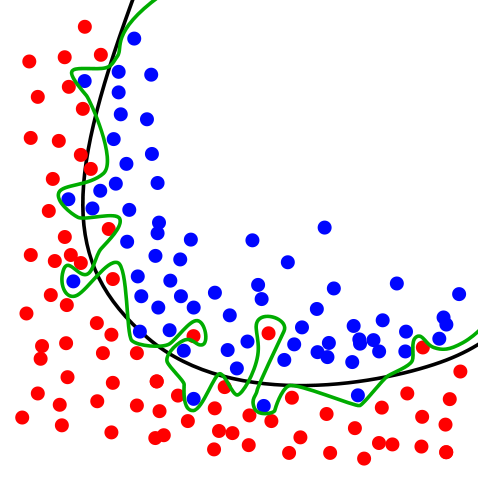
\includegraphics[width=0.4\linewidth]{images/Overfitting}
	\caption{An example of overfitting in the case of classification. The objective is to separate blue points from red points. Black line shows a classifier $f_1$ with low complexity where as green line illustrates a classifier $f_2$ with high complexity. On training examples (blue and red points), the model $f_2$ separates all the classes perfectly but may lead to poor generalization on new unseen examples. Model $f_1$ is often preferred.}
	\label{fig:Overfitting}
\end{figure}

In most cases, learning algorithms require to tune some hyper-parameters. A first approach could consists in trying all the possible combinations of hyper-parameters values and keep the one with the lowest training error. However, as discussed above, the model with the lowest training error is not always the one with the best generalization error.  To avoid overfitting, the training set can be divided into 2 sets: a learning and a validation set. Suppose we have two hyper-parameters to tune: $C$ and $\gamma$. We make a grid search for each combination $(C,\gamma)$ of the hyper-parameters, that is in this case a 2-dimensional grid (Fig. \ref{fig:GridSearch}). For each combination (a cell of the grid), the model is learnt on the learning set and evaluated on the validation set. At the end, the model with the lowest error on the validation set is retained. This process is referred as the model selection. 

\begin{figure}[h!]
	\centering
	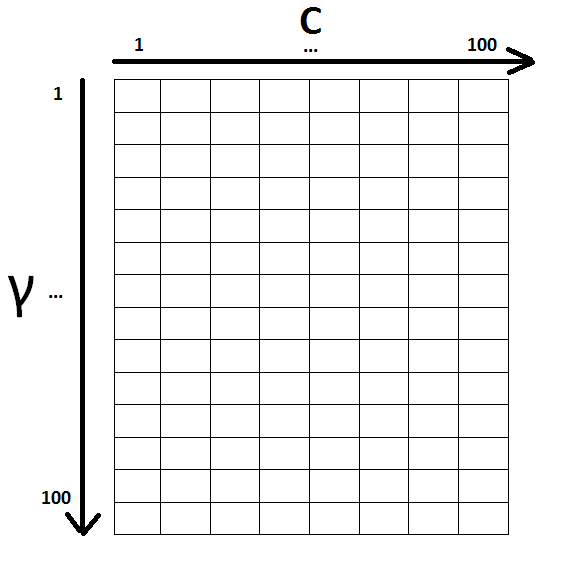
\includegraphics[width=0.4\linewidth]{images/GridSearch}
	\caption{Example of a 2 dimensional grid search for parameters $C$ and $\gamma$. It defines a grid where each cell of the grid contains a combination ($C$, $\gamma$). Each combination is used to learn the model and is evaluated on the validation set.}
	\label{fig:GridSearch}
\end{figure}

\begin{figure}[h!]
	\centering
	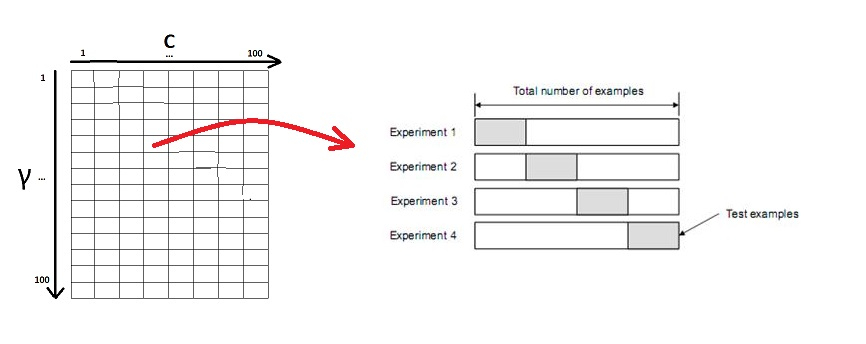
\includegraphics[width=1\linewidth]{Cross_validation2}
	\caption{$v$-fold Cross-validation for one combination of parameters. For each of $v$ experiments, use $v-1$ folds for training and a different fold for Testing, then the training error for this combination of parameter is the mean of all testing errors. This procedure is illustrated for $v=4$.}
	\label{fig:Cross_validation}
\end{figure}

An alternative is cross-validation with $v$ folds, illustrated in Fig. \ref{fig:Cross_validation}. In this approach, we partition the training data into $v$ equal-sized subsets. The objective is to evaluate the error for each combination of hyper-parameters. For each run, one fold is chosen for validation, while the $v-1$ remaining folds are used as the learning set. We repeat the process for each fold, thus $v$ times. Each fold gives one validation error and thus we obtain $v$ errors. The total error for the current combination of hyper-parameters is obtained by summing up the errors for all $v$ folds. When $v=n$, the size of training set, this approach is called leave-one-out or Jackknife. Each test set contains only one sample. The advantage is that as much data as possible are used for training. Moreover, the validation sets are exclusive and they cover the entire data set. The drawback is that it is computationally expensive to repeat the procedure $n$ times. Furthermore, since each validation set contains only one record, the variance of the estimated performance metric is usually high. This procedure is often used when $n$, the size training set, is small. There exists other methods such as sub-sampling or bootstraps \cite{Duda1973,Dreyfus2006}. We only use cross-validation in our experiments.

\noindent To sum up, Fig. \ref{fig:LearningFramework} shows a general approach for solving machine learning problems. In general, a dataset can be divided into 3 sub-datasets (illustrated in Fig. \ref{fig:Dataset}):
\begin{itemize}
	\item A \textbf{training set} $X=\{\textbf{x}_i,y_i\}_{i=1}^n$, which consists of $n$ samples $\textbf{x}_i$ whose labels $y_i$ are known. The training set is used to build the supervised model $f$. When the learning algorithm requires some hyper-parameters to be tuned, there exists a risk of model overfitting. To avoid such risks, the training set $X$ has to be divided into two subsets :
	\begin{itemize}
		\item A \textbf{learning set} which is used to build the supervised model $f$ for each value of the hyper-parameters.
		\item A \textbf{validation set} which is used to evaluate the supervised model $f$ for each value of the hyper-parameter. The model $f$ with the lowest error on the validation set is kept, thus ensuring that it has the best generalization abilities.
	\end{itemize}
	\item A \textbf{test set} $X_{Test}=\{\textbf{x}_j,y_j\}_{j=1}^m$, which consists of $m$ samples $\textbf{x}_j$ whose labels $y_j$ are also known but are not used during the training step. The model $f$ is applied to predict the label $\hat{y_j}$ of samples $\textbf{x}_j$ to evaluate the performance of the learnt model by comparing $\hat{y_j}$ and $y_j$. 
	\item An \textbf{operational set} $X_{op}=\{\textbf{x}_l,y_l\}_{l=1}^L$, which consists of $L$ samples $\textbf{x}_l$ whose labels $y_l$ are totally unknown. The operational set is in general a new dataset on which the learnt algorithm is applied. 
\end{itemize}


\begin{figure}[h!]
	\centering
	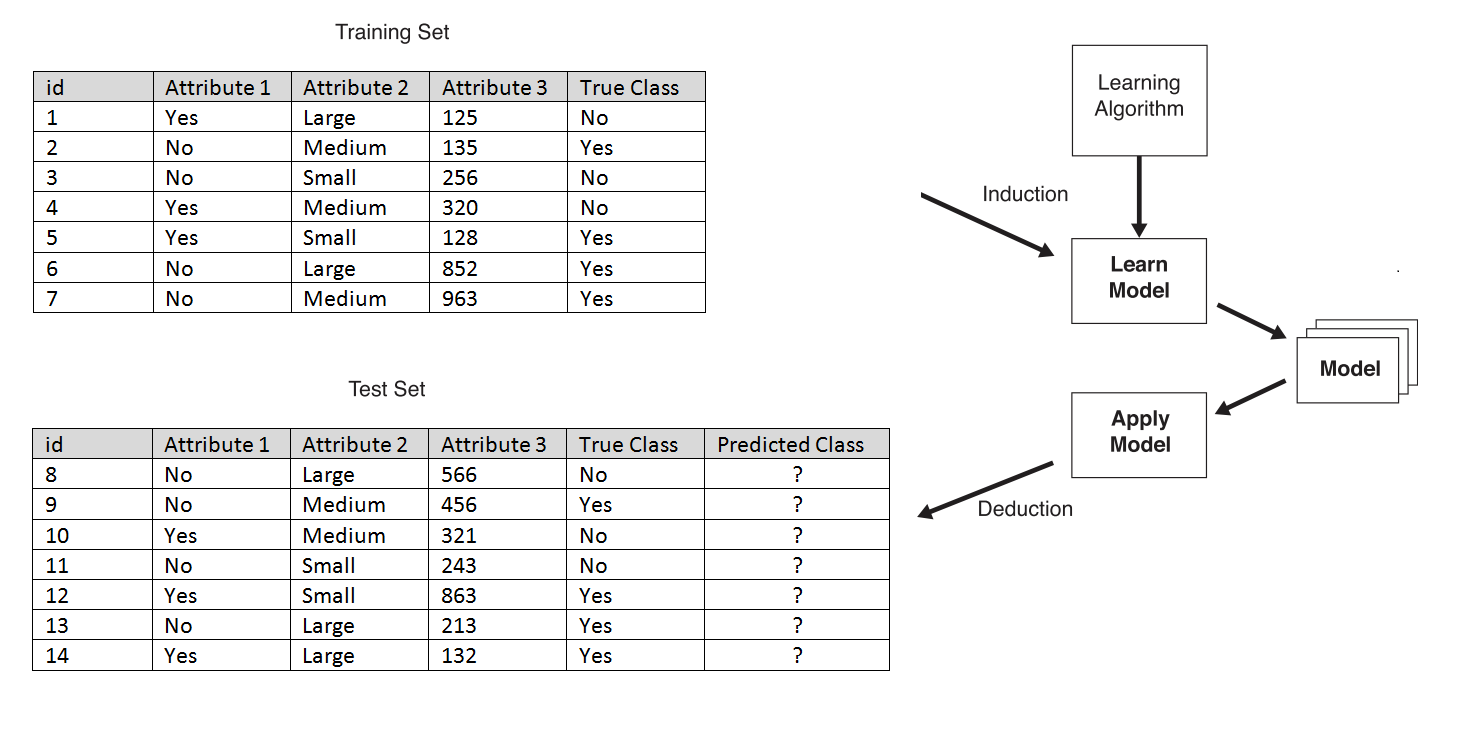
\includegraphics[width=1\linewidth]{images/LearningFramework}
	\caption{General framework for building a supervised (classification/regression) model. Example with 3 features and 2 classes ('Yes' and 'No').}
	\label{fig:LearningFramework}
\end{figure}

\begin{figure}[h!]
	\centering
	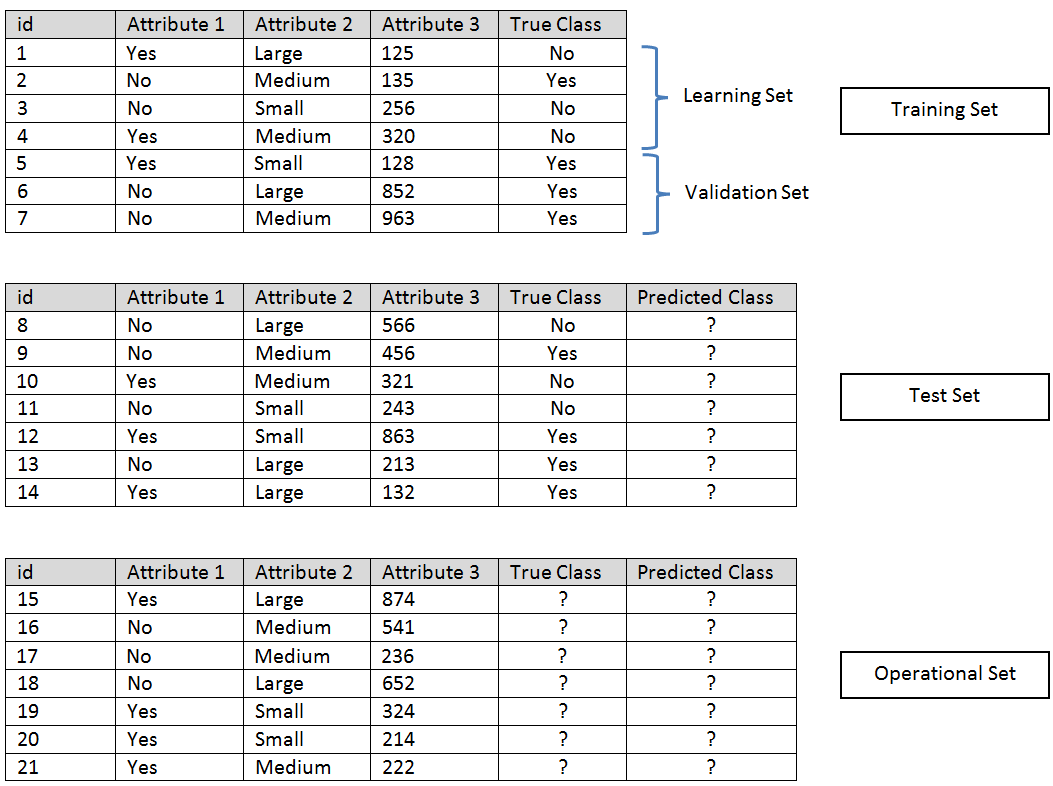
\includegraphics[width=0.9\linewidth]{images/Dataset}
	\caption{Division of a dataset into 3 datasets: training, test and operational.}
	\label{fig:Dataset}
\end{figure}

%\mycomment[MR]{refaire cette partie là} First, a training set $X=\{(\textbf{x}_i,y_i)\}_{i=1}^n$ consisting of $m$ samples $\textbf{x}_i$ whose labels $y_i$ are known is provided. The training set is used to build the supervised model $f$. Then, the model is applied to the test set $X_{Test}=\{(\textbf{x}_j,y_j)\}_{j=1}^m$, which consists of samples $\textbf{x}_j$ with unknown labels $y_j$. The test is used to evaluate the performance of the learnt model. 



\newpage
\subsection{Model evaluation}
%\begin{itemize}
%	\item Classification Error et test de significativité
%	\item Regression Error
%\end{itemize}

As seen in the previous section, model selection is inherently based on the ability to quantify its error on the training and validation sets. In this section, we recall how this error is computed for classification and regression problems.

\subsubsection{Classification evaluation}
\label{sec:ClassificationEvaluation}
The performance of a classification model is based on the counts of test samples $\textbf{x}_j$ correctly and incorrectly predicted by the model $f$. These counts are tabulated in a table called the confusion matrix. Table \ref{fig:ConfusionMatrix} illustrates the concept for a binary classification problem. Each cell $g_{ij}$ of the table stands for the number of samples from class $i$ predicted to be of class $j$. Based on this matrix, the number of correct predictions made by the model is $\sum_{i=1}^C g_{ii}$, where $C$ is the number of classes. % Equivalently, the ratio of incorrect predictions is $1-\sum_{i=1}^C g_{ii}$.

\begin{table}[h!]
	\centering
	\begin{tabular}{|c|c|c|c|}
		\hline      &  & \multicolumn{2}{c|} {Predicted class } \\ 
		\cline{3-4} &  & Class = 1 & Class = 0  \\ 
		\hline  \multirow{2}{*}{Actual Class } & Class = 1  & $g_{11}$ & $g_{10}$ \\ 
		\cline{2-4}  & Class = 0  & $g_{01}$ & $g_{00}$ \\ 
		\hline 
	\end{tabular}
	\caption{Confusion matrix for a 2-class problem.} 
	\label{fig:ConfusionMatrix}
\end{table}

\noindent For binary classification problems, $g_{11}$ is the number of true positives, $g_{10}$ is the number of false negatives, $g_{01}$ is the number of false positives and $g_{00}$ is the number of true negatives.

To summarize the information, it generally more convenient to use performance metrics such as the classification accuracy ($Acc$) or error rate ($Err$). This allows to compare several models with a single number. Note that $Err = 1-Acc$.
\begin{align}
Acc & = \frac{\text{Number of correct predictions}}{\text{Total number of predictions}} = \frac{\sum\limits_{i=1}^{C} g_{ii}}{\sum\limits_{i,j=1}^{C} g_{ij}} \\
Err & = \frac{\text{Number of wrong predictions}}{\text{Total number of predictions}} = \frac{\sum\limits_{i,j=1, i \neq j}^{C} g_{ij}}{\sum\limits_{i,j=1}^{C} g_{ij}}
\end{align}

Using these performance metrics allows to compare the performance of different classifiers $f$. It allows to determine in particular whether one learning algorithm outperforms another on a particular learning task on a given test dataset $X_{Test}$. However, depending on the size of the test dataset, the difference in error rate $Err$ between two classifiers may not be statistically significant. Snedecor \& Cochran proposed in 1989 a statistical test based on measuring the difference between two learning algorithms \cite{Cochran1977}. It has been used by many researchers \cite{Dietterich1997,Dietterich1995}.

Let consider 2 classifiers $f_A$ and $f_B$. We test these classifiers on the test set $X_{Test}$ and denote $p_A$ and $p_B$ their respective error rates. The intuition of this statistical test is that when algorithm A classifies an example $\textbf{x}_j$ from the test set $X_{Test}$, the probability of misclassification is $p_A$. Thus, the number $m_A$ (resp. $m_B$) of misclassification of $m$ test examples made by classifier $f_A$ (resp. $f_B$) is a binomial random variable with mean $mp_A$ and variance $p_A(1-p_A)m$. The binomial distribution can be approximated by a normal distribution when $m$ has a reasonable value (Law of large numbers). The difference between two independent normally distributed random variables is also normally distributed with a mean $m(p_A-p_B)$. Thus, the quantity $m_A-m_B$ is a normally distributed random variable. Under the null hypothesis (the two algorithm should have the same error rate), this will have a mean of zero and a standard error $se$ of:
\begin{equation}
se = \sqrt{\frac{2p(1-p)}{m}}
\end{equation}
\noindent where $p=\frac{p_A+p_B}{2}$ is the average of the two error probabilities. From this analysis, we obtain the statistic:
\begin{equation}
z=\frac{p_A-p_B}{\sqrt{2p(1-p)/m}}
\end{equation}
\noindent which has (approximatively) a standard normal distribution. We can reject the null hypothesis if $|z| > Z_{0.975} = 1.96$ (for a 2-sided test with probability of incorrectly rejecting the null hypothesis of 0.05).


\subsubsection{Regression evaluation}
As the concept of classes is restricted to classification problems, the performance of a regression model $f$ is based on metrics that measure the difference between the predicted label $\hat{y}_j$ and the known label $y_j$. The Mean Absolute Error function ($MAE$) computes the mean absolute error, a risk metric corresponding to the expected value of the absolute error loss or $L_1$-norm loss.

\begin{equation}
MAE = \frac{1}{m} \sum_{j=1}^m|\hat{y}_j-y_j|
\end{equation}

A commonly used performance metrics is the Root Mean Squared Error function ($RMSE$) that computes the root of the mean square error, a risk metric corresponding to the expected value of the squared (quadratic) error loss.

\begin{equation}
RMSE = \sqrt{\frac{1}{m} \sum_{j=1}^m(\hat{y}_j-y_j)^2}
\end{equation}

Many works rely on the $R^2$ function, the coefficient of determination. It provides a measure of how well future samples are likely to be predicted by the model \footnote{\url{http://scikit-learn.org/stable/modules/model_evaluation.html}}. It can also be interpreted as a measure of how the model $f$ is better than a constant model \todo{ref sylvain?}. 

\begin{equation}
R^2 = 1- \frac{\sum_{j=1}^m (\hat{y}_j-y_j)^2}{\sum_{j=1}^m (\bar{y}-y_j)^2}
\end{equation}

\noindent where $\bar{y} = \sum_{j=1}^m y_j$ is the mean over the known labels $y_j$.


\subsection{Data normalization}
\label{sec:data_normalization}
Real dataset are often subjected to noise or uneven scaling. Before applying any learning protocol, it is often necessary to pre-process the data: data scaling, data filtering (e.g., de-noising), outlier removal, etc. We focus on data normalization (data scaling) in our work.

Part 2 of Sarle's Neural Networks FAQ (1997) \footnote{\url{http://www.faqs.org/faqs/ai-faq/neural-nets/}} explains the importance of data normalization for neural networks but they can be applied to any learning algorithms. The main advantage of normalization is to avoid attributes in greater numeric ranges to dominate those in smaller numeric ranges. Another advantage is to avoid numerical difficulties during the calculation. For example, in the case of Support Vector Machine ({\sc svm}), because kernel values usually depend on the inner products of feature vectors, i.e. the linear kernel and the polynomial kernel, large attribute values might cause numerical problems \cite{Hsu2008}. 

In most cases, it is recommended to scale each attribute to the range [-1; +1] or [0; 1]. Many normalization methods have been proposed such as Min/Max normalization, Z-normalization or normalization of the log distribution \todo{références normalization}. Let $X=\{\textbf{x}_i,y_i\}_{i=1}^n$ be a training set, $\textbf{x}_i$ being a sample described by $p$ features $x_1, \ldots, x_p$. We define $\mu_j$ and $\sigma_j$ as the mean and the standard deviation of a variable $x_j$, applying the Z-normalized variable $x^{norm}_j$ is given by:
\begin{equation}
x^{norm}_j = \frac{x_j-\mu_j}{\sigma_j}
\end{equation}
Note that the underlying assumption supposes that the variable $x_j$ is normally distributed: data evolves between $[-\infty;+\infty]$ and are coming from a Gaussian process. In some cases, the data are skewed such as monetary amounts or incomes. These data are sometimes log-normally distributed, e.g., the log of the data is normally distributed (Fig. \ref{fig:SkewedData}). The underlying idea is to take the log of the data ($x^{ln}_j$) to restore the symmetry, and then, to apply a Z-normalization of this transformation:
\begin{align}
x^{ln}_j 		& = \ln(x_j); \\
x^{ln,norm}_j & = \frac{x^{ln}_j-\mu^{ln}_j}{\sigma^{ln}_j} \\
x^{norm}_j 	& = \exp(x^{ln,norm}_j)
\end{align}

\noindent where $\ln$ denotes the Natural Logarithm function, $\mu^{ln}_j$ and $\sigma^{ln}_j$ the mean and the standard deviation of a variable $x^{ln}_j$.

\begin{figure}
	\centering
	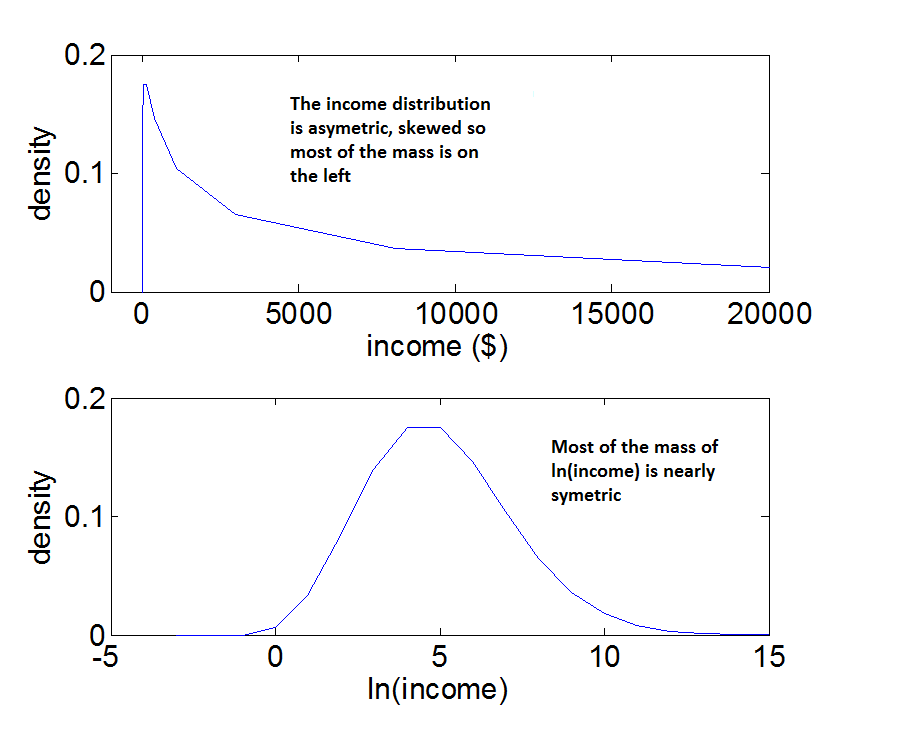
\includegraphics[width=0.6\linewidth]{images/SkewedData2}
	\caption{A nearly log-normal distribution, and its log transform \protect\footnotemark}
	\label{fig:SkewedData}
\end{figure}
\footnotetext{source: \url{http://www.r-statistics.com/2013/05/log-transformations-for-skewed-and-wide-distributions-from-practical-data-science-with-r/}}

Finally, we recall some precautions to the practitioner in the learning protocol, experimented by Hsu \& al. in the context of {\sc svm} \cite{Hsu2008}. First, training and testing data must be scaled using the same method. Second, training and testing data must not be scaled separately. Third, the whole dataset must not be scaled together at the same time. These often leads to poorer results. A proper way to do normalization is to scale the training data, store the parameters of the normalization (e.g. $\mu_i$ and $\sigma_i$ for Z-normalization), then apply the same normalization to the testing data. 


%------------------------------------------------------------------------------
\newpage
\section{Machine learning algorithms}

\mycomment[AD]{dit d'enlever 1ère phrase mais Michèle dit de garder}Many algorithms have been proposed in the context of supervised learning, such as Deep Neural Networks, Decision Trees or Relevance Vector Machines ({\sc rvm}). Our proposition relies on both results from Support Vector Machines ({\sc svm}) in the context of $k$-Nearest Neighbors ($k$-NN) classification. We limit the section to present these two algorithms. 
% We focus on $k$-Nearest Neighbors ($k$-NN) and Support Vector Machine ({\sc svm}). % The interest of these two is that they are based on the comparison of samples (time series in our case) through a distance measure, notion detailed in the next chapters.  

% We are going to detail now a few number of machine learning algorithms used classically to solve classification or regression problems. Other algorithms are popular nowadays such as Deep neural network, Decision tree or Relevance vector machine. We focus on $k$-Nearest Neighbors ($k$-NN) and Support Vector Machine ({\sc svm}) because these algorithms are based on the comparison of samples (time series in our case) through a distance measure, notion detailed in the next chapters.

\subsection{$k$-Nearest Neighbors ($k$-NN) classifier}
\label{sec:kNN}
%\begin{itemize}
%	\item Donner l'intuition
%	\item Formaliser le problème en tant que problème d'optimisation
%	\item Présenter les extensions (kNN pondéré), extension à la régression
%	\item Soulever le fait que la résolution du problème fait intervenir une notion de distance entre les individus (time series)	
%	\item Donner les arguments qui permettent de dire pourquoi utiliser un 1-NN permet de faire une évaluation de métriques (Ding)
%\end{itemize}

\mycomment[AR]{Ahlame trouve que ce n'est pas clair. A refaire}A simple approach to classify samples is to consider that "close" samples have a great probability to belong to the same class. Given a test sample $\textbf{x}_j$, one can use the class $y_i$ of its nearest neighbor $\textbf{x}_i$ in the training set in order to predict its labels: $\hat{y}_j=y_i$. \\
\indent More generally, we can consider the $k$ nearest neighbors of $\textbf{x}_j$. The class $y_j$ of a test sample $\textbf{x}_j$ is assigned with a voting scheme among them, i.e., using the majority of the class of nearest neighbors. This algorithm is referred as the $k$-Nearest Neighbors algorithm ($k$-NN) 
\cite{Silverman1989,Cover1967b}. Fig. \ref{fig:kNN_example} illustrates the concept for a neighborhood of $k=3$ and $k=5$.

\begin{figure}[h!]
\centering
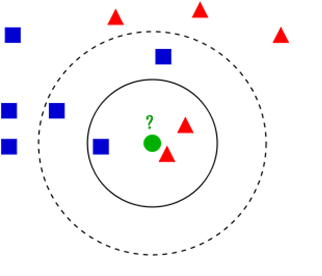
\includegraphics[width=0.40\linewidth]{images/kNN_example}
\caption{Example of $k$-NN classification. The test sample (green circle) is classified either to the first class (red stars) or to the second class (blue triangles). If $k = 3$ (solid line circle) it is assigned to the second class because there are 2 triangles and only 1 star inside the inner circle. If $k = 5$ (dashed line circle) it is assigned to the first class (3 stars vs. 2 triangles inside the outer circle).}
\label{fig:kNN_example}
\end{figure}

\indent In the $k$-NN algorithm, the notion of "closeness" between samples $\textbf{x}_i$ is based on the computation of a metric \footnote{A clarification of the terms metric, distance, dissimilarity, etc. will be given in Chapter \ref{sec:Chapter_metrics}. For now, we refer all of them as metrics.} $D$. For static data, frequently used metrics are the Euclidean distance, the Minkowski distance or the Mahalanobis distance. Considering a training set $X$ of $n$ samples, solving the 1-NN classification problem is equivalent to solve the following optimization problem: for a new sample $\textbf{x}_j$, $\forall i \in \{1...n\}$,
\begin{equation}
y_j = y_{i^*}
\end{equation}
where $i^*={\underset{i \in \{1...n\}}{\argmin}   D(\textbf{x}_i,\textbf{x}_j)}$.

The $k$-NN algorithm can be extended to estimate continous labels (regression problems). The procedure is similar. The label $y_j$ is defined as :
\begin{equation}
y_j = \frac{1}{k}\sum_{i=1}^{k} y_{i}
\end{equation}
where $i$ corresponds to the index of the $k$-nearest neighbors \cite{Altman1992}. There exists other variants of the $k$-NN algorithms. In a weighed $k$-NN, the approach consists in weighting the $k$-NN decision by assigning to each neighbor $\textbf{x}_i$ from an unknown sample $\textbf{x}_j$, a weight $w_i$ defined as a function of the distance $D(\textbf{x}_i, \textbf{x}_j)$ \cite{Dudani1976}. To cope with uncertainty or imprecision in the labeling of the training data $\textbf{x}_i$, other authors propose in a fuzzy $k$-NN to determine the membership degree in each class of an unseen sample $\textbf{x}_j$ by combining the memberships of its neighbors \cite{Keller1985}. \mycomment[AD]{Expliquer d'avantage} Denoeux propose a framework based on Dempster-Shafer theory where the $k$-NN rule takes into account the non-representativity of training data, the weighting rule and uncertainty in the labeling \cite{Denoeux1995}.

% in weighting each neighbors labels $y_{i}$ by a factor equal to the inverse of the distance $\frac{1}{D(\textbf{x}_i, \textbf{x}_j)}$ \cite{Dudani1976}. To cope with uncertainty or imprecision in the labelling of the training data, some authors propose in a fuzzy $k$-NN to determine the membership degree of an unseen pattern in each class by combining the memberships of its neighbors. assign a degree of membership of a training vector $\textbf{x}_i$ memberships of samples $\textbf{x}_j$ to classes. in a fuzzy $k$-NN, the idea is to assign memberships of samples $\textbf{x}_j$ to classes. The class membership is a function of the sample’s distance $D(\textbf{x}_i, \textbf{x}_j)$ from its $k$-NN training samples\todo{[biblio fuzzy kNN]}; in a credibilist $k$-NN\mycomment[MR]{+ $k$-NN crédibiliste} \cite{Denoeux1995}

Despite its simplicity, the $k$-NN algorithm has been shown to be successful on time series classification problems \cite{Belongie2002,Xi2006a,Ding2008}. 
%presents many advantages and
% \mycomment[AD]{Ahlame trouve que le discours s'éloigne et on devrait supprimer jusqu'à la fin des avantages}One main advantage is that a 1-NN classifier can be used to evaluate and compare the efficiency of different metrics \cite{Ding2008}. First, the underlying metric is critical in the performance of the 1-NN classifier \cite{Tan2005b}. Thus, the accuracy of the 1-NN classifier directly reflects the effectiveness of the metric. Second, 1-NN classifier is easy to implement and doesn't need to learn any hyper-parameters, which make it straightforward for anyone to reproduce results. All of this advantages allows one who want to evaluate a benchmark of metrics. Other methods to compare metrics exists such as clustering with small data sets which are not statistically significant, or compare the compactness of the metric \cite{Morse2007,Vlachos2006}. The 1-NN algorithm will be used in our experiments to compare the performances different metrics used for time series.
However, the $k$-NN algorithm presents some disadvantages, mainly due to its computational complexity, both in memory space (storage of the training samples $\textbf{x}_i$) and time (search of the neighbors) \cite{Duda1973}. Suppose that we have $n$ labeled training samples in $p$ dimensions, and find the closest neighbors to a test sample $\textbf{x}_j$ ($k = 1$). In the most simple approach, we look at each stored samples $\textbf{x}_i$ ($i=1...n$) one by one, calculate its distance to $\textbf{x}_j$ (D($\textbf{x}_i$,$\textbf{x}_j$)) and retain the index of the current closest one. For the standard Euclidean distance, each metric computation is $O(p)$ and thus the search is $O(pn)$. Finally, note that using standard metrics (such as the Euclidean distance) in the $k$-NN relies on all $p$ dimensions in its computation and thus assumes that all dimensions have the same effect on the metric. This assumption may be wrong and can impact the classification performances. 
%The importance of defining adapted metrics for time series will be discussed in Chapter \ref{sec:Chapter_metrics}.


% \textcolor{red}{Accuracy evaluation answers one of the most important questions about a similarity measure: why is this a good measure for describing the (dis)similarity between time series? Surprisingly, we found that accuracy evaluation is usually insufficient in existing literature: it has been either based on subjective evaluation, e.g., [4, 9], or using clustering with small data sets which are not statistically significant, e.g., [31, 40]. In this work, we use an objective evaluation method recently proposed [25]. The idea is to use a one nearest neighbor (1NN) classifier [17, 32] on la- belled data to evaluate the efficacy of the distance measure used. Specifically, each time series has a correct class label, and the classifier tries to predict the label as that of its nearest neighbor in the training set. There are several advantages with this approach. First, it is well known that the underlying distance metric is critical to the performance of 1NN classifier [32], hence, the accuracy of the 1NN classifier directly reflects the effectiveness of the similarity measure. Second, the 1NN classifier is straightforward to implement and is parameter free, which makes it easy for anyone to reproduce our results. Third, it has been proved that the error ratio of 1NN classifier is at most twice the Bayes error ratio [36]. Finally, we note that while there have been attempts to classify time series with decision trees, neural networks, Bayesian networks, supporting vector machines etc., the best published results (by a large margin) come from simple nearest neighbor methods [42]}

% Cons of the kNN
%Curse of Dimensionality
%* Distance usually relates to all the attributes and assumes all
%of them have the same effects on distance
%* The similarity metrics do not consider the relation of
%attributes which result in inaccurate distance and then impact
%on classification precision. Wrong classification due to
%presence of many irrelevant irrelevant attributes attributes is often termed as the
%curse of dimensionality
%* For example: Each instance is described by 20 attributes out
%of which only 2 are relevant in determining the classification
%of the target function. In this case, instances that have
%identical values for the 2 relevant attributes may
%nevertheless be distant from one another in the 20
%dimensional instance space
%(http://www.csee.umbc.edu/~tinoosh/cmpe650/slides/K_Nearest_Neighbor_Algorithm.pdf)


\subsection{Support Vector Machine ({\sc svm}) algorithm}
%\begin{itemize}
%	\item Présenter le principe général des {\sc svm} en commençant par l'intuition.
%	\item Forme primale: donner la formulation primale du problème d'optimisation
%	\item Forme duale: montrer commencer passer de la forme primal à la forme dual.
%	\item A partir de la forme duale, passer au kernel
%	\item Finir par la complexité du {\sc svm} en apprentissage ($o(N^3p)$) et en test (limités aux nombres de support vectors) et les interprétations des supports vectors.
%	\item Expliquer la modification du problème initiale avec une régularisation $L_1$ sur le terme de régularisation et nous permet d'avoir une solution sparse (donner 1 cas où la solution sparse est meilleur).
%	\item Expliquer que dans le cadre de données non-balancées, il faut ajouter des termes pour rebalancer l'équation du {\sc svm}
%\end{itemize}

Support Vector Machine ({\sc svm}) is a classification method introduced in 1992 by Boser, Guyon, and Vapnik \cite{Boser1992,Cortes1995} to solve at first linearly separable problems. The {\sc svm} classifier has demonstrated high accuracy, ability to deal with high-dimensional data, good generalization properties and interpretation for various applications from recognizing handwritten digits, to face identification, text categorization, bioinformatics and database marketing \cite{Wang2002,Yang1999,Heisele2001,Sadri2003,Campbell2011}. {\sc svm}s belong to the category of kernel methods, algorithms that depends on the data only through dot-products \cite{Schlkopf2013}. It allows thus to solve non-linear problems. This section gives a brief overview of the mathematical key points and interpretation of the method. For more informations, the reader can consult \cite{Schlkopf2013,Campbell2011,Cortes1995}.

We first present an intuition of maximum margin concept. We give the primal formulation of the {\sc svm} optimization problem. Then, by transforming the latter formulation into its dual form, the kernel trick can be applied to learn non-linear classifiers. Finally, we detail how we can interpret the obtained coefficients and how {\sc svm}s can be extended for regression problems.



\subsubsection{Intuition}
\mycomment[AD]{Mettre dans les figures des + et - pour les classes}Let $\{\textbf{x}_i,y_i\}_{i=1}^n$ be a set of $n$ samples $\textbf{x}_i \in \mathbb{R}^p$ and their labels $y_i= \pm 1$ (2 class-problem). The objective is to learn a hyperplane, whose equation is $\textbf{w}^T \textbf{x} + b = 0$, that can separate samples of class +1 from the ones of class -1. When the problem is linearly separable such as in Fig. \ref{fig:Plusieurs_separatrice_lineaire}, there exists an infinite number of valid hyperplanes. 

\begin{figure}[h!]
\centering
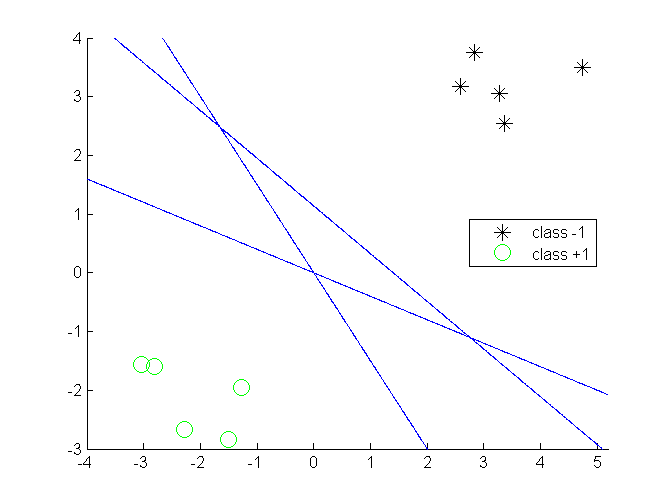
\includegraphics[width=0.5\linewidth]{images/Plusieurs_separatrice_lineaire2}
\caption{Example of linear classifiers in a 2-dimensional classification problem. For a set of points of classes +1 and -1 that are linearly separable, there exists an infinite number of separating hyperplanes corresponding to $\textbf{w}^T\textbf{x} + b = 0.$ }
\label{fig:Plusieurs_separatrice_lineaire}
\end{figure}

\noindent Vapnik \& al. \cite{Cortes1995} propose to choose the separating hyperplane that maximizes the margin, e.g. the hyperplane that leaves as much distance as possible between the hyperplane and the closest samples $\textbf{x}_i$ of each class, called the support vectors. This distance is equal to $\frac{1}{||\textbf{w}||_2}$. We denote $||\textbf{w}||_2$, the $L_2$-norm of the vector $\textbf{w}$ and $||\textbf{w}||_1$ the $L_1$-norm of $\textbf{w}$:
\begin{align}
	||\textbf{w}||_2 & = \sqrt{\textbf{w}^T \textbf{w}} = \sqrt{\sum\limits_{h=1}^{p} w_h^2}\\
	||\textbf{w}||_1 & = \sum\limits_{h=1}^{p} |w_h|
\end{align}
\noindent where $\textbf{w} = [w_1, \ldots, w_p]^T$ denotes the weight vector. \\
The two hyperplanes passing through the support vectors of each class are referred as the canonical hyperplanes, and the region between the canonical hyperplanes is called the margin band (Fig. \ref{fig:Separatrice_lineaire_avec_marges}). From this, for a binary classification problem, to classify a new sample $\textbf{x}_j$, the decision function is:
\begin{equation}
f(\textbf{x}_j) = sign(\textbf{w}^T \textbf{x}_j + b) \label{eq:decision_function}
\end{equation}

\begin{figure}
\centering
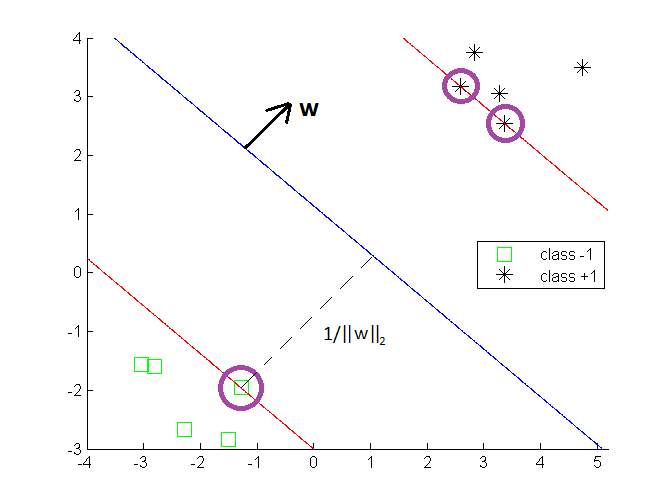
\includegraphics[width=0.6\linewidth]{images/Separatrice_lineaire_avec_marges2}
\caption{The argument inside the decision function of a classifier is $\textbf{w}^T\textbf{x} + b$. The separating hyperplane corresponding to $\textbf{w}^T\textbf{x} + b = 0$ is shown as a line in this 2-dimensional plot. This hyperplane separates the two classes of data with points on one side labeled $y_i = +1$ ($\textbf{w}^T\textbf{x}_i + b \geq 0$) and points on the other side labeled $y_i=-1$ ($\textbf{w}^T\textbf{x}_i + b < 0$). Support vectors are circled in purple and lies on the hyperplanes $\textbf{w}^T\textbf{x} + b = +1$ and $\textbf{w}^T\textbf{x} + b = -1$}
\label{fig:Separatrice_lineaire_avec_marges}
\end{figure}

% \missingfigure{Make a figure with many hyperplans. Put the one that maximize the hyperplan between the support vectors. Example of caption: }



\subsubsection{Primal formulation}
Finding $\textbf{w}$ and $b$ by maximizing the margin $\frac{1}{||\textbf{w}||_2}$ is equivalent to minimizing the norm of $\textbf{w}$ such that all samples from the training set are correctly classified:
	\begin{align}
		& \argmin_{\textbf{w},b} \frac{1}{2} ||\textbf{w}||_2^2 \label{eq:objectiveSVM}\\
		& \textbf{s.t. } y_i(\textbf{w} ^T\textbf{x}_i+b) \geq 1 \label{eq:constraintsSVM}
	\end{align}
This is a constrained optimization problem in which we minimize an objective function (Eq. \ref{eq:objectiveSVM}) subject to constraints (Eq. \ref{eq:constraintsSVM}). This formulation is referred as the primal hard margin problem. When the problem is not linearly separable, slack variables $\xi_i \geq 0$ are introduced to relax the optimization problem:
	\begin{align}
	& \argmin_{\textbf{w},b, \xi}  
	\left( 
	\overbrace{\vphantom{\sum_{i=1}^n \xi_i}
		\frac{1}{2}||\textbf{w}||^2_2}^{Regularization}
	+ C \overbrace{\sum\limits_{i=1}^{n}\xi_i}^{Loss} \right) 
	\label{eq:objectiveSVM2}\\
	& \textbf{s.t. } y_i(\textbf{w}^T\textbf{x}_i+b) \geq 1 -\xi_i \label{eq:constraintsSVM2} \\
	&  \xi_i \geq 0 \label{eq:constraintsSVM20}
	\end{align}
\noindent where $C > 0$ is a penalty hyper-parameter. 
	
This formulation is referred as the primal soft margin problem. It is a quadratic programming optimization problem subjected to constraints. Thus, it is a convex problem: any local solutions is a global solution. The objective function in Eq.~\ref{eq:objectiveSVM2} is made of two terms. The first one, the regularization term, penalizes the complexity of the model and thus, controls the ability of the algorithm to generalize on new samples. The second one, the loss term, is an adaptation term to the data. The hyper-parameter $C$ is a trade-off between the regularization and the loss term. When $C$ tends to $+\infty$, all the slack variables $\xi_i$ have to be equal to zero for the loss not to be infinite. The problem is thus equivalent to the primal hard margin problem. The hyper-parameter $C$ is learnt during the training phase (Section \ref{sec:model_selection}). 


\subsubsection{Dual formulation}
\label{sec:dualSVM}
From the primal formulation, it is possible to have an equivalent dual form. This latter formulation allows samples $\textbf{x}_i$ to appear in the optimization problem through dot-products only. The kernel trick can be applied to extend the methods to learn non-linear classifiers.

First, to simplify the calculation development, let consider the hard margin formulation in Eqs. \ref{eq:objectiveSVM2}, \ref{eq:constraintsSVM2} and \ref{eq:constraintsSVM20}. As a constrained optimization problem, the formulation is equivalent to the minimization of a Lagrange function $L(\textbf{w},b)$, consisting of the sum of the objective function and the $n$ constraints multiplied by their respective Lagrange multipliers $\boldsymbol{\alpha} = [\alpha_1, \ldots, \alpha_n]^T$: 
\begin{align}
	& \argmax_{\boldsymbol{\alpha}} \left( L(\textbf{w},b) = \frac{1}{2}(\textbf{w}^T\textbf{w})-\sum\limits_{i=1}^{n}\alpha_i(y_i(\textbf{w}^T\textbf{x}_i+b)-1) \right) \label{eq:Lagrange} \\
	& \textbf{s.t. } \forall i = 1...n: \nonumber \\
	& \alpha_i \geq 0 \label{KKT1}\\
	& y_i(\textbf{w}^T\textbf{x}_i+b)-1 \geq 0 \label{KKT2}\\
	& \alpha_i (y_i(\textbf{w}^T\textbf{x}_i+b)-1) = 0 \label{KKT3}
\end{align}
\noindent where $\alpha_i \geq 0$ are the Lagrange multipliers. In optimization theory, Eq. \ref{KKT1}, \ref{KKT2} and \ref{KKT3} are called the Karush-Kuhn-Tucker ({\sc kkt}) conditions. It corresponds to the set of conditions which must be satisfied at the optimum of a constrained optimization problem. The {\sc kkt} conditions will play an important role in the interpretation of {\sc svm} in Section \ref{subsec:interpretation}. 

\noindent At the maximum value of $L(\textbf{w},b)$, we assume the derivatives with respect to $b$ and $\textbf{w}$ are set to zero:
\begin{align*}
\frac{\partial L}{\partial b} &= - \sum\limits_{i=1}^{n}\alpha_i y_i = 0 \\
\frac{\partial L}{\partial \textbf{w}} &= \textbf{w}-\sum\limits_{i=1}^{n}\alpha_i y_i \textbf{x}_i = 0
\end{align*}
\noindent that leads to:
\begin{align}
&\sum\limits_{i=1}^{n}\alpha_i y_i = 0 \\
& \textbf{w} = \sum\limits_{i=1}^{n}\alpha_i y_i \textbf{x}_i
\end{align}

\noindent By substituting $\textbf{w}$ into $L(\textbf{w},b)$ in Eq. \ref{eq:Lagrange}, we obtain the dual formulation (\textit{Wolfe dual}):
\begin{align}
	& \argmax_{\boldsymbol{\alpha}} \left( 
	\sum\limits_{i=1}^{n} \alpha_i - \frac{1}{2} \sum\limits_{i,j=1}^{n} \alpha_i \alpha_j y_i y_j (\textbf{x}_i ^T \textbf{x}_j) 
	\right) 
	\label{eq:dualSVM}\\
	& \textbf{s.t. } \forall i = 1...n: \nonumber \\
	& \sum\limits_{i=1}^{n}\alpha_i y_i = 0 \label{constraintdual1}\\
	& \alpha_i \geq 0 \label{constraintdual2}
\end{align}

\noindent The dual objective in Eq. \ref{eq:dualSVM} is quadratic in the parameters $\alpha_i$. Adding the constraints in Eqs. \ref{constraintdual1} and \ref{constraintdual2}, it is a constrained quadratic programming optimization problem ({\sc qp}). Note that while the primal formulation is minimization, the equivalent dual formulation is maximization. It can be shown that the objective functions of both formulations reach the same value when the solution is found \cite{Campbell2011}. \\
In the same spirit, considering the soft margin primal problem, it can be shown that it leads to the same formulation \cite{Campbell2011} (Eqs. \ref{eq:dualSVM} and \ref{constraintdual1}), except that 
the Lagrange multipliers $\alpha_i$ are upper bounded by the trade-off $C$ in the soft margin formulation:
\begin{align}
	& 0 \leq \alpha_i \leq C  \label{constraintdual4}
\end{align}
The constraints in Eq. \ref{constraintdual4} are called the Box constraints \cite{Campbell2011}. From the optimal value of $\alpha_i$, denoted $\alpha_i^*$, it is possible to compute the weight vector $\textbf{w}^*$ and the bias $b^*$ at the optimality:
\begin{align}
	\textbf{w}^* & = \sum\limits_{i=1}^{n}\alpha_i^* y_i \textbf{x}_i \label{eq:w_dual}\\
	b^* & = \sum\limits_{i=1}^{n} (\textbf{w}^T\textbf{x}_i - y_i)
\end{align}
At the optimality point, Eq. \ref{KKT3} leads $\alpha_i^* = 0$ for all datapoints that are well classified and that are not on the margin. Hence, only a few number of datapoints have $\alpha_i^* > 0$ as shown as in Fig. \ref{fig:SVM_SV}. These samples are the vector supports. All other datapoints have $\alpha_i^*=0$, and the decision function is independent of them. Thus, the representation is sparse. 

\noindent From Eqs. \ref{eq:decision_function} \& \ref{eq:w_dual}, to classify a new sample $\textbf{x}_j$, the decision function for a binary classification problem is:
\begin{equation}
	f(\textbf{x}_j) = sign(\sum\limits_{i=1}^{n} \alpha_i^*y_i(\textbf{x}_i^T\textbf{x}_j) + b^*) \label{decisionDual}
\end{equation} 

\begin{figure}[h!]
	\centering
	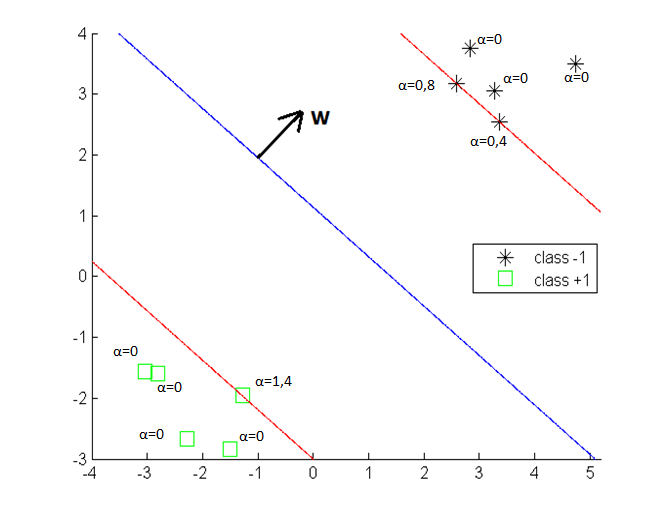
\includegraphics[width=0.6\linewidth]{images/SVM_SV2}
	\caption{Hyperplane obtained after a dual resolution (full blue line). The 2 canonical hyperplanes (red lines) contain the support vectors whose $\alpha_i > 0$. Other points have their $\alpha_i = 0$ and the equation of the hyperplane is only affected by the support vectors.}
	\label{fig:SVM_SV}
\end{figure}


\subsubsection{Kernel trick}
The concept of kernels was introduced by Aizerman \& al. in 1964 to design potential functions in the context of pattern recognition \cite{Aizerman1964}. The idea was re-introduced in 1992 by Boser \& al. for Support Vector Machine ({\sc svm}) and has been received a great number of improvements and extensions to symbolic objects such as text or graphs \cite{Boser1992}.

% One theoretical interesting property of {\sc svm} is that it has been shown that the generalization error bound does not depend on the dimensionality $p$ of the space \cite{Schlkopf2013}. 
From the dual objective in Eq. \ref{eq:dualSVM}, we note that the samples $\textbf{x}_i$ are only involved in a dot-product. Therefore, if we map these samples $\textbf{x}_i$ into a higher dimensional hyperspace, called the feature space, we only need to know the dot product in the feature space:
\begin{equation}
	(\textbf{x}_i . \textbf{x}_j) \rightarrow \Phi(\textbf{x}_i) . \Phi(\textbf{x}_j) 
\end{equation}
\noindent where $\Phi$ is the mapping function. \\

The intuition behind using such mapping is that for many datasets, it is not possible to find a hyperplan that can separate the two classes in the input space if the problem is not linearly separable. However, by applying a transformation $\Phi$, data might become linearly separable in a higher dimensional space. Fig. \ref{fig:SVM_nonlinear} illustrates the idea: in the original 2-dimensional space (left), the two classes can't be separated by a line. However, with a third dimension such that the $+1$ (circle) labeled points are moved forward and the $-1$ (cross) labeled moved back the two classes become separable.

In most of the case, the mapping function $\Phi$ does not need to be known since we only need the dot product $\Phi(\textbf{x}_i) . \Phi(\textbf{x}_j)$. Therefore, we can use any kernel function $K$ such that: $K(\textbf{x}_i,\textbf{x}_j)= \Phi(\textbf{x}_i) . \Phi(\textbf{x}_j)$. We call Gram matrix $G$, the matrix containing all $K(\textbf{x}_i,\textbf{x}_j)$:
\begin{equation*}
	G = (K(\textbf{x}_i,\textbf{x}_j))_{1 \leq i,j \leq n} = 
	\begin{pmatrix}
	K(\textbf{x}_1,\textbf{x}_1) & ... & K(\textbf{x}_1,\textbf{x}_n) \\
	... & & ... \\
	K(\textbf{x}_n,\textbf{x}_1) & ... & K(\textbf{x}_n,\textbf{x}_n) 
	\end{pmatrix}
\end{equation*}

\noindent Defining a kernel has to follow rules. One of these rules specifies that the kernel function has to define a proper inner product in the feature space. Mathematically, the Gram matrix has to be semi-definite positive (Mercer's theorem) \cite{Schlkopf2013}. These restricted feature spaces, containing an inner product are called Hilbert spaces.


\begin{figure}[h!]
\centering
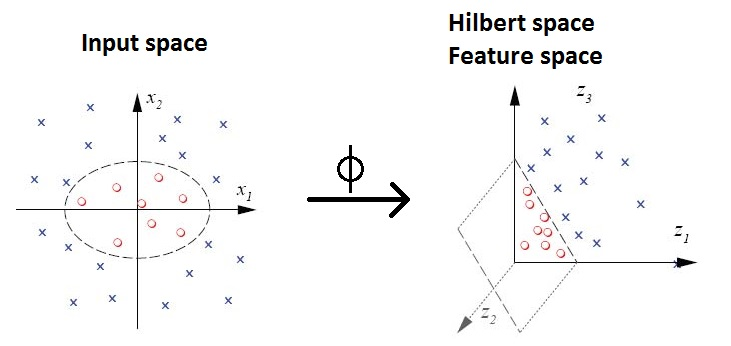
\includegraphics[width=0.9\linewidth]{images/SVM_nonlinear2}
\caption{Left: in two dimensions the two classes of data (-1 for cross and +1 for circle) are mixed together, and it is not possible to separate them by a line: the data is not linearly separable. Right: using a kernel, these two classes of data become separable by a hyperplane in feature space, which maps to the nonlinear boundary shown, back in input space.\protect\footnotemark}
\label{fig:SVM_nonlinear}
\end{figure}
\footnotetext{source: \url{http://users.sussex.ac.uk/~christ/crs/ml/lec08a.html}}

Many kernels have been proposed in the literature such as the polynomial, sigmoid, exponential or wavelet kernels \cite{Schlkopf2013}. The most popular ones that we will use in our work are respectively the Linear and the Gaussian (or Radial Basis Function ({\sc rbf})) kernels:
\begin{align}
	& K(\textbf{x}_i,\textbf{x}_j)= \textbf{x}_i ^T \textbf{x}_j \\
	& K(\textbf{x}_i,\textbf{x}_j)
	= \exp(-\frac{||\textbf{x}_j-\textbf{x}_i||_2^2}{2\sigma^2})
	= \exp(-\gamma||\textbf{x}_j-\textbf{x}_i||_2^2)
\end{align}
where $\gamma = \frac{1}{2\sigma^2}$ is the parameter of the Gaussian kernel and $||\textbf{x}_j-\textbf{x}_i||_2$ is the Euclidean distance between $\textbf{x}_i$ and $\textbf{x}_j$. Note that the Linear kernel is the identity transformation. In practice, for large scale problem (when the number of dimensions $p$ is high), using a Linear kernel is sufficient  \cite{Fan2008}.

The Gaussian kernel computed between a sample $\textbf{x}_j$ and a support vector $\textbf{x}_i$ is an exponentially decaying function in the input space. The maximum value of the kernel ($K(\textbf{x}_i,\textbf{x}_j)$=1) is attained at the support vector (when $\textbf{x}_i=\textbf{x}_j$). Then, the value of the kernel decreases uniformly in all directions around the support vector, with distance and ranges between zero and one. It can thus be interpreted as a similarity measure. Geometrically speaking, it leads to hyper-spherical contours of the kernel function as shown in Fig. \ref{fig:Kernel_Gaussian} \footnote{\url{https://www.quora.com/Support-Vector-Machines/What-is-the-intuition-behind-Gaussian-kernel-in-SVM}}. The parameter $\gamma$ controls the decreasing speed of the sphere. In practice, this parameter is learnt during the training phase.

\begin{figure}[h!]
\centering
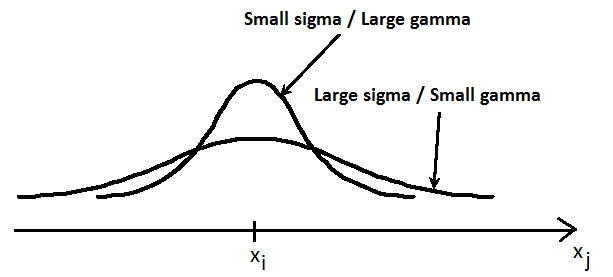
\includegraphics[width=0.6\linewidth]{images/Kernel_Gaussian2}
\caption{Illustration of the Gaussian kernel in the 1-dimensional input space for a small and large $\gamma$ when $\textbf{x}_i$ is fixed and $\textbf{x}_j$ varies.}
\label{fig:Kernel_Gaussian}
\end{figure}


By applying the kernel trick to the soft margin formulation in Eqs. \ref{eq:dualSVM}, \ref{constraintdual1} and \ref{constraintdual4}, the following optimization problem allows to learn non-linear classifiers:
\begin{align}
	& \argmax_{\boldsymbol{\alpha}} \left( 
	\sum\limits_{i=1}^{n} \alpha_i - \frac{1}{2} \sum\limits_{i=1}^{n} \sum\limits_{j=1}^{n} \alpha_i \alpha_j y_i y_j K(\textbf{x}_i , \textbf{x}_j) 
	\right) 
	\label{eq:dualSVM2kernel}\\
	& \textbf{s.t. } \sum\limits_{i=1}^{n}\alpha_i y_i = 0 \label{constraintdual3kernel}\\
	& 0 \leq \alpha_i \leq C  \label{constraintdual4kernel}
\end{align}

\noindent The decision function $f$ becomes:
\begin{equation}
f(\textbf{x}_j) = sign(\sum\limits_{i=1}^{n} \alpha_i^*y_i K(\textbf{x}_i,\textbf{x}_j) + b^*) \label{decisionDualKernel}
\end{equation} 
\noindent Let $n_{SV}$ be the number of support vectors ($n_{SV} \leq n$). To recover $b^*$, we recall that for support vectors $\textbf{x}_i$:
\begin{equation}
	y_j \left( \sum\limits_{i=1}^{n_{SV}} \alpha_i^* y_i K(\textbf{x}_i,\textbf{x}_j) + b^* \right) = 1
\end{equation}
From this, we can solve $b^*$ using an arbitrarily chosen support vector $\textbf{x}_i$:
\begin{equation}
	b^* = \frac{1}{y_j} - \sum\limits_{i=1}^{n_{SV}} \alpha_i^* y_i K(\textbf{x}_i,\textbf{x}_j)
\end{equation}
\noindent Note that in this case, we can't recover the weight vector $\textbf{w}^*$ but it is not useful here for the decision function.

\subsubsection{Interpretation}
\label{subsec:interpretation}
%\begin{itemize}
%	\item interpretation dans le primal: vecteur w et b
%	\item interpretation dans le dual
%	\item interpretation
%\end{itemize}

%\noindent \textbf{Complexity} \\
%\mycomment[CTD]{réécrire + compléter avec Claude}
%As the objective is to provide an algorithm for both small and large datasets, let us examine the complexity of {\sc svm}s and in the computation of the Gram matrix $G$ \cite{Bottou2007}.
%
%In the dual, suppose that we know which samples are not support vectors ($\alpha_i = 0$) and which sample are bounded support vectors ($\alpha_i = C$). The $R$ remaining support vectors are determined by a system of $R$ linear equations. They represent the derivatives of the objective function and requires a number of operations proportional to $R^3$. Verifying that a vector $\alpha$ is a solution of the {\sc svm} problem involves computing the gradient of the dual and checking the optimality conditions. With $n$ samples and $n_{SV}$ support vectors, the number of operations required is equal to $n.n_{SV}$. When $C$ gets large, few support vectors reach the upper bound, the cost is then $R^3 \approx n_{SV}^3$. The term $n.n_{SV}$ is usually larger. The final number of support vectors $n_{SV}$ therefore is the critical component of the computational cost of solving the dual problem. Since the asymptotical number of support vectors $n_{SV}$ grows linearly with the number of samples $n$, the computational cost of solving the {\sc svm} problem has both a quadratic and a cubic component. It grows at least like $n^2$ when $C$ is small and $n^3$ when $C$ gets large.
%
%Computing the $n^2$ components of the kernel matrix $G = \{K(\textbf{x}_i
%, \textbf{x}_j)\}_{i=1}^n$ is a quadratic matter. Note that technical issues may arise in practice. For example, the kernel matrix does not fit in memory when $n$ is large.


\noindent \textbf{Interpretation in the primal} \\
We recall that $\textbf{x}_i$ is a sample in $p$ dimensions: $x_1, \ldots, x_p$. Geometrically, the vector $\textbf{w}$ represents the direction of the hyperplane and points towards the direction of positive decision function $f(x) \geq 0$ (Fig. \ref{fig:SVM_interpretation}). The absolute value of the bias $|b|$ is equal to the distance of the hyperplane to the origin point $\textbf{x}=\textbf{0}$\footnote{$\textbf{0}$ stands for the null vector: $\textbf{0} = [0, \ldots ,0]^T$} if the norm of the vector $\textbf{w}$ is equal to 1. In the soft margin problem, the slack variables $\xi_i$ can be interpreted as follows:
\begin{itemize}
	\item $\xi = 0$ implies that $\textbf{x}_i$ is correctly classified and is either on the margin or on the correct side of the margin.
	\item $0 < \xi \leq 1$ implies that $\textbf{x}_i$ lies inside the margin, but on the correct side of the decision boundary
	\item $\xi \geq 1$ implies that $\textbf{x}_i$ lies on 	the wrong side of the decision boundary and is misclassified.
\end{itemize}
% of the samples $\textbf{x}_i$ that lies within the two canonical hyperplanes are equal to zero. Outside of these canonical hyperplanes, the slack variables $\xi_i > 0$ are equal to the distance to the hyperplane.

\begin{figure}[h!]
	\centering
	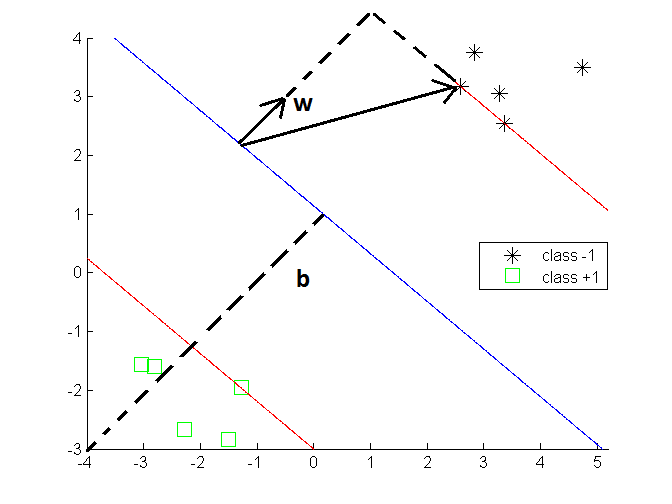
\includegraphics[width=0.7\linewidth]{images/SVM_interpretation2}
	\caption{Geometric representation of SVM.}
	\label{fig:SVM_interpretation}
\end{figure}

In the primal, the weight vector $\textbf{w} = [w_1, \ldots, w_p]^T$ contains as many elements as there are dimensions in the dataset, i.e., $\textbf{w} \in \mathbb{R}^p$. The magnitude of each element in $\textbf{w}$ denotes the importance of the corresponding variable for the classification problem. If the element of $\textbf{w}$ for some variable is 0, these variables are not used for the classification problem.

In order to visualize the above interpretation of the weight vector $\textbf{w}$, let us examine several hyperplanes $\textbf{w}^T\textbf{x}+b=0$ shown in Fig. \ref*{fig:Weight_interpretation} with $p=2$. Fig. \ref{fig:Weight_interpretation}(a) shows a hyperplane where elements of $\textbf{w}$ are the same for both variables $x_1$ and $x_2$. The interpretation is that both variables contribute equally for classification of objects into positive and negative. Fig. \ref{fig:Weight_interpretation}(b) shows a hyperplane where the element of $\textbf{w}$ for $x_1$ is 1, while that for $x_2$ is 0. This is interpreted as that $x_1$ is important but $x_2$ is not. An opposite example is shown in Fig. \ref{fig:Weight_interpretation}(c) where $x_2$ is considered to be important but $x_1$ is not. Finally, Fig. \ref{fig:Weight_interpretation}(d) provides a 3-dimensional example ($p=3$) where an element of $\textbf{w}$ for $x_3$ is 0 and all other elements are equal to 1. The interpretation is that $x_1$ and $x_2$ are important but $x_3$ is not.

\begin{figure}[h!]
	\centering
	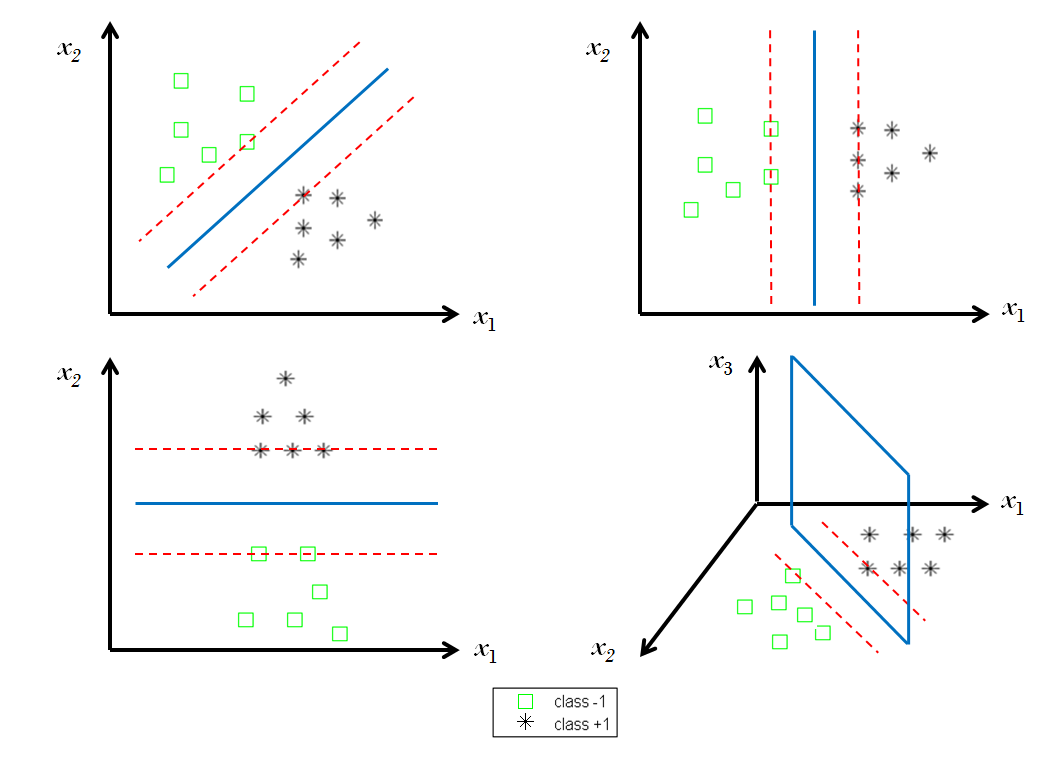
\includegraphics[width=1\linewidth]{Weight_interpretation3}
	\caption{Example of several {\sc svm}s and how to interpret the weight vector $\textbf{w}$}
	\label{fig:Weight_interpretation}
\end{figure}

Another way to interpret how much a variable contributes in the vector $\textbf{w}$ is to express the contribution in percentage: the ratio $\frac{w_j}{||\textbf{w}||_2} . 100$ defines the percentage of contribution for each variable $x_j$ in the {\sc svm} model. The interpretation is only valid if 
the variables $x_j$ of the time series are normalized before learning the {\sc svm} model, they evolves in the same range.



\noindent \textbf{Interpretation in the dual} \\
As a constrained optimization, the dual form satisfies the
Karush-Kuhn-Tucker ({\sc kkt}) conditions (Eqs. \ref{KKT1}, \ref{KKT2} and \ref{KKT3}). We recall Eq. \ref{KKT3}:
\begin{equation*}
	\alpha_i (y_i(\textbf{w}^T\textbf{x}_i+b)-1) = 0
\end{equation*}

From this, for every datapoint $\textbf{x}_i$, either $\alpha_i^* = 0$ or $y_i(\textbf{w}^T\textbf{x}_i+b) = 1$. Any datapoint with $\alpha_i^* = 0$ do not appear in the sum of the decision function $f$ in Eq. \ref{decisionDual} or \ref{decisionDualKernel}. Hence, they play no role for the classification decision of a new sample $\textbf{x}_j$. The others $\textbf{x}_i$ such that $\alpha_i^* > 0$ corresponds to the support vectors. Looking at the distribution of $\alpha_i^*$ allows also to have either a better understanding of the datasets, or either to detect outliers. The higher the coefficient $\alpha_i^*$ for a sample $\textbf{x}_i$ is, the more the sample $\textbf{x}_i$ impacts on the decision function $f$. However, an unusually high value of $\alpha_i^*$ among the samples can lead to two interpretations: either this point is a critical point to the decision, or this point is an outlier. In the soft margin formulation, by constraining $\alpha_i^*$ to be inferior to $C$ (Box constraints) the effect of outliers can be reduced and controlled. 

\subsubsection{Variants of {\sc svm}}
From the primal formulation of {\sc svm} (Eqs. \ref{eq:objectiveSVM} \& \ref{eq:constraintsSVM}), some works investigate the effect of modifications in the regularization and loss term \cite{Hsu2008}.

First, the two common regularizers are $||\textbf{w}||_1$ and $||\textbf{w}||_2$. The former is referred to as $L_1$-Regularizer while the latter is $L_2$-Regularizer. $L_1$-Regularizer is used to obtain sparser models than $L_2$-Regularizer, i.e., the vector $\textbf{w}$ will contain many elements $w_i$ that will equal to zero. Thus, it can be used for variable selection.

Secondly, the two common loss functions $\xi_i$ are $\max(1-y_i \textbf{w}^T \textbf{x}_i, 0)$ and $[\max(1-y_i \textbf{w}^T \textbf{x}_i, 0)]^2$. The former is referred to as $L_1$-Loss and the latter is $L_2$-Loss function. $L_2$-loss function will penalize more slack variables $\xi_i$ during training and would be more sensitive to outliers. Theorically, it should lead to less error in training and poorer generalization in most of the case \cite{Hsu2008}. In general, $L_1$-Loss is preferred.



\subsubsection{Extensions of {\sc svm}}
{\sc svm} has received many interests in recent years. Many extensions has been developed such as $\nu$-{\sc svm}, asymmetric soft margin {\sc svm} or multiclass {\sc svm} \cite{Kijsirikul2002,Crammer2001}. One interesting extension is the extension of Support Vector Machine to regression problems, also called Support Vector Regression ({\sc svr}). The objective is to find a linear regression model $f(\textbf{x})=\textbf{w}^T\textbf{x}+b$. To preserve the property of sparseness, the idea is to consider an $\epsilon$-insensitive error function. It gives zero error if the absolute difference between
the prediction $f(\textbf{x}_i)$ and the target $y_i$ is less than $\epsilon$ where $\epsilon > 0$ penalize samples that are outside of a $\epsilon$-tube as shown as in Fig. \ref{fig:SVR_tube}.

\begin{figure}[h!]
\centering
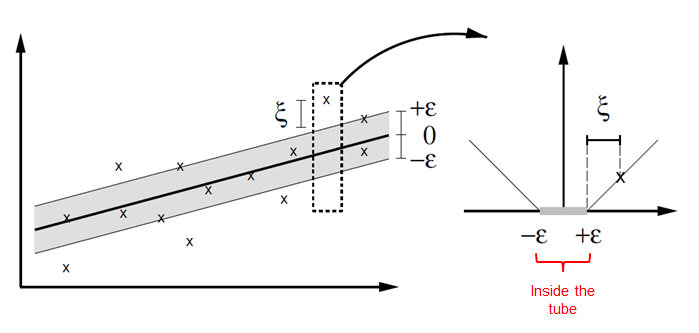
\includegraphics[width=0.8\linewidth]{images/SVR_tube}
\caption{Illustration of {\sc svm} regression (left), showing the regression curve with the $\epsilon$-insensitive "tube" (right). Samples $\textbf{x}_i$ above the $\epsilon$-tube have $\xi_1 > 0$ and $\xi_1 = 0$, points below the $\epsilon$-tube have $\xi_2 = 0$ and $\xi_2 > 0$, and points inside the $\epsilon$-tube have $\xi = 0$.}
\label{fig:SVR_tube}
\end{figure}

\noindent The $\epsilon$-insensitive error function $E_{\epsilon}$ is defined by:
\begin{equation}
E_{\epsilon} (f(\textbf{x}_i)-y_i) =
\left\lbrace
\begin{array}{lll}
0  								& \mbox{if} 		& |f(\textbf{x}_i)-y_i| < \epsilon\\
|f(\textbf{x}_i)-y_i|-\epsilon 	& \mbox{otherwise}  & 
\end{array}\right.
\end{equation}


\noindent The soft margin optimization problem in its primal form is formalized as:
	\begin{align}
		& \argmin_{\textbf{w},b}  \left( 
		\overbrace{\vphantom{\sum_{i=1}^n \xi_i}
			\frac{1}{2}||\textbf{w}||^2_2}^{Regularization}
		+ C \overbrace{\sum\limits_{i=1}^{n}(\xi_{i_1}+\xi_{i_2})}^{Loss}
		\right) 
		\label{eq:objectiveSVR}\\
		& \textbf{s.t. } \forall i=1 \ldots n: \nonumber\\
		& y_i-(\textbf{w}^T\textbf{x}_i+b) \geq \epsilon -\xi_{i_1} \\
		& (\textbf{w}^T\textbf{x}_i+b)-y_i \geq \epsilon -\xi_{i_2} \\
		&  \xi_{i_1} \geq 0 \\
		&  \xi_{i_2} \geq 0
	\end{align}

\noindent The slack variables are divided into 2 kind of slacks variables, one for samples above the decision function $f$ ($\xi_{i_1}$), and one for samples under the decision function $f$ ($\xi_{i_2}$). As for {\sc svm}, it is possible to have a dual formulation:
	\begin{align}
		& \argmax_{\boldsymbol{\alpha}} 
		\left( 
		\sum\limits_{i=1}^{n} y_i(\alpha_{i_1}-\alpha_{i_2})
		-\frac{1}{2} \sum\limits_{i=1}^{n} \sum\limits_{j=1}^{n} (\alpha_{i_1}-\alpha_{i_2})(\alpha_{j_1}-\alpha_{j_2}) (\textbf{x}_i.\textbf{x}_j)
		\right) \\ 
		& \textbf{s.t. } \forall i=1 \ldots n: \nonumber\\
		& \sum\limits_{i=1}^{n} \alpha_{i_1} = \sum\limits_{i=1}^{n} \alpha_{i_2} \\
		& 0 \leq \alpha_{i_1} \leq C \\
		& 0 \leq \alpha_{i_2} \leq C
	\end{align}
\noindent As in {\sc svm}, we obtain three possible regression functions for a new sample $\textbf{x}_j$, respectively in its primal, dual, and non-linear form:
\begin{align}
	& f(\textbf{x}_j) = \textbf{w}^T\textbf{x}_j+b \\ 
	& f(\textbf{x}_j) = \sum\limits_{i=1}^{n} (\alpha_{i_1}^*-\alpha_{i_2}^*)(\textbf{x}_i.\textbf{x}_j) + b \\	
	& f(\textbf{x}_j) = \sum\limits_{i=1}^{n} (\alpha_{i_1}^*-\alpha_{i_2}^*)K(\textbf{x}_i,\textbf{x}_j) + b
\end{align}	
More informations about the calculation development can be found in \cite{Bishop2006}.

\subsection{Other classification algorithms}
\todo[inline]{Partie non encore rédigée. A faire à la fin.}
\begin{itemize}
	\item Positionner les travaux par rapport aux autres méthodes d'apprentissage supervisé
	\item S'intéresser au Deep neural network (à la mode en ce moment)
	\item RVM, Decision Tree, 
	\item Ne pas trop développer
	\item Dans notre cas, on ne s'intéressera pas à ce type d'algorithmes (type deep learning) car il ne repose pas sur une notion de distance et les features qui sont trouvés ne sont pas interprétables
\end{itemize}



%----------------------------------------------------------------------------
\section{Conclusion of the chapter}
%\begin{itemize}
%	\item The concept of order of temporal data in not take into account (dynamic, frequence, etc.)
%	\item Introduction to next chapter: all of these algorithms (kNN, {\sc svm}, etc.) are based on a notion of distance or similarity between objects to compare/classify. Let consider now the object time series and let recall the concept of distance between time series
%\end{itemize}
\todo[inline]{A refaire complètement à la fin.}
This chapter reviews the different steps in a machine learning framework: data normalization, model selection and model evaluation. We focus on two machine learning algorithms used in our proposition: the $k$-Nearest Neighbors ($k$-NN) and the Support Vector Machine ({\sc svm}). In the following, we consider the $k$-NN as our classifier. The {\sc svm} will be used in our work for its large margin concept. 

Our objective being the learning of a metric that optimizes the performances of the $k$-NN classifier, we review in the next section some metrics proposed for time series as well as metric learning concept for static data.

%To make the classification or regression of time series, a commonly hypothesis is to consider time series as static data and then to apply classical machine learning algorithms, such as a $k$-Nearest Neighbors ($k$-NN) or a Support Vector Machine ({\sc svm}) approach. For that, the practitioner has to be careful on the design of his learning framework: data must be separated into a training and testing set, data have to be normalized depending on their distributions, cross-validation must be operated on the training set to learn the best fitting of the hyper-parameters and finally, performance metrics and statistical tests should be used to compare the performances of different classifiers.
%
%In the following, we consider the $k$-NN as our classifier. The {\sc svm} will be used in our work for its generalization properties thanks to the large margin concept. A key aspect in $k$-NN relies on the comparison of time series through metrics. Assuming that time series can be reduced to flat data may be too restrictive. Under such hypothesis and using a standard Euclidean distance, time series are only compared on their amplitude at the same time. However, time series are more complex. They may exhibit similar behavior or share similar frequential spectrum. Thus, there is a need to consider time series as an ordered object and to define adapted metrics for time series.


%%% Local Variables: 
%%% mode: latex
%%% TeX-master: "../roque-phdthesis"
%%% End: 

\chapter{Time series metrics and metric learning}
\label{sec:Chapter_metrics}
\minitoc

% \noindent Chapeau introductif
%\begin{itemize}
%	\item Rappel : notion de similaire : dans le cadre de la classification, on a un comportement « similaire » pour une même classe. La notion de « similaire » est lié à une notion de distance ou (dis)similarité. 
%	\item Donner les hypothèses de travail : 
%	\begin{itemize}
%		\item Considérons la série temporelle comme étant un objet ordonné.
%		\item les séries temporelles sont de même taille
%		\item les séries temporelles ont la même période d'échantillonnage
%		\item les séries temporelles peuvent être comparés sur l'ensemble des valeurs, sur une partie des valeurs, sur un ensemble de fenêtre (fréquences, etc.)
%	\end{itemize}
%	\item On va définir dans la suite la notion de métrique, d'alignement, de localité pour des séries temporelles.
%	\item Mettre un graphique (dit GRAPHIQUE GENERAL) qui prend 5 séries temporelles que l'on va utiliser pour la suite : proche en valeur, proche en forme, proche en fréquence, proche en valeur avec un délai, proche en forme avec un délai
%\end{itemize}

\fbox{  \parbox{0.9\textwidth}{
		In this chapter, we first present the definition of time series. Then, we recall the general properties of a metric and introduce some metrics proposed for time series. In particular, we focus on amplitude-based, behavior-based and  frequential-based metrics. As real time series are subject to varying size and delays, we recall the concept of alignment and dynamic programming. Then, we present some proposed combined metrics for time series. Finally, we review the concept of metric learning.
		% In this chapter, we review different metrics for time series. In classification problems, time series are expected to be similar if they belong to the same class. The concept of similarity among time series is directly linked to the concept of metrics. \\
		
		% In the following, we consider time series as an object. They may be compared either on all their observations $x_{it}$, a part of them or in a window. We first recall the properties of a metric. Then, we review three types of metrics (amplitude-based, behavior-based, frequential-based) and kernels adapted to time series. As real time series are subjected to varying delays, we recall the concept of alignment and dynamic programming. We show how these metrics can be used to define either metrics that can capture local characteristics of time series, or metrics that combine multiple modalities. Finally, as $k$-NN performances is directly impacted by the choice of the metric, we review some insights on Metric Learning investigated in the case of static data.
	}  }


\section{Definition of a time series}
% We call time series, a collection of numerical observations made sequentially in the time. It is characterized by a finite number of realized observations made at discrete instants of time $t=1,...,T$. 
Time series are data that 
% may occur in physical sciences (meteorology, marine science, geophysics), marketing or process control \cite{Chatfield2004}. Time series 
can be frequently found in various emerging applications such as sensor networks, smart buildings, social media networks or Internet of Things (IoT) \cite{Najmeddine2012,Nguyen2012,Yin2008}. They are involved in many learning problems such as recognizing a human movement in a video, detecting a particular operating mode, etc. \todo{Ajouter virtual sensors?} \cite{PANAGIOTAKIS2008,Ramasso2008}. In \textbf{clustering} problems, one would like to organize similar time series together into homogeneous groups. In \textbf{classification} problems, the aim is to assign time series to one of several predefined categories (e.g., different types of defaults in a machine). In \textbf{regression} problems, the objective is to predict a continuous value from observed time series (e.g., forecasting the measurement of a power meter from pressure and temperature sensors). Due to their temporal and structured nature, time series constitute complex data to be analyzed by classic machine learning approaches.

For physical systems, a time series of duration $T$ can be seen as a signal, sampled at a frequency $f_e$, in a temporal window $[0;T]$. From a mathematical perspective, a time series of length $Q$ is a collection of a finite number of observations made sequentially at discrete time instants $t=1,...,Q$. Note that $Q=Tf_e$. 

Let $\textbf{x}_i=(x_{i1}, x_{i2}, ..., x_{iQ})$ be a univariate time series of length $Q$. Each observation $x_{it}$ is bounded (i.e., the infinity is not a valid value: $x_{it} \neq \pm \infty$). The time series $\textbf{x}_i$ is said to be univariate if the collection of observations $x_{it}$ ($t=1,...,Q$) comes from the observation of one variable (i.e., the temperature measured by one sensor). When simultaneous observation of $p$ variables (several sensors such as the temperature, the pressure, etc.) are made at the same time, the time series is said to be multivariate. From this, one possible representation would be: 
\begin{equation*}
	\textbf{x}_i=(x_{i1,1}, ..., x_{i1,p},x_{i2,2}, ..., x_{i2,2}, ..., x_{iQ,p})
\end{equation*}
\noindent where $\textbf{x}_{it,j}$ is the observation of the time series $\textbf{x}_{i}$ at the time instant $t$ along the variable $x_j$. An other possible representation could consider a multivariate time series $\textbf{x}_i$ as the union of multiple univariate time series. In this case: 
\begin{equation*}
	\textbf{x}_i=(\textbf{x}_{i,1}, ...., \textbf{x}_{i,p})=(x_{i1,1}, ..., x_{iQ,1},x_{i1,2}, ..., x_{i1,p}, ..., x_{iQ,p})
\end{equation*}
where $\textbf{x}_{i,j} = (\textbf{x}_{i1,j}, \ldots, \textbf{x}_{iQ,j})$. For simplification purpose, we only consider univariate time series in the following. 

\missingfigure{Ajouter une figure pour les 2 représentations des ST multivariées}

Some authors propose to extract representative features from time series. Fig.~\ref{fig:time_series_example} illustrates a model for time series proposed by Chatfield in \cite{Chatfield2004}. It states that a time series can be decomposed into 3 components: a trend, a cycle (periodic component) and a residual (irregular variations). 

\begin{figure}[h!]
	\centering
	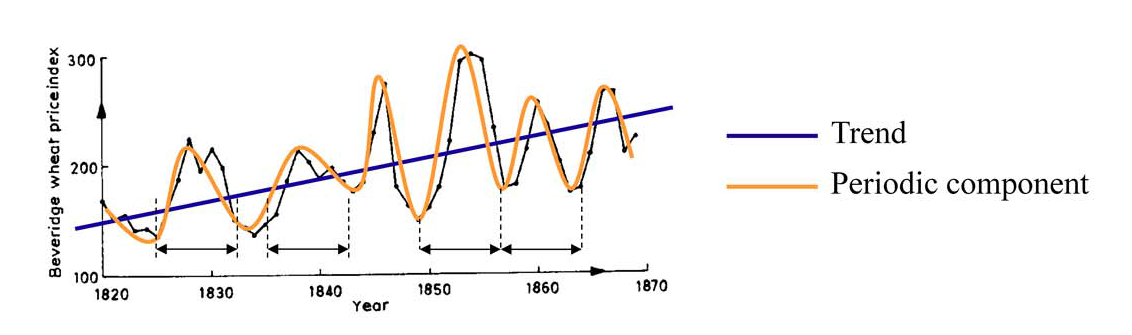
\includegraphics[width=1\linewidth]{images/time_series_example}
	\caption{The Beveridge wheat price index is the average in nearly 50 places in various countries measured in successive years from 1500 to 1869. \protect\footnotemark}
	\label{fig:time_series_example}
\end{figure}
\footnotetext{This time series can be downloaded from \url{http://www.york.ac.uk/depts/maths/data/ts/ts04.dat}}

\noindent According to Chatfield, most time series exhibit either or both a long term change in the mean (trend) and a periodic (cyclic) component. The trend can be linear, quadratic, etc. The cyclic component is a variation at a fixed period of time (seasonality) such as for example the seasonal variation of temperature. In practice, the 3 features (trend, cycle, residuals) are rarely sufficient for the classification or regression of real time series. 
% In our work, we propose to focus on the raw time series and do not try to extract global features from the time series.

Other authors made the hypothesis of time independency between the observations $x_{it}$. They consider time series as a static vector data and use classic machine learning algorithms \cite{Liang2012,Cao2001,Hu2013,Hwang2012}. Our work focuses on classification and regression problems, and on time series comparison through metrics.


% Nous désignons par données temporelles des données numériques évoluant dans le temps, dites communément séries temporelles, ou des suites chronologiques de données symboliques dites séquences temporelles. Plus généralement, on désigne par données de séquences toute collection de données ordonnées selon un critère qui peut être sémantique, biologique, temporel ou autre ; c’est le cas, par exemple, des séquences de mots dans un texte ; on parle alors d’ordre syntaxique, de séquences d’acides aminés composant une chaîne d’ADN ou de peptides constituant une protéine.




%-----------------------------------------------------------------------------
\section{Properties and representation of a metric}
\label{sec:property_metric}
%\begin{itemize}
%	\item Rappeler les propriétés d'une mesure de distance (positivité, symétrique, distinguabilité, inégalité triangulaire)
%	\item Donner les différences entre métriques, distance, dissimilarités, similarités, pseudo-métrique, etc.
%	\item Dans la suite du travail, on va tout assimiler au mot métrique pour une meilleure simplicité
%\end{itemize}

A mapping $D:\mathbb{R}^p \times \mathbb{R}^p \rightarrow \mathbb{R}^+$ over a vector space $\mathbb{R}^p$ is called a metric or a distance if for all vectors $\forall \textbf{x}_i, \textbf{x}_j, \textbf{x}_l \in \mathbb{R}^p$, it satisfies the properties:
\mycomment[CTD]{je préfère garder l'espace pour + de visibilité}\begin{enumerate}
	\item {\makebox[6cm]{$D(\textbf{x}_i, \textbf{x}_j) \geq 0$\hfill} (positivity)}
	\item {\makebox[6cm]{$D(\textbf{x}_i, \textbf{x}_j) = D(\textbf{x}_j, \textbf{x}_i)$\hfill} (symmetry)}	
	\item {\makebox[6cm]{$D(\textbf{x}_i, \textbf{x}_j) = 0 \Leftrightarrow  \textbf{x}_i=\textbf{x}_j$\hfill} (distinguishability)}
	\item {\makebox[6cm]{$D(\textbf{x}_i, \textbf{x}_j) + D(\textbf{x}_j, \textbf{x}_l) \geq D(\textbf{x}_i, \textbf{x}_l)$\hfill} (triangular inequality)}
\end{enumerate}
A mapping $D$ that satisfies at least properties 1, 2, 3 is called a dissimilarity, and the one that satisfies at least properties 1, 2, 4 a pseudo-metric. A metric, a dissimilarity and a pseudo metric can be both interpretated as a measure of how "different" two samples are. Note that theu can be used for comparisons of several samples: if a time series $\textbf{x}_i$ is expected to be closer to $\textbf{x}_j$ than to $\textbf{x}_l$, then $D(\textbf{x}_i,\textbf{x}_j) \leq D(\textbf{x}_i,\textbf{x}_l)$. On the contrary, the mapping is called a similarity $S$ when the sample $\textbf{x}_i$ is expected to be closer to $\textbf{x}_j$ than to $\textbf{x}_l$ and then $S(\textbf{x}_i,\textbf{x}_j) \geq S(\textbf{x}_i,\textbf{x}_l)$. To simplify the discussion in the following, we refer to pseudo-metric and dissimilarity as metrics, pointing out the distinction only when necessary.

Metric can be represented in two ways. First, data points (samples $\textbf{x}_i$) can be fixed and the distance sphere is shown. Secondly, the distance sphere can be fixed and the data points and the axis are moving.

\missingfigure{représentation métrique}



%-----------------------------------------------------------------------------
\section{Unimodal metrics for time series}
Defining and evaluating metrics for time series has become an active area of research for a wide variety of problems in machine learning \cite{Ding2008, Najmeddine2012}. In the following, we suppose that time series have the same duration $T$ and have been regularly sampled at the frequency $f_e$. Therefore, they have the same length $Q=Tf_e$. Let $\textbf{x}_i=(x_{i1}, x_{i2}, ..., x_{iQ})$ and $\textbf{x}_j=(x_{i1}, x_{i2}, ..., x_{iQ})$ be two univariate time series of length $Q$. 

A large number of distance measures have been proposed in the literature \cite{Montero2014}. Contrary to static data, time series may exibit modalities and specificities due to their temporal nature (e.g., value, shape, frequency, delay, temporal locality). In this section, we review 3 categories of time series metrics used in our work: amplitude-based, frequential-based and behavior-based.



%To illustrate the effect of different metrics, we will consider some toy examples of time series, illustrated in Fig. \ref{fig:ExampleTimeSeriesMetrics}. The objective is to determine which time series is closer to $\textbf{x}_1$. Based on the amplitude of the signals, it is straightforward that $\textbf{x}_2$ is the closest to $\textbf{x}_3$. However, if we consider the shape of the signal, $\textbf{x}_1$ is the closest to $\textbf{x}_3$. $\textbf{x}_1$ and $\textbf{x}_4$ can be considered also as the closest in value if we delete the effect of delays between the two time series. Finally, it seems that $\textbf{x}_1$ and $\textbf{x}_5$ share the same frequential components.
%
%\begin{figure}[h!]
%\centering
%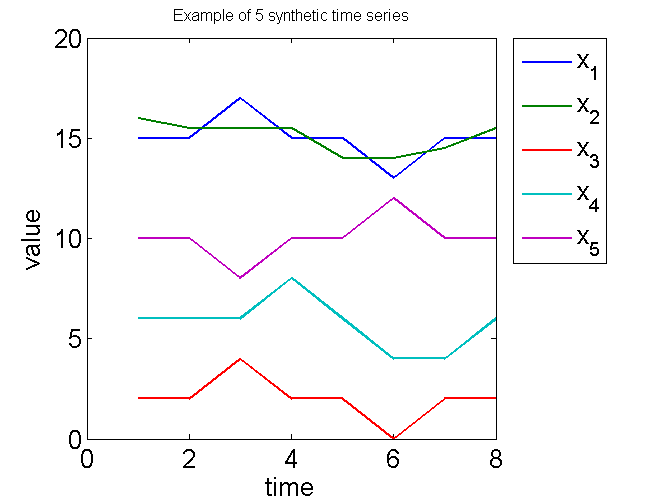
\includegraphics[width=0.6\linewidth]{images/ExampleTimeSeriesMetrics2}
%\caption{An example of 4 time series that can be compared on different distinct modalities. The objective is to determine which time series is closer to $\textbf{x}_3$.}
%\label{fig:ExampleTimeSeriesMetrics}
%\end{figure}
%\todo[  size=\tiny, color=green]{Reparler avec Michèle et Sylvain de la figure. J'aimerai pouvoir trouver 5 séries temporelles qui couvrirait ces cas.}




\subsection{Amplitude-based metrics}
\label{sec:TSmetrics}
%\begin{itemize}
%	\item Distance classiquement utilisée dans la littérature 
%	\item Distance de Minkowski (norm Lp)
%	\item Distance de Mahalanobis (norm pondéré)
%	\item $D_E$	qui est une forme particulière de Minkowski
%	\item Prendre le GRAPHIQUE GENERAL et faire le calcul des distances entre les courbes et montrer que pour 2 courbes qui ont des "amplitudes proches", on obtient une valeur de distance faible. 
%\end{itemize}

The most usual comparison measures are amplitude-based metrics, where time series are compared in the temporal domain on their amplitudes regardless of their behaviors or frequential characteristics. Among these metrics, there are the commonly used Euclidean distance that compares elements observed at the same time \cite{Ding2008}: 
\begin{equation}	
	d_E(\textbf{x}_i,\textbf{x}_j) = \sqrt{\sum\limits_{t=1}^{Q} (x_{it}-x_{jt})^2}
\label{eq:A}
\end{equation}
Note that the Euclidean distance is a particular case of the Minkowski $L_p$ norm ($p=2$). An other amplitude-based metric is the Mahalanobis distance \cite{Prekopcsak2012}, defined as a dissimilarity measure weighted by a matrix \textbf{M}:
\begin{equation}	
	d_M(\textbf{x}_i,\textbf{x}_j) = (\textbf{x}_i-\textbf{x}_j)^T\textbf{M}^{-1}(\textbf{x}_i-\textbf{x}_j)
	\label{eq:dM}
\end{equation}

If the covariance matrix $\textbf{M}$ is the identity matrix, the Mahalanobis distance is equal to the Euclidean distance. If the covariance matrix $\textbf{M}$ is diagonal, then the resulting distance measure is called a normalized Euclidean distance:
\begin{equation}	
d_M(\textbf{x}_i,\textbf{x}_j) = \sqrt{\sum\limits_{t=1}^{Q}\frac{(x_{it}-x_{jt})^2}{m_t}}
\label{eq:dM2}
\end{equation}
\noindent where $m_t$ is the variance of the $x_{it}$ and $x_{jt}$ over the sample set. Note that this is equivalent to normalize each feature: $x'_{il} = x_{il}/\sqrt{m_l}$ and use the Euclidean distance on the normalized features.
%\noindent In particular, when $\textbf{M}$ is a diagonal matrix, the previous formula becomes: 
%%\textbf{M} &= 	
%%\begin{pmatrix}
%%	M_1 & 0 & ... & 0 \\
%%	0 & M_2 & ... & 0 \\
%%	... \\
%%	0 & ... & & M_m 
%%\end{pmatrix} \\
%\begin{align}
%M &= 
%	\left(
%	\begin{array}{ccccc}
%	M_1\\
%	& ... & & \text{\huge0}\\
%	& & M_t & &\\
%	& \text{\huge0} & & ... \\
%	& & & & M_T
%	\end{array}
%	\right)	\\
%d_M(\textbf{x}_i,\textbf{x}_j) & = \sqrt{\sum\limits_{t=1}^{T} M_t(x_{it}-x_{jt})^2}
%\label{eq:dM2}
%\end{align}
%In practice, the $M_t$ coefficients are often set as the variance of the value on the corresponding dimension. \mycomment[MR]{Plus les données sont imprécises, moins elle est importante}Intuitively, each dimension difference ($x_{it}-x_{jt}$) is weighed by a factor $M_t$. It is also known as the weighted Euclidean distance \cite{McNames2002}. 
In the following of the work, we consider the standard Euclidean distance $d_E$ as the amplitude-based distance $d_A$.

\begin{figure}[h!]
\centering
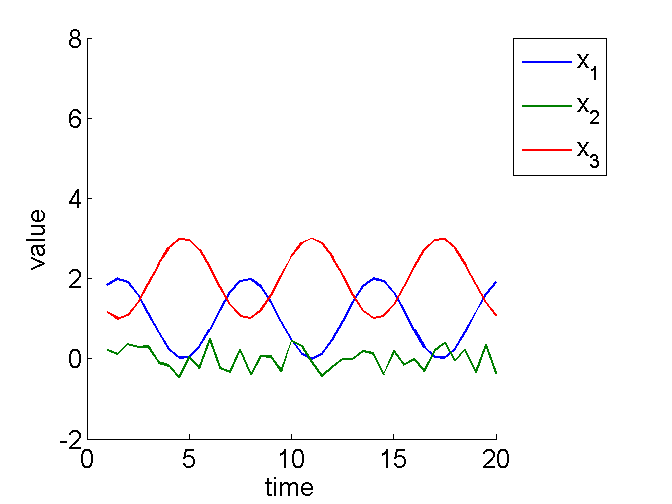
\includegraphics[width=0.6\linewidth]{images/ExampleTimeSeriesMetrics3}
\caption{3 toy time series. Time series in blue and red are two sinusoïdal signals. Time series in green is a random signal.}
\label{fig:ExampleTimeSeriesMetrics3}
\end{figure}

In the example of Fig. \ref{fig:ExampleTimeSeriesMetrics3}, the aim is \mycomment[SMA]{reformulation à revoir: let's try to} to determine which time series ($\textbf{x}_2$ or $\textbf{x}_3$) is the closest to $\textbf{x}_1$. The amplitude-based distance $d_A$ states that $\textbf{x}_2$ is closer to $\textbf{x}_1$ than $\textbf{x}_3$ since $d_A(\textbf{x}_1,\textbf{x}_2) = 7.8816 < d_A(\textbf{x}_1,\textbf{x}_3)= 31.2250$.



\subsection{Frequential-based metrics}
%\begin{itemize}
%	\item Dans le cadre du traitement de signal, les gens utilisent des représentations fréquentielles (Fourier, etc.)
%	\item Rappeler la transformée de Fourier (TF) + spectre (module de la TF)
%	\item On peut définir une distance dans la représentation de Fourier.
%	\item Prendre le GRAPHIQUE GENERAL et faire le calcul des distances entre les courbes et montrer que pour 2 courbes qui ont des "spectres proches", on obtient une valeur de distance faible. 
%\end{itemize}
The second category, commonly used in signal processing, relies on comparing time series based on their frequential properties (e.g. Fourier Transform, Wavelet, Mel-Frequency Cepstral Coefficients \cite{Sahidullah2012,Torrence1998,Brigham1967}). In our work, we limit the frequential comparison to Discrete Fourier Transform \cite{Lhermitte2011a}, but other frequential properties can be used as well. Thus, for time series comparison, first the time series $\textbf{x}_i$ are transformed into their Fourier representation $\tilde{\textbf{x}}_i=[\tilde{x}_{i1}, ...,  \tilde{x}_{iF}]$, with $\tilde{x}_{if}$ the complex component at frequential index $f$. The Euclidean distance is then used  between their respective complex number modules $|\tilde{x}_{if}|$:
\begin{equation}
d_{F}(\textbf{x}_i,\textbf{x}_j) = \sqrt{\sum_{f=1}^{F} 
	(|\tilde{x}_{if}|-|\tilde{x}_{jf}|)^2}
\label{eq:F}
\end{equation}

In the example of Fig. \ref{fig:ExampleTimeSeriesMetrics3}, the frequential-based distance $d_F$ states that the time series $\textbf{x}_3$ is closer to $\textbf{x}_1$ than $\textbf{x}_2$ since $d_F(\textbf{x}_1,\textbf{x}_3) = 0.8519 < d_F(\textbf{x}_1,\textbf{x}_2) = 0.9250$. This can be illustrated in the Frequency domain (Fig. \ref{fig:ExampleTimeSeriesMetrics3_freq})

%\begin{figure}[h!]
%	\centering
%	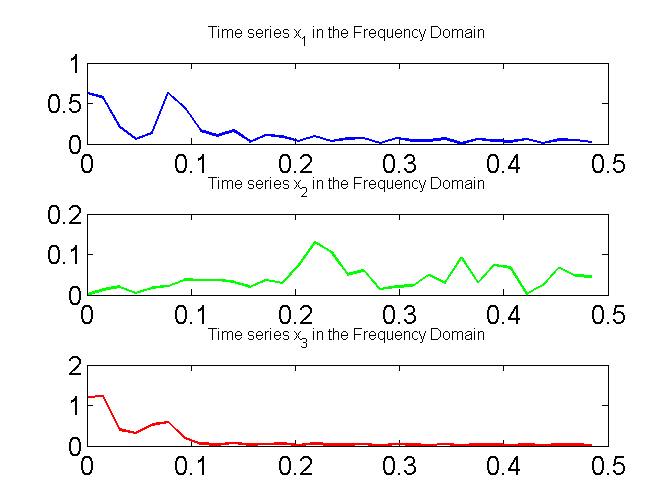
\includegraphics[width=0.7\linewidth]{images/ExampleTimeSeriesMetrics3_freq}
%	\caption{Frequency representation of the signal from Fig. \ref{fig:ExampleTimeSeriesMetrics3}. The spectrum (based on the comparison between frequencies) shows more similarities between signal $\textbf{x}_1$ (blue) and $\textbf{x}_3$ (red) than in the temporal domain (based on the comparison between temporal time t).}
%	\label{fig:ExampleTimeSeriesMetrics3_freq}
%\end{figure}
\missingfigure{Ajouter la représentation fréquentielle des signaux}


\subsection{Behavior-based metrics}
%\begin{itemize}
%	\item Intuition : expliquer ce que signifie "2 séries temporelles sont proches en forme".
%	\item Dans la littérature classique, on trouve la corrélation de Pearson
%	\item Récemment, Douzal \& al. propose une généralisation: cort
%	\item Transformer la cort en mesure de dissimilarité
%	\item Prendre le GRAPHIQUE GENERAL et faire le calcul des distances entre les courbes et montrer que pour 2 courbes qui ont des "formes proches", on obtient une valeur de distance faible. 
%\end{itemize}

The third category of metrics aims to compare time series based on their shape or behavior despite the range of their amplitudes. By time series of similar behavior, it is generally intended that for all temporal window $[t,t']$, they increase or decrease simultaneously with the same growth rate. On the contrary, they are said of opposite behavior if for all $[t,t']$, if one time series increases, the other one decreases and (vise-versa) with the same growth rate in absolute value. Finally, time series are considered of different behaviors if they are not similar, nor opposite. Many applications refer to the Pearson correlation~\cite{Abraham2010a,Benesty2009} for behavior comparison. A generalization of the Pearson correlation is introduced in~\cite{AhlameDouzal-Chouakria2011}: 
\begin{equation}	
	cort_r(\textbf{x}_i,\textbf{x}_j) = 
	\frac{
		\sum\limits_{t,t'=1}^Q 
		{
			(x_{it}-x_{it'})
			(x_{jt}-x_{jt'})
		}
	}
	{
		\sqrt{
			\sum\limits_{t,t'=1}^Q  
			{(x_{it}-x_{it'})^2}
		} 
		\sqrt{
			\sum\limits_{t,t'=1}^Q  
			{(x_{jt}-x_{jt'})^2}
		} 	 
	}
\label{eq:corTr}
\end{equation}

\noindent where $|t-t'| \leq r$, $r \in [1,..., Q-1]$. The parameter $r$ can be tuned or fixed a priori. It measures the importance of noise in data. For non-noisy data, low orders $r$ is generally sufficient. For noisy data, the practitioner can either use de-noising data technics (Kalman or Wiener filtering \cite{Kalman1960,WienerN1942}), or fix a high order $r$.

The temporal correlation $cort$ computes the sum of growth rate between $\textbf{x}_i$ and $\textbf{x}_j$ between all pairs of values observed at $[t ,t']$ for $t' \leq t+r$ ($r$-order differences). The value $cort_r(\textbf{x}_i,\textbf{x}_j) = +1$ means that $\textbf{x}_i$ and $\textbf{x}_j$  have similar behavior, i.e, there exists some constant $c$ such that $\textbf{x}_i = \textbf{x}_j+c$. The value $cort_r(\textbf{x}_i,\textbf{x}_j) = -1$ means that $\textbf{x}_i$ and $\textbf{x}_j$ have opposite behavior, i.e, there exists some constant $c$ such that $\textbf{x}_i = -\textbf{x}_j+c$. Finally, $cort_r(\textbf{x}_i,\textbf{x}_j) = 0$ expresses that their growth rates are stochastically linearly independent (different behaviors). 

% When $r=1$, Eq.~\eqref{eq:corTr} leads to the temporal correlation coefficient $cort$ \cite{AhlameDouzal-Chouakria2011}. 
When $r=Q-1$, it leads to the Pearson correlation. As $cort_r$ is a similarity measure, it can be transformed into a dissimilarity measure:
\begin{equation}
	d_B(\textbf{x}_i,\textbf{x}_j) = \frac{1 - cort_r(\textbf{x}_i,\textbf{x}_j)}{2}
	\label{eq:B}
\end{equation}

\begin{figure}[h!]
	\centering
	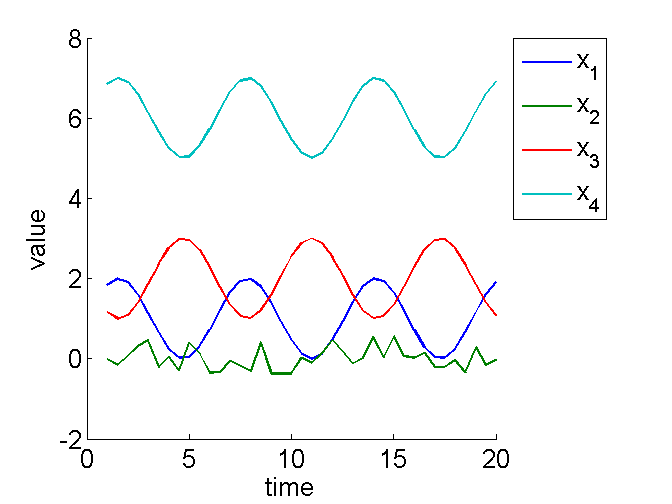
\includegraphics[width=0.7\linewidth]{images/ExampleTimeSeriesMetrics4}
	\caption{The signal from Fig. \ref{fig:ExampleTimeSeriesMetrics3} and a signal $\textbf{x}_4$ which is signal $\textbf{x}_1$ and an added translation. Based on behavior comparison, $\textbf{x}_4$ is the closest to $\textbf{x}_1$.}
	\label{fig:ExampleTimeSeriesMetrics4}
\end{figure}

\noindent Considering Fig. \ref{fig:ExampleTimeSeriesMetrics4}, we obtain:
\begin{align*}
d_B(\textbf{x}_1,\textbf{x}_2) &= 0.477 \\  
d_B(\textbf{x}_1,\textbf{x}_3) &= 1 \\  
d_B(\textbf{x}_1,\textbf{x}_4) &= 0 \\ 
\label{key}
\end{align*}  

\subsection{Other metrics and Kernels for time series}
\todo[inline]{A faire à la fin, pas urgent}
\begin{itemize}
	\item Il existe dans la littérature de nombreuses autres métriques pour les séries temporelles (laisser la porte ouverte).
	\item Certaines métriques sont utilisées dans le domaine temporelle
	\item D'autres métriques sont utilisés dans d'autres représentations (Wavelet, etc.)
	\item Certaines combinent la représentation temporelles et fréquentielles (Représentation spectrogramme en temps-fréquence)
	\item Se baser sur l'article "TSclust : An R Package for Time Series Clustering".
	\item Fermer le cadre : dans la suite de notre travail, on ne va pas les utiliser mais elles pourront être intégrées dans le framework qui suivra au chapitre suivant
\end{itemize}


%-----------------------------------------------------------------------------
\section{Time series alignment and dynamic programming approach}
%\begin{itemize}
%	\item Les données réelles peuvent présenter des délais, des changements de dynamique de l'échelle de temps : extension, compression (dans la limite du raisonnable).
%	\item Il existe des techniques qui permettent de ré-aligner les séries temporelles comme la DTW
%	\item Définir la notion d'alignement
%	\item Présenter la DTW (+ algorithme)
%	\item Présenter les variantes de la DTW
%	\item Dans la suite du travail, on suppose que les séries temporelles sont ré-alignées.
%	\item Prendre le GRAPHIQUE GENERAL et faire le calcul des distances entre les courbes et montrer que pour 2 courbes qui ont des "valeurs proches" mais décalés, on obtient une valeur de distance faible. (prendre DTW standard avec une fonction de coût $D_E$ par exemple)
%\end{itemize}

\mycomment[SMA]{formulation totale à revoir} In some applications, time series needs to be compared at different time $t$ (i.e. energy data \cite{Najmeddine2012}) whereas in others, comparing time series on the same time $t$ is essential (i.e. gene expression \cite{Chouakria2007}). When time series are asynchronous (i.e. varying delays or dynamic changes), they must be aligned before any analysis process. The asynchronous effects can be of various natures: time shifting (phase shift in signal processing), time compression or time dilatation. For example, in the case of voice recognition (Fig. \ref{fig:Voice_Example}), it is straightforward that a same sentence said by two different speakers will produce different time series: one speaker may speak faster than the other; one speaker may take more time on some vowels, etc.

\begin{figure}[h!]
\centering
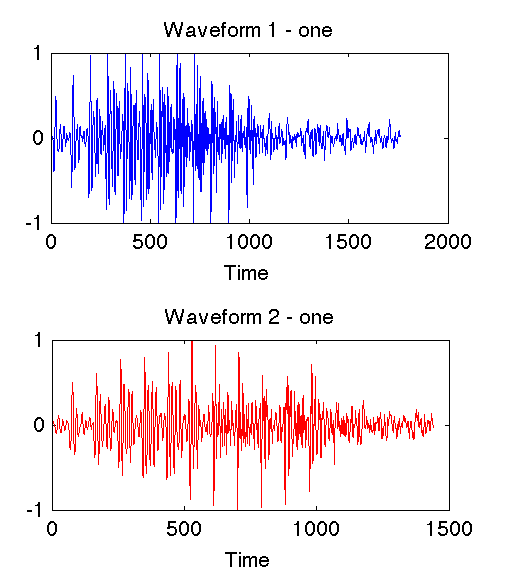
\includegraphics[width=0.5\linewidth]{images/Voice_Example}
\caption{Example of a same sentence said by two different speakers. Time series are shifted, compressed and dilatated in the time.}
\label{fig:Voice_Example}
\end{figure}
\mycomment[MR]{Modifier figure. enlever 'one' et mettre la même échelle temporelle}
To cope with delays and dynamic changes, dynamic programming approach has been introduced \cite{Berndt1994a}. An alignment $\boldsymbol{\pi}$ of length $|\boldsymbol{\pi}_{ij}|=m$ between two time series $\textbf{x}_i$ and $\textbf{x}_j$ of length $Q$ is defined as the set of $m$ ($Q \leq m \leq 2Q-1$) couples of aligned elements of $\textbf{x}_i$ to $m$ elements of $\textbf{x}_j$:
\begin{equation}
\boldsymbol{\pi}_{ij} = 
\left(  
(\pi_i(1),\pi_j(1)), 
(\pi_i(2),\pi_j(2)), 
\ldots,
(\pi_i(m),\pi_j(m))
\right) 
\end{equation}
\mycomment[AD]{Ahlame pas fan des notations}
\noindent where the applications $\pi_i$ and $\pi_j$ defined from $\{1, ..., m\}$ to $\{1, ..., Q\}$ obey the following boundary monotonicity conditions: 
\begin{align}
& 1 = \pi_i(1) \leq \pi_i(2) \leq ... \leq \pi_i(m) = Q \\
& 1 = \pi_j(1) \leq \pi_j(2) \leq ... \leq \pi_j(m) = Q 
\end{align}
$\forall l \in \{1, ..., m\}$, 
\begin{align}
& \pi_i(l+1) \leq \pi_i(l)+1 \\
\text{  and  \qquad} & \pi_j(l+1) \leq \pi_j(l)+1 \\
\text{  and  \qquad} & ( \pi_i(l+1)-\pi_i(l) ) - ( \pi_j(l+1)-\pi_j(l)) \geq 1 . 
\end{align}
In the following, we denote $\boldsymbol{\pi}=\boldsymbol{\pi}_{ij}$ to simplify the notation. Intuitively, an alignment $\boldsymbol{\pi}$ defines a way to associate elements of two time series. Alignments can be described by paths in the $Q \times Q$ grid that crosses the elements of $\textbf{x}_i$ and $\textbf{x}_j$ (Fig. \ref{fig:DTWgrid}). We denote $\boldsymbol{\pi}$ a valid alignment and $A$, the set of all possible alignments between $\textbf{x}_i$ and $\textbf{x}_j$ ($\boldsymbol{\pi} \in A$). To find the best alignment $\boldsymbol{\pi}^*$ between two time series $\textbf{x}_i$ and $\textbf{x}_j$, the Dynamic Time Warping (\textsc{dtw}) algorithm has been proposed \cite{Keogh2004,Salvador}.

\textsc{dtw} requires to choose a cost function $\varphi$ to be optimised, such as a dissimilarity function ($d_A, d_B$, $d_F$, etc.). Classical \textsc{dtw} uses the Euclidean distance $d_A$ (Eq. \ref{eq:A}) as the cost function~\cite{Berndt1994a}. The warp path $\boldsymbol{\pi}$ is optimized for the chosen cost function $\varphi$:
\begin{equation}
\boldsymbol{\pi}^* = \argmin_{\boldsymbol{\pi} \in A} \frac{1}{|\boldsymbol{\pi}|}
\sum_{(t,t') \in \boldsymbol{\pi}} \varphi(x_{it}, x_{jt'})
\label{eq:DTW}
\end{equation}

\noindent When the cost function $\varphi$ is a similarity measure, the optimization involves maximization instead of minimization. When other constraints are applied on $\boldsymbol{\pi}$, Eq. \eqref{eq:DTW} leads to other variants of \textsc{dtw} (Sakoe-Shiba \cite{Sakoe1978a}, Itakura parallelogram \cite{Rabiner1993}). Finally, the warped signals $\textbf{x}_{i,\boldsymbol{\pi}^*}$ and $\textbf{x}_{j,\boldsymbol{\pi}^*}$ are defined as:
\begin{align}
\textbf{x}_{i,\boldsymbol{\pi}^*} 
&= (x_{i\pi_i(1)}, ..., 
x_{i\pi_i(m)}) 			\\	
\textbf{x}_{j,\boldsymbol{\pi}^*} 
&= (x_{j\pi_j(1)}, ..., 
x_{j\pi_j(m)}) 	
\end{align}

\begin{figure}[h!]
	\centering
	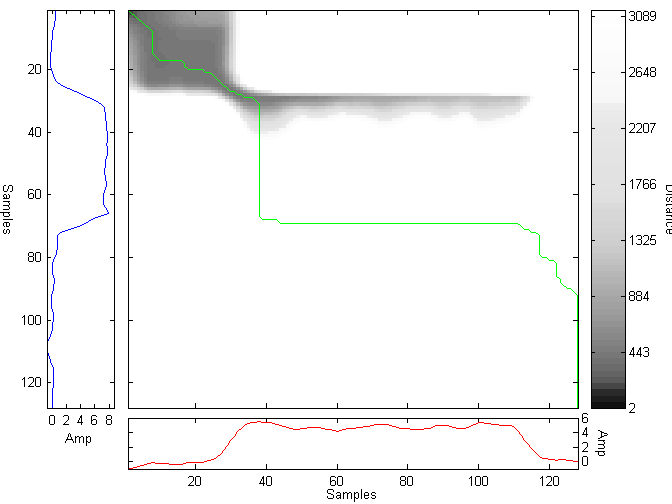
\includegraphics[width=0.5\linewidth]{images/DTWgrid2}
	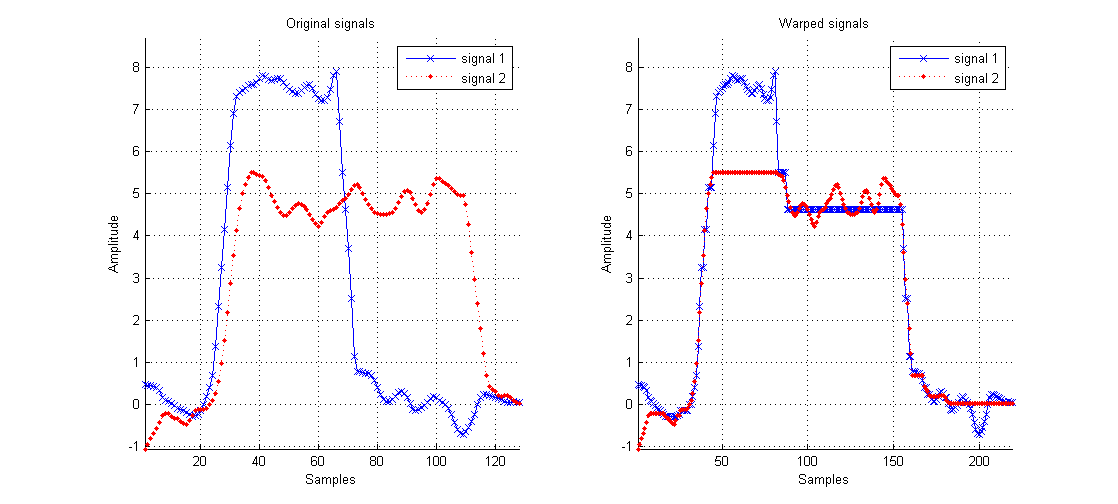
\includegraphics[width=0.9\linewidth]{images/DTWwarpedSignals}
	\caption{Example of {\sc dtw} grid between 2 time series $\textbf{x}_{i}$ and $\textbf{x}_{j}$ (top) and the signals before and after warping (bottom). On the {\sc dtw} grid, the two signals can be represented on the left and bottom of the grid. The optimal path $\boldsymbol{\pi}^*$ is represented in green line and shows how to associate elements of $\textbf{x}_{i}$ to element of $\textbf{x}_{j}$. Background show in grey scale the value of the considered metric (amplitude-based distance $d_A$ in classical {\sc dtw})}
	\label{fig:DTWgrid}
\end{figure}


The previous metric (amplitude-based $d_A$, behavior-based $d_B$) can be then computed on the warped signals $\textbf{x}_{i,\boldsymbol{\pi}^*}$ and $\textbf{x}_{j,\boldsymbol{\pi}^*}$. In the following, we suppose that the best alignment $\boldsymbol{\pi}^*$ is found. For simplification purpose, we refer $\textbf{x}_{i,\boldsymbol{\pi}^*}$ and $\textbf{x}_{j,\boldsymbol{\pi}^*}$ as $\textbf{x}_{i}$ and $\textbf{x}_{j}$. 



%-----------------------------------------------------------------------------
\section{Combined metrics for time series}
%\begin{itemize}
%	\item Certains travaux dans la littérature propose des combinaisons : linéaire, exponentielle, sigmoïde.
%	\item Limites:
%	\begin{itemize}
%		\item Implique que 2 modalités et au niveau global. Pour intégrer d'autres modalités et à d'autres échelles, il faut changer la formule et ajouter de nouveaux hyper-paramètres à optimiser $\rightarrow$ l'apprentissage de ces paramètres est plus long.
%		\item La combinaison est définie a priori
%		\item La combinaison est indépendante de la tâche d'analyse.
%		\item Pour répondre à ces problèmes, certains auteurs proposent d'apprendre une métrique en vue de la tâche d'analyse considérée (classification, régression, clustering).
%	\end{itemize}
%\end{itemize}

In most classification problems, it is not known a priori if time series of a same class exhibits same characteristics based on their amplitude,  behavior or frequential components alone. In some cases, several components (amplitude, behavior and/or frequential) may be implied. 

A first technic considers a classifier for each $p$ metric and combines the decision of the $p$ resulting classifiers. This methods is referred as post-fusion \todo{ref}, not considered in our work. Other propositions show the benefit of involving both behavior and amplitude components through a combination function. They combines the unimodal metrics together to obtain a single metric used after that in a classifier. This is called pre-fusion. The most classical combination functions combines the unimodal metrics (mainly $d_A$ and $d_B$) through linear and geometric functions:
\begin{align}
D_{Lin}(\textbf{x}_i,\textbf{x}_j) &= \alpha d_{B}(\textbf{x}_i,\textbf{x}_j) + (1-\alpha) d_A(\textbf{x}_i,\textbf{x}_j)  \label{eq:DLin}   \\
D_{Geom}(\textbf{x}_i,\textbf{x}_j) &= (d_{B}(\textbf{x}_i,\textbf{x}_j))^\alpha  (d_A(\textbf{x}_i,\textbf{x}_j))^{1-\alpha} \label{eq:DGeom}
\end{align}

\noindent where $\alpha \in [0;1]$ defines the trade-off between the amplitude $d_A$ and the behavior $d_B$ components, and is thus application dependent. In general, it is learned through a grid search procedure. Without being restrictive, these combinations can be extended to take into account more unimodal metrics. \\
More specific work on $d_A$ and $cort$ propose to combine the two components through a sigmoid combination function \cite{AhlameDouzal-Chouakria2011}:
\begin{equation}	
D_{Sig}(\textbf{x}_i,\textbf{x}_j) = \frac{2d_A(\textbf{x}_i,\textbf{x}_j)}{1+\exp(\alpha cort_r(\textbf{x}_i,\textbf{x}_j))}
\label{eq:DSig}
\end{equation}
\noindent where $\alpha$ is a parameter that defines the compromise between behavior and amplitude components. When $\alpha$ is fixed to 0, the metric only includes the value proximity component. For $\alpha \geq 6$, the metric completely includes the behavior proximity component. 

Fig.\ref{fig:ContourLine} illustrates the value of the resulting combined metrics ($D_{Lin}$, $D_{Geom}$ and $D_{Sig}$) in 2-dimensional space using contour plots for different values of the trade-off $\alpha$. For small value of $\alpha$ ($\alpha=0$), the three metrics only includes $d_A$. For high value of $\alpha$ ($\alpha=1$), $D_{Lin}$ and $D_{Geom}$ only includes $d_B$. For $\alpha=6$, $D_{Sig}$ doesn't include completely $cort$. Note that these combinations are fixed and defined independently from the analysis task at hand. Moreover, in the case of $D_{Sig}$, only two variables are taking into account in these combined metrics and the component $cort_r$ can be seen as a penalizing factor of $d_A$. It doesn't represent a real compromise between value and behavior components. Finally, by adding metrics, the grid search to find the best parameters can become time consuming.
% To overcome these limits, other authors propose to learn the metric $D$ for a robust $k$-NN classifier. 

\begin{figure}[h!]
	\centering
	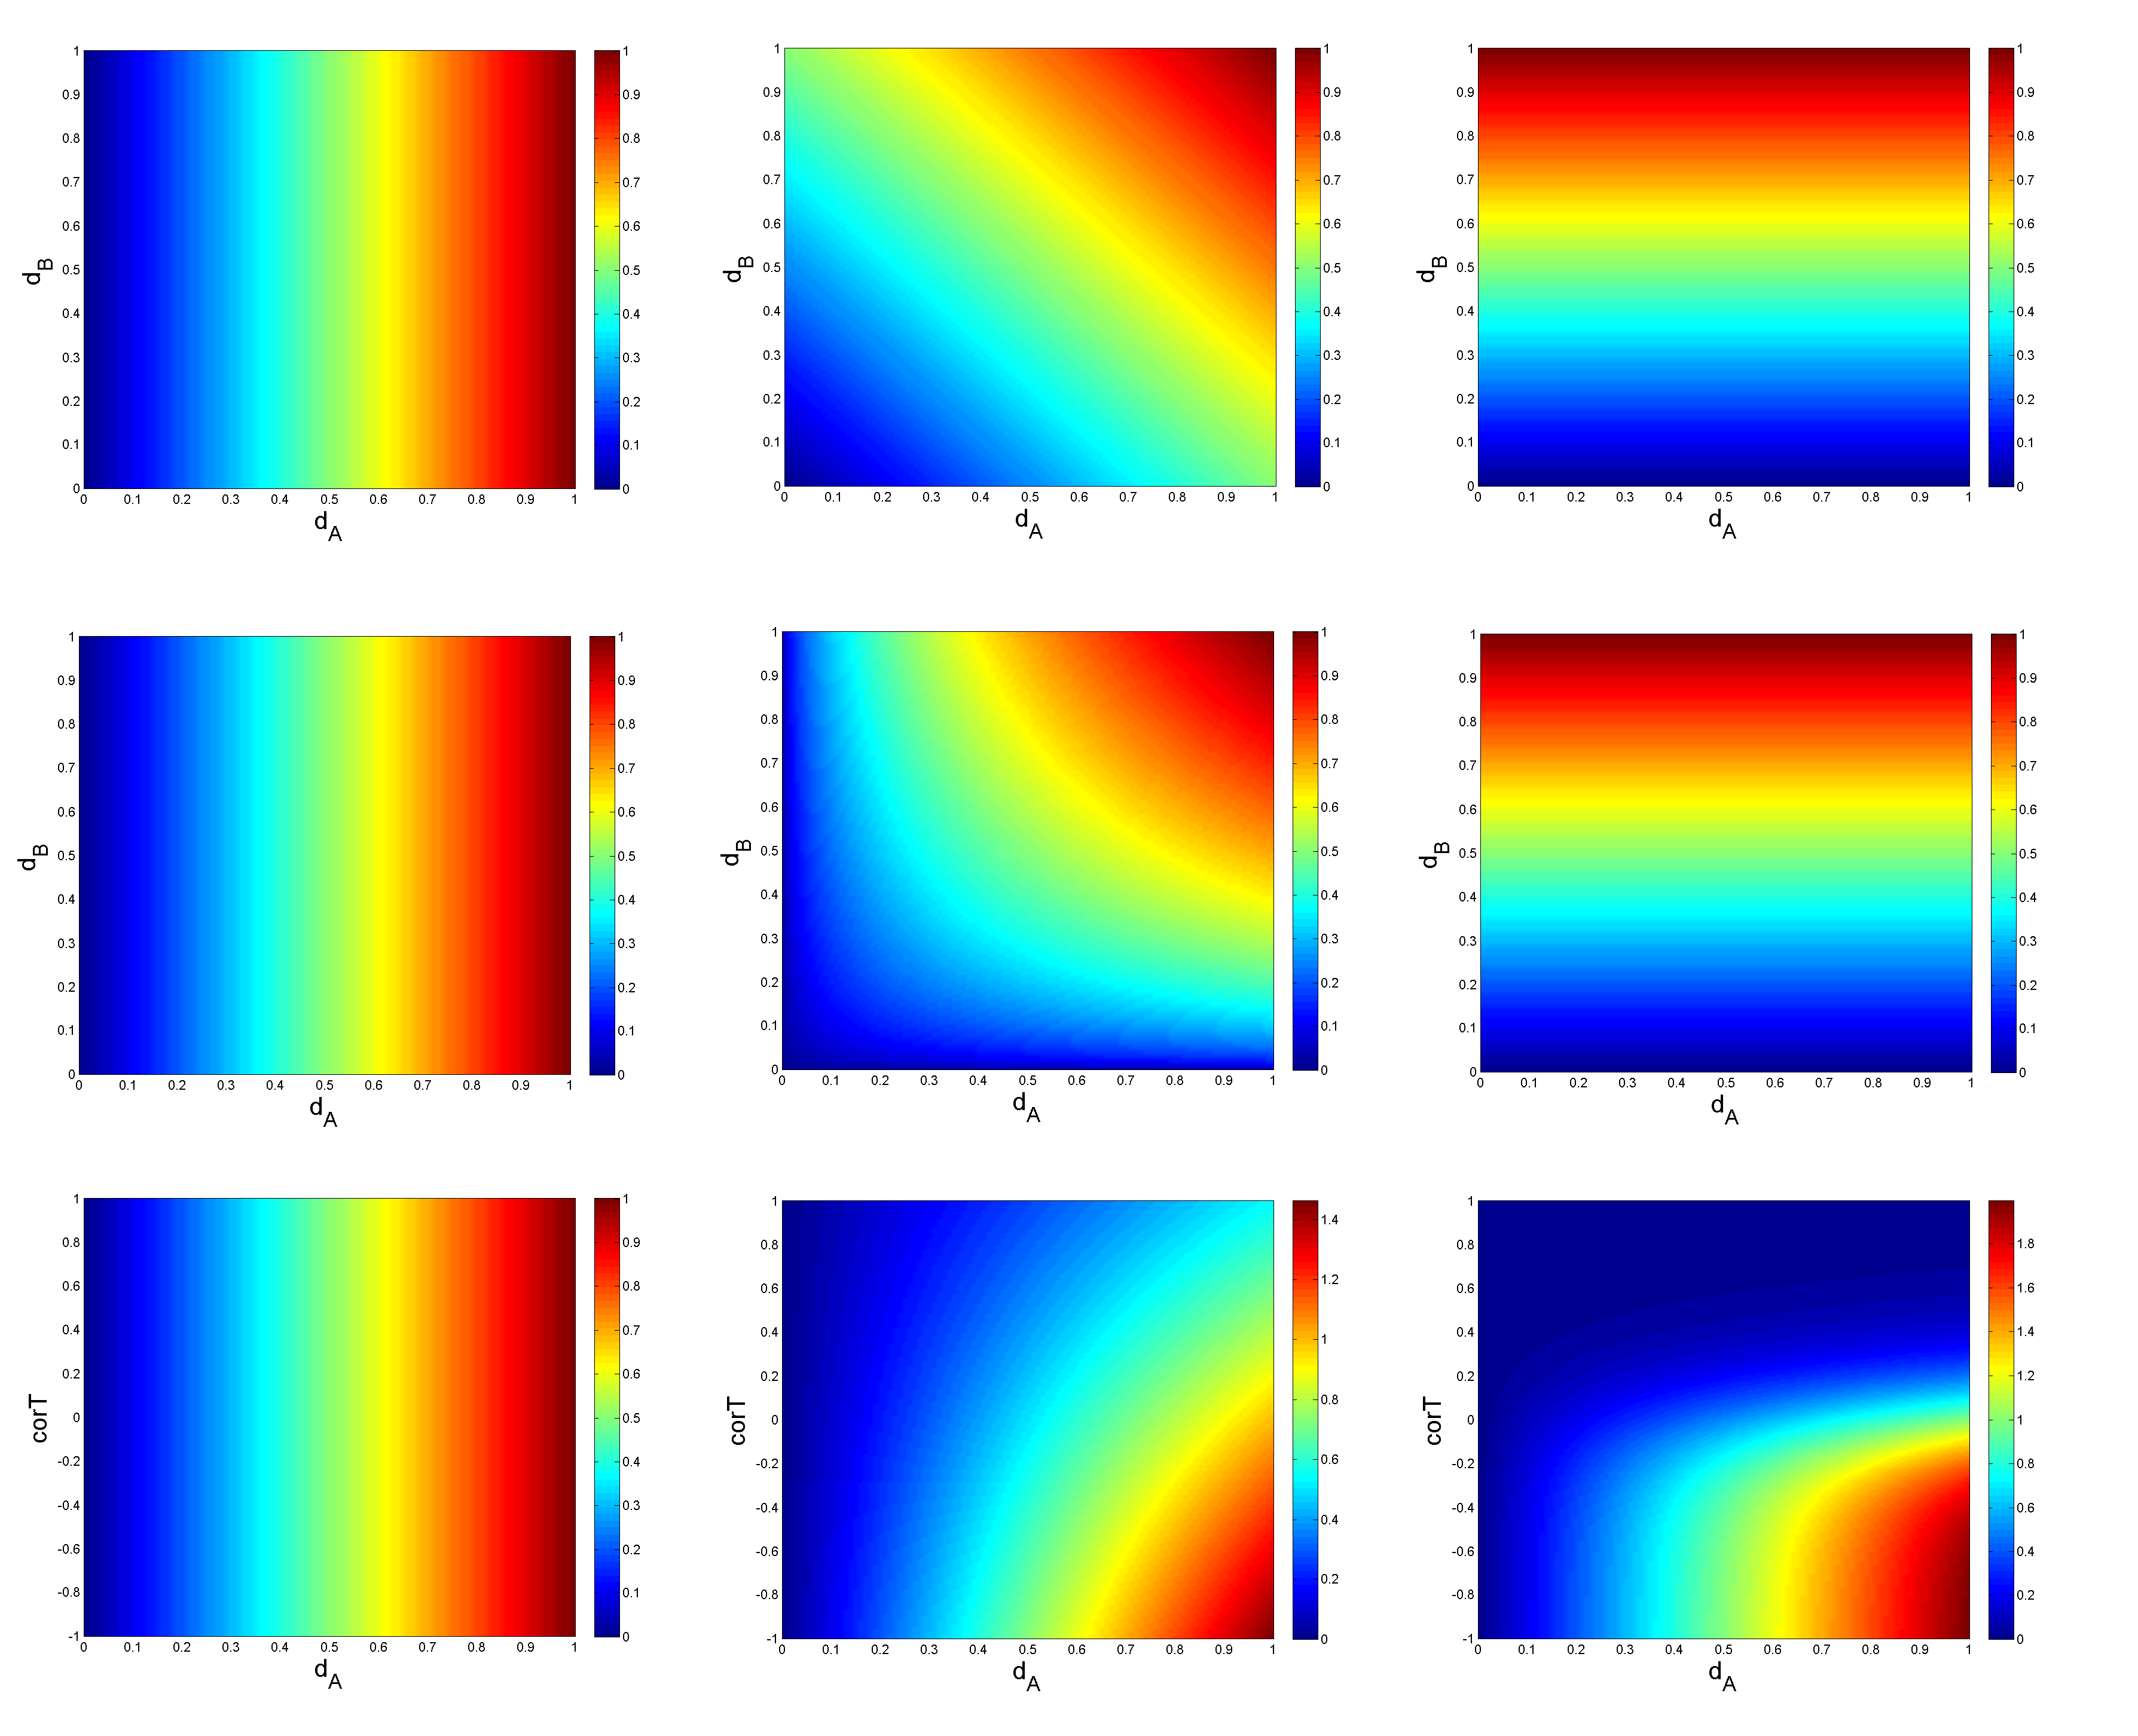
\includegraphics[width=1\linewidth]{images/CombinedMetrics}
	\caption{Contour plot of the resulting combined metrics: $D_{Lin}$ ($1^{st}$ line), $D_{Geom}$ ($2^{nd}$ line) and $D_{Sig}$ ($3^{rd}$ line), for different value of $\alpha$ ($D_{Sig}$: $\alpha=0;1;6$ and $D_{Lin}$ and $D_{Geom}$: $\alpha=0;0.5;1$). For $D_{Sig}$, the first and second dimensions are respectively the amplitude-based metrics $d_A$ and the temporal correlation $corT$; for $D_{Lin}$ and $D_{Geom}$, they correspond to $d_A$ and the behavior-based metric $d_B$.}
	\label{fig:ContourLine}
\end{figure}

%-----------------------------------------------------------------------------
\section{Metric learning}
%\begin{itemize}
%	\item Placer le contexte : travaux réalisés dans le cadre de la classification de données statiques.
%	\item Présenter l'intuition du Metric Learning sur la base des travaux de Weinberger.
%	\item Donner la terminologie (target, imposter, push, pull)
%	\item Objectif : push des imposters et pull des targets
%	\item Formalisation du problème (optimisation)
%	\item Limites:
%	\begin{itemize}
%		\item On apprend les poids d'une distance de Mahalanobis
%		\item L'apprentissage ne prend pas en compte l'aspect multi-modal dans les données
%	\end{itemize}
%\end{itemize}

As our objective is to learn a metric in order to optimize the performance of the $k$-NN classifier, we review first metric learning concepts. Then, we focus on the framework proposed by Weinberger \& Saul for Large Margin Nearest Neighbor ({\sc lmnn}) classification \cite{Weinberger2009}.

\subsection{Review on metric learning work}
In the case of static data, many work have demonstrated that $k$-NN classification performances depends highly on the considered metric and can be improved by learning an appropriate metric \cite{Shental2002,Goldberger2004,Chopra2005}. Metric Learning can be defined as a process that aims to learn a distance from labeled examples by making closer samples that are expected to be similar, and far away those expected to be dissimilar.

\todo[inline]{A faire, avec papier PRL et papier Aurélien Bellet} 
%Similar and dissimilar samples, are inherently task- and application dependent, generally given a priori and fixed during the learning process. From the surge of recent research in metric learning, one can identify mainly two categories: the linear and non linear approaches. The former is the most popular, it defines the majority of the propositions, and focuses mainly on the Mahalanobis distance learning. The latter relies on non linear Metric Learning, although more expressive, the optimization problems are more expensive to solve in general.
%
%Contrary to flat data, Metric Learning for structured data (e.g. sequence, time series, trees, graphs) remains less numerous. While for sequence data most of the works focus on string edit
%distance to learn the edit cost matrix [21, 20], Metric Learning for time series is still in its infancy. Without being exhaustive, major recent proposals rely on weighted variants of dynamic time warping to learn alignments under phase or amplitude constraints [22, 23, 24], or enlarging temporal alignments to learn discriminative matching guided by local variance/covariance [25].


\subsection{Large Margin Nearest Neighbors ({\sc lmnn})}
\label{LMNN}
Let $\textbf{X}=\{\textbf{x}_i,y_i\}_{i=1}^N$ be a set of $N$ static vector samples, ${\textbf{x}_i \in \mathbb{R}^{p}}$, $p$ being the number of descriptive features and $y_i$ the class labels. Weinberger \& Saul proposed in~\cite{Weinberger2009} an approach to learn a dissimilarity metric $D$ for a large margin $k$-NN in the case of static data. 

Large Margin Nearest Neighbor ({\sc lmnn}) approach is based on two intuitions: first, each training sample $\textbf{x}_i$ should have the same label $y_i$ as its $k$ nearest neighbors; second, training samples with different labels should be widely separated. For this, the concept of \textbf{target} and \textbf{imposters} for each training sample $\textbf{x}_i$ is introduced. The training sample $\textbf{x}_i$ is referred as a \textbf{center point}. Target neighbors of $\textbf{x}_i$, noted $j \rightsquigarrow i$, are the $k$ closest $\textbf{x}_j$ of the same class $(y_j=y_i)$, while imposters of $\textbf{x}_i$, denoted, $l \nrightarrow i$, are the $\textbf{x}_l$ of different class $(y_l \neq y_i)$ that invade the perimeter defined by the farthest targets of $\textbf{x}_i$. 
Mathematically, for a sample $\textbf{x}_i$, an imposter $\textbf{x}_l$ is defined by an inequality related to the targets $\textbf{x}_j$: $\forall l, \exists j \in j \rightsquigarrow i /$
\begin{align}
D(\textbf{x}_i,\textbf{x}_l) &\leq D(\textbf{x}_i-\textbf{x}_j) + 1
\end{align}
% ||L(\textbf{x}_i-\textbf{x}_l)||^2 & \leq ||L(\textbf{x}_i-\textbf{x}_j)||^2 + 1 \\
Geometrically, an imposter $\textbf{x}_{l}$ is a sample that invades the target neighborhood plus one unit margin as illustrated in Fig. \ref{fig:TargetImposterRepresentation}. The target neighborhood is defined with respect to an initial metric. Without prior knowledge, L2-norm is often used. Metric Learning by {\sc lmnn} aims to minimize the number of impostors invading the target neighborhood. By adding a margin of safety of one, the model is ensured to be robust to small amounts of noise in the training sample (large margin). The learned metric $D$ pulls the targets $\textbf{x}_j$ and pushes the imposters $\textbf{x}_{l}$ as shown in Fig. \ref{fig:TargetImposterRepresentation}.

\begin{figure}[h!]
	\centering
	\begin{minipage}[b]{0.85\linewidth}		
		\centerline{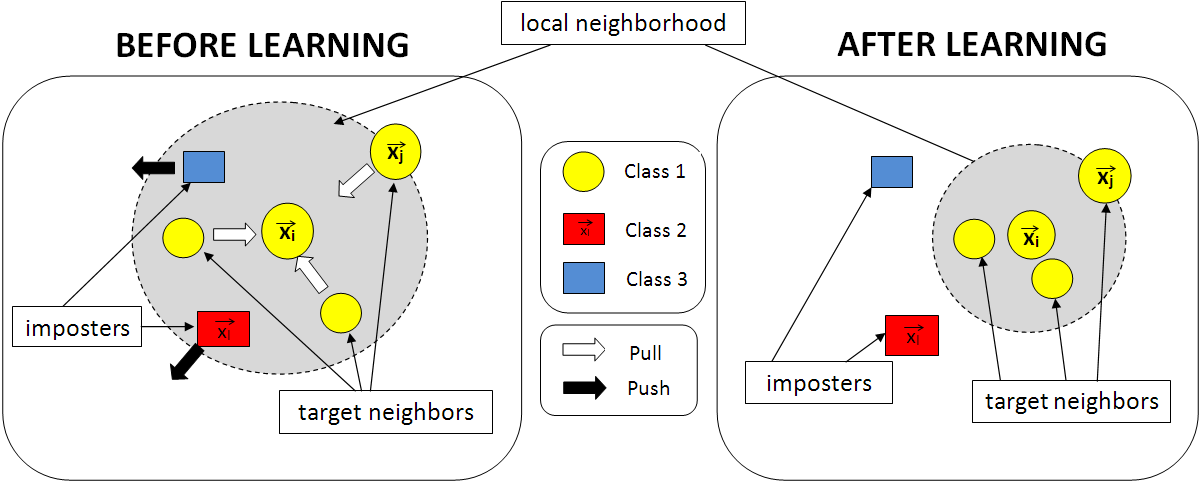
\includegraphics[width=0.8\linewidth]{./images/TargetImposterRepresentationCao}}
	\end{minipage}
	\caption{Pushed and pulled samples in the $k=3$ target neighborhood of $\textbf{x}_i$ before (left) and after (right) learning. The pushed (vs. pulled) samples are indicated by a white (vs. black) arrows (Weinberger \& Saul~\cite{Weinberger2009}).}
	\label{fig:TargetImposterRepresentation}
\end{figure}

{\sc lmnn} approach learns a Mahalanobis distance $D$ for a robust $k$-NN. We recall that the $k$-NN decision rule will correctly classify a sample if its $k$ nearest neighbors share the same label (Section \ref{sec:kNN}). 
The objective of {\sc lmnn} is to increase the number of samples with this property by learning a linear transformation $\textbf{L}$ of the input space ($\textbf{x}_i=\textbf{L}.\textbf{x}_i$) before applying the $k$-NN classification:
\begin{equation}
	D(\textbf{x}_i,\textbf{x}_j) = ||\textbf{L}(\textbf{x}_i,\textbf{x}_j)||_2^2
	\label{eq:lin}
\end{equation}
Commonly, the squared distances can be expressed in terms of the square matrix:
\begin{equation}
\textbf{M} = \textbf{L}'\textbf{L}
\end{equation}
It is proved that any matrix \textbf{M} formed as below from a real-valued matrix \textbf{L} is positive semidefinite (i.e., no negative eigenvalues) \cite{Weinberger2009}. Using the matrix \textbf{M}, squared distances can be expressed as:
\begin{equation}
D^2_\textbf{M}(\textbf{x}_i,\textbf{x}_j) = (\textbf{x}_i-\textbf{x}_j)\textbf{M}(\textbf{x}_i-\textbf{x}_j)
\end{equation}
\noindent The computation of the learned metric $D_\textbf{M}$ can thus be seen as a two steps procedure: first, it computes a linear transformation of the samples $\textbf{x}_i$ given by the transformation $\textbf{L}$; second, it computes the Euclidean distance in the transformed space:
\begin{equation}
D^2_\textbf{M}(\textbf{x}_i,\textbf{x}_j) = D^2(\textbf{L} \textbf{x}_i,\textbf{L} \textbf{x}_j)
\end{equation}
Learning the linear transformation $\textbf{L}$ is thus equivalent to learn the corresponding Mahalanobis metric $D$ parametrized by $\textbf{M}$. This equivalence leads to two different approaches to metric learning: we can either estimate the linear transformation $\textbf{L}$, or estimate a positive semidefinite matrix $\textbf{M}$. {\sc lmnn} solution refers on the latter one.



%\subsection{Intuition}
%%\begin{itemize}
%%	\item Se placer dans le contexte kNN
%%\end{itemize}
%
%Intuitively, the algorithm is based on the simple observation that the kNN decision rule will correctly classify an example if its k-nearest neighbors share the same label. The algorithm attempts to increase the number of training examples with this property by learning a linear transformation of the input space that precedes kNNclassification using Euclidean distances. The linear transformation is derived by minimizing a loss function that consists of two terms. The first term penalizes large distances between examples in the same class that are desired as k-nearest neighbors, while the second term penalizes small distances between exampleswith non-matching labels. Minimizing these terms yields a linear transformation of the input space that increases the number of training examples whose k-nearest neighbors have matching labels. The Euclidean distances in the transformed space can equivalently be viewed as Mahalanobis distances in the original space. We exploit this equivalence to cast the problem of distance metric learning as a problem in convex optimization. Our
Mathematically, it can be formalized as an optimization problem involving two competiting terms for each sample $\textbf{x}_i$: one term penalizes large distances between nearby inputs with the same label (pull), while the other term penalizes small distances between inputs with different labels (push). For all samples $\textbf{x}_i$, this implies a minimization problem:
\begin{equation}
\begin{aligned}
&\displaystyle 		\argmin_{\textbf{M},\xi} \text{  } \underbrace{
	\sum\limits_{i,j \rightsquigarrow i}
	D^2_\textbf{M}(\textbf{x}_i,\textbf{x}_j)
}_{pull}
+
C
\underbrace{
	\sum\limits_{i,j \rightsquigarrow i,l \nrightarrow i} \frac{1+y_{il}}{2}.\xi_{ijl}
}
_{push} \\
&\text{s.t.  } \forall j \rightsquigarrow i, l \nrightarrow i, \\
& D^2_\textbf{M}(\textbf{x}_i,\textbf{x}_l) - D^2_\textbf{M}(\textbf{x}_i,\textbf{x}_j)  \geq 1-\xi_{ijl} \\
& \xi_{ijl} \geq 0 \\
& \textbf{M} \succeq 0
\label{eq:OptimizationProblem}
\end{aligned}
\end{equation}
\noindent where $C$ is a trade-off between the push and pull term and $y_{il}=-1$ if $y_i=y_l$ (same class) and $+1$ otherwise (different classes). Generally, the parameter $C$ is tuned via cross validation and grid search. Similarly to Support Vector Machine ({\sc svm}) approach, slack variables $\xi_{ijl}$ are introduced to relax the optimization problem. 

\subsection{Parallels between {\sc lmnn} and {\sc svm}}
\label{sec:LMNN_SVM}
Many connections can be made between {\sc lmnn} and {\sc svm}: both are convex optimization problem based on a regularized and a loss term. In particular, Do \& al. investigate this relationship and have shown that {\sc svm} can be formulated as a metric learning problem \cite{Do2012}. The Mahalanobis distance $\textbf{M}$ learned by {\sc lmnn} can be expressed as a quadratic mapping $\boldsymbol{\phi}$. For a center point $\textbf{x}_i$, for any sample $\textbf{x}$, we have \cite{Do2012}: 
\begin{align}
	D^2_\textbf{M}(\textbf{x}_i,\textbf{x}) & = D^2(\textbf{L} \textbf{x}_i,\textbf{L} \textbf{x}) \\
	D^2_\textbf{M}(\textbf{x}_i,\textbf{x}) & = \textbf{w}_i^T \boldsymbol{\phi}(\textbf{x}) + b_i
\end{align}	 
\noindent where $\textbf{w}_i$ and $b_i$ are the coefficient of the hyperplane $H_i$ in the quadratic space $\boldsymbol{\phi}$. 

Do \& al. show that {\sc lmnn} can be seen as a set of local {\sc svm} classifiers in the quadratic space induced by $\boldsymbol{\phi}$. For each center point $\textbf{x}_i$, {\sc lmnn} tries in its objective function to have its target neighbors $\textbf{x}_j$ to have small value $\textbf{w}_i^T \boldsymbol{\phi}(\textbf{x}_j) + b_i$, i.e. be at the small distance from the hyperplane $H_i$. Minimizing the target neighbor distances from the hyperplane $H_i$ makes the distance between support vectors and $H_i$ small. Fig. \ref{fig:RelationSVM_LMNN2} gives the equivalent point of view from the original space (Fig. \ref{fig:RelationSVM_LMNN2}(a)) into the quadratic space (Fig. \ref{fig:RelationSVM_LMNN2}(b)). The circle $\textbf{C}_i$ with the center $\textbf{L}\textbf{x}_i$ in Fig. \ref{fig:RelationSVM_LMNN2}(a) corresponds to the hyperplane $H_i$ in Fig. \ref{fig:RelationSVM_LMNN2}(b).

\begin{figure}[h!]
	\centering
	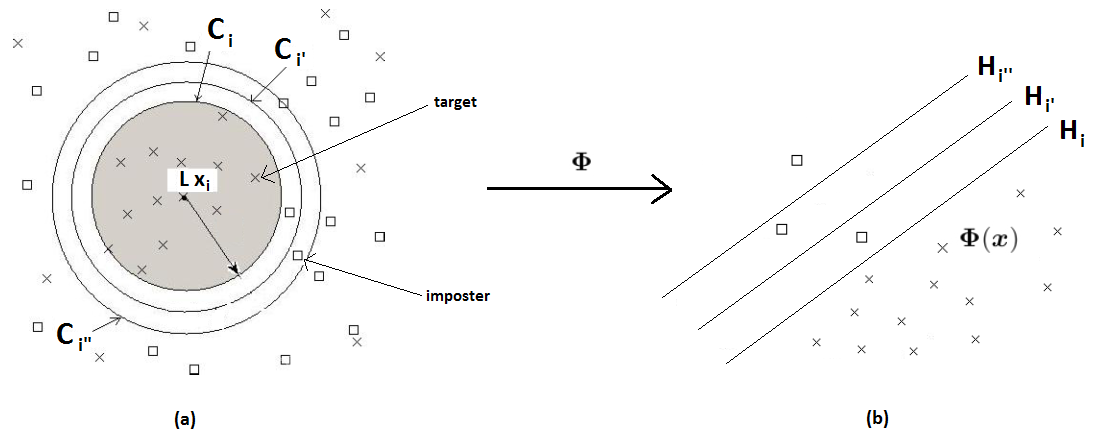
\includegraphics[width=1\linewidth]{images/RelationSVM_LMNN2}
	\caption{(a) Standard {\sc lmnn} model view (b) {\sc lmnn} model view under an {\sc svm}-like interpretation \cite{Do2012}}
	\label{fig:RelationSVM_LMNN2}
\end{figure}


Geometrically, {\sc svm} margin is defined globally with respect to a hyperplane, while {\sc lmnn} margin is defined locally with respect to a center point $\textbf{x}_i$. Fig. \ref{fig:RelationSVM_LMNN}(a) illustrates the different local linear models in the quadratic space. The optimization process of {\sc lmnn} combines the different local {\sc svm} hyperplane by bringing each point $\boldsymbol{\phi }(\textbf{x}_i)$ around a consensus hyperplane $H$.

\begin{figure}[h!]
	\centering
	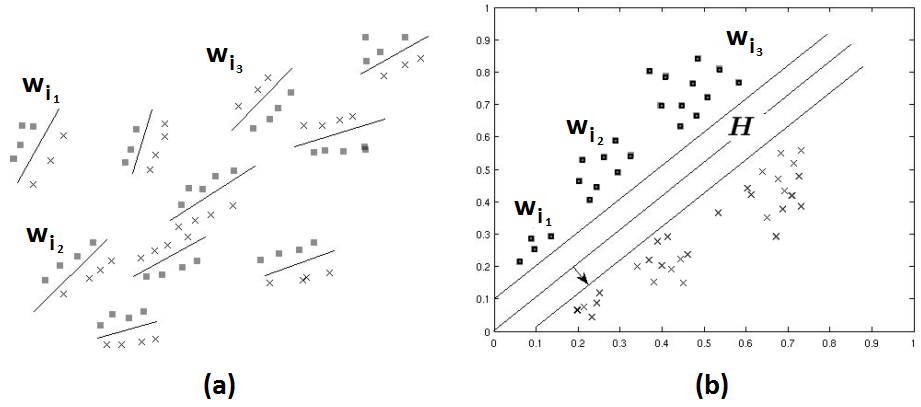
\includegraphics[width=0.9\linewidth]{images/RelationSVM_LMNN}
	\caption{(a) {\sc lmnn} in a local {\sc svm}-like view (b) {\sc lmnn} in an {\sc svm} metric learning view \cite{Do2012}}
	\label{fig:RelationSVM_LMNN}
\end{figure}

From these connections, some authors extends the {\sc lmnn} approach to work in non-linear feature spaces by using the “kernel trick” \todo{ref}. Finally, note that {\sc lmnn} differs from {\sc svm} in which {\sc lmnn} requires no modification for multiclass problems.





%-----------------------------------------------------------------------------
\section{Conclusion of the chapter}
To cope with modalities inherent to time series (amplitude, behavior, frequency, etc.), we review in this chapter several unimodal metrics for time series, in particular, the Euclidean distance $d_A$, the Temporal correlation $d_B$ or the Fourier-based distance $d_F$. 
% Depending on the considered modality (amplitude, behavior, frequency), adapted metrics for time series have been proposed in the literature such as the Euclidean distance $d_A$, the Temporal correlation $d_B$ or the Fourier-based distance $d_F$.
In practice, real time series may be subjected to delays and need to be re-aligned before any analysis task. For that, the Dynamic Time Warping (\textsc{dtw}) algorithm is used in practice. 
% To capture local characteristics, the previous metrics $(d_A, d_B, d_F)$ can be computed on smaller intervals. Many strategies exist such as the dichotomy or the sliding window.
However, these metrics ($d_A, d_B, d_F$) only include one modality. In general, several modalities may be implied and authors proposed to combine temporal metrics together. They mainly combine the Euclidean distance $d_A$ and the Temporal correlation $d_B$. 

As $k$-NN performances is impacted by the choice of the metric, other work propose in the case of static data to learn the metric in order to optimize the $k$-NN classification. In the following, we extend this framework to learn a combined metric for a large margin $k$-NN classifier of time series.

% After that, we will take an insight on Metric Learning approaches which aims to learn a metric that makes closer samples that are expected to be similar, and far away those expected to be dissimilar.


% In the next section, we present a new temporal metric learning framework for a robust nearest neighbors time series classification and give, in Section 4, a solution to learn a holistic temporal metric that combines efficiently several temporal modalities at different scales.


% Local optimal metrics and nonlinear modeling of chaotic time series
% Integration of local and global shape information


%%% Local Variables: 
%%% mode: latex
%%% TeX-master: "../roque-phdthesis"
%%% End: 

\chapter{Time series advanced metrics}
\label{sec:unchapitre}
\minitoc

\noindent Chapeau introductif
\begin{itemize}
	\item Objectif : Trouver une distance, combinaison des distances basiques qui donne une bonne classification $k$-NN sur une base de données.
	\item Pourquoi une distance combinée? Dans le cadre de données réelles, plusieurs modalités peuvent être impliquées (forme, valeur, fréquence), de manière globale ou locale.
	\item Dans le cadre des données réelles, plusieurs composantes/modalités peuvent être impliqués (forme, valeur, fréquence). = attribut (feature) en traitement du signal. Hypothèse : valeur sur une série complète, sur un intervalle ou sur une fenêtre (dans le cadre des métriques à base fréquentielle).
\end{itemize}

%-----------------------------------------------------------------------------
\section{Combined metrics for time series}
\begin{itemize}
	\item Certains travaux dans la littérature propose des combinaisons : linéaire, exponentielle, sigmoïde.
	\item Limites:
	\begin{itemize}
		\item Implique que 2 modalités et au niveau global. Pour intégrer d'autres modalités et à d'autres échelles, il faut changer la formule et ajouter de nouveaux hyper-paramètres à optimiser $\rightarrow$ l'apprentissage de ces paramètres est plus long.
		\item La combinaison est définie a priori
		\item La combinaison est indépendante de la tâche d'analyse.
		\item Pour répondre à ces problèmes, certains auteurs proposent d'apprendre une métrique en vue de la tâche d'analyse considérée (classification, régression, clustering).
	\end{itemize}
\end{itemize}


%-----------------------------------------------------------------------------
\section{Metric Learning: state of the art}
\begin{itemize}
	\item Placer le contexte : travaux réalisés dans le cadre de la classification de données statiques.
	\item Présenter l'intuition du Metric Learning sur la base des travaux de Weinberger.
	\item Donner la terminologie (target, imposter, push, pull)
	\item Objectif : push des imposters et pull des targets
	\item Formalisation du problème (optimisation)
	\item Limites:
	\begin{itemize}
		\item On apprend les poids d'une distance de Mahalanobis
		\item L'apprentissage ne prend pas en compte l'aspect multi-modal dans les données
	\end{itemize}
\end{itemize}

%%% Local Variables: 
%%% mode: latex
%%% TeX-master: "../roque-phdthesis"
%%% End: 

\part*{Conclusion of Part I}
This first part of the manuscript presents a state of the art of classic Machine Learning framework and algorithms to make the classification or the regression of time series. We note that the considered algorithms ($k$-Nearest Neighbors ($k$-NN), Support Vector Machine (SVM)) are based on the comparison of time series through distance measures. 

Considering time series as static data lead to the only comparison based on their amplitude and the same time instant. To take into account other specifities of time series (behavior, frequential components), other metrics (e.g., the temporal correlation $d_B$, the frequential-based distance $d_F$, etc.) and other methods (Dynamic Time Warping {\sc dtw}, dichomotie)  have been proposed to cope with temporal characteristics. 

Learning an adequate metric is a key challenge to well classify time series. Inspired by Metric Learning work for static data, we propose in the following a framework to learn a Multi-modal and Multi-scale Metric for a robust nearest neighbor classifier of time series.

\part{Multi-modal and Multi-scale Time series Metric Learning ({\sc m$^2$tml})}
The first part has enlightened the importance of combining several modalities to make a better analysis (classification, regression) of time series.
% We propose, in this part, a framework to learn this metric. For that, the idea is to introduce a new space representation, the pairwise space, where a vector is a pair of time series described by several unimodal metrics. Then, we formalize the problem of learning the metric as an optimization problem and show its equivalence by solving an adequate Support Vector Machine (SVM) problem. 

In the first chapter, we present the pairwise representation and formalize the optimization problem and its adapted Support Vector Machine ({\sc svm}) approximation. In the second chapter, we present the details of the proposed algorithm: Multi-modal and Multi-scale Time series Metric Learning ({\sc m$^2$tml}). 


\chapter{Pairwise space and $M^2TML$ formalization}
\label{sec:unchapitre}
\minitoc


%\noindent Chapeau introductif
%\begin{itemize}
%	\item Le calcul d'une métrique implique toujours 2 individus. On va proposer un changement d'espace, un nouvel espace : la représentation par paire.
%	\item Le cadre : on suppose que l'on a p métriques.
%\end{itemize}

\fbox{  \parbox{0.9\textwidth}{
		In this chapter, we formalize the problem of the PhD. Our aim is to learn a metric that combines different modalities at different scales. The computation of a metric always implies a pair of samples. In this chapter, we propose to define a new space, the pairwise space in which a pair of time series is embedded as a vector described by the different metrics at different scales. Inspired from the Metric Learning framework, we transpose the metric learning problem in the pairwise space to propose a Multi-Modal and Multi-scale Time series Metric Learning framework for the classification and regression of time series.
	}  }

%---------------------------------------------------------------------------
\section{Pairwise space representation}
%\begin{itemize}
%	\item Changement de l'espace
%	\item Normalisation de l'espace des paires
%	\item Label des pairwise
%\end{itemize}

\noindent \textbf{Pairwise embedding} \\
Let  $d_1, ..., d_h ..., d_p$ be $p$ given dissimilarity metrics that allow to compare samples. The computation of a metric always takes into account a pair of samples. We introduce a new space representation referred as the pairwise space. In this new space, illustrated in Figure \ref{fig:PairwiseEmbedding}, a vector $\textbf{x}_{ij}$ represents a pair of samples $(\textbf{x}_i,\textbf{x}_j)$ described by the $p$ basics metrics $d_h$: $\textbf{x}_{ij}=[d_1(\textbf{x}_i,\textbf{x}_j), ..., d_p(\textbf{x}_i,\textbf{x}_j)]^T$.
%		\begin{equation*}		
%			\textbf{x}_{ij}
%			=
%			\begin{bmatrix}
%		        d_1(\textbf{x}_i,\textbf{x}_j) 	\\
%		        ... 			\\
%		       	d_p(\textbf{x}_i,\textbf{x}_j)
%		     \end{bmatrix}	    	     
%		\end{equation*}


\begin{figure}[h!]
	\begin{minipage}[b]{1.0\linewidth}
		\centering
		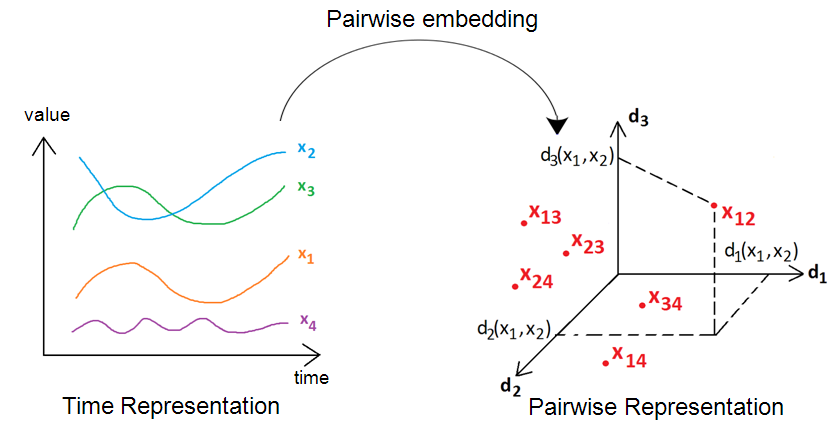
\includegraphics[width=0.8\linewidth]{images/PairwiseEmbedding}
	\end{minipage}
	\caption{Example of embedding of time series $\textbf{x}_i$ from the temporal space (left) into the pairwise space (right). In this example, a pair of time series $(\textbf{x}_1, \textbf{x}_2)$ is projected into the pairwise space as a vector $\textbf{x}_{12}$ described by $p=3$ basic metrics: $\textbf{x}_{12} = [d_1(\textbf{x}_1, \textbf{x}_2), d_2(\textbf{x}_1, \textbf{x}_2), d_3(\textbf{x}_1, \textbf{x}_2)]^T$.}
	\label{fig:PairwiseEmbedding}
\end{figure}

A combination function $D$ of the metrics $d_h$ can be seen as a function in this space. We propose in the following to use a linear combination of $d_h$: $D_w(\textbf{x}_i,\textbf{x}_j) = \sum_h w_h.d_h(\textbf{x}_i,\textbf{x}_j)$. Its pairwise notation is:
\begin{equation}
D_w(\textbf{x}_{ij})=\textbf{w}^T.\textbf{x}_{ij}
\end{equation}



\noindent \textbf{Pairwise label} \\
In classification problems, each pair $(\textbf{x}_i,\textbf{x}_j)$ is labeled:
\begin{equation}
	y_{ij} = 
	\left\{
	\begin{split}
	-1 \text{\quad if } y_i = y_j\\ 
	+1 \text{\quad if } y_i \neq y_j
	\end{split}
	\right.
\end{equation}
In regression problems, two approaches are possible. The first one aims to discretize by binning the label $y_i$ into $Q$ intervals as illustrated in Fig. ??. Each interval becomes a class which associated value can be set for example as the mean or median value of the interval. Then, the practitioner use the classification framework.

\missingfigure{Mettre une figure ici montrant la discretization. Faire 2 figures, la 1ère montre dans le domaine temporal et son équivalent en classe. La 2ème est une figure entrée/sortie}  

\noindent The second technic consider a tube of size $\epsilon$ around each value of $y_i$.

%---------------------------------------------------------------------------
\subsection{Interpretation of the pairwise space}
\begin{itemize}
	\item Proximity to the origin (les individus sont identiques)
	\item Proximity of 2 pairwise points in the pairwise space 
	\item Norm in the pairwise space
	\item Representation of combined metric in the pairwise space
\end{itemize}
%%% Local Variables: 
%%% mode: latex
%%% TeX-master: "../roque-phdthesis"
%%% End: 
If $\textbf{x}_{ij}=\textbf{0}$ then $\textbf{x}_{j}$ is identical to $\textbf{x}_{i}$ according to all metrics $d_h$.

%---------------------------------------------------------------------------
\subsection{Pros \& Cons}
\begin{itemize}
	\item perte de la classe initiale des individus. L'information qui nous reste est : les 2 individus sont de la même classe ou sont de classes différentes.
\end{itemize}



\section{$M^2TML$: LP optimization problem}
\begin{itemize}
	\item Formaliser le problème sous forme d'un problème d'optimisation sous contraintes
\end{itemize}

\section{$M^2TML$: QP optimization problem}
\begin{itemize}
	\item Passer de la forme LP (forme primale) et par transformation, arriver à la forme duale
	\item Montrer les similitudes avec la résolution SVM
	\item Montrer que l'on peut kerneliser la méthode
\end{itemize}


\section{$M^2TML$: SVM approximation}
\begin{itemize}
	\item Faire remarquer que le problème LP ressemble à un problème SVM
	\item Faire la démonstration de l'équivalence (ou mettre la démonstration en annexe).
	\item Expliquer les différences entre la résolution LP/QP et la résolution SVM. (ajout de sur-contraintes dans le problème SVM)
	\item Expliquer pourquoi on va préférer le cadre SVM. Expliquer mathématiquement et avec des interprétations géométriques. 
	\item Cadre connu
	\item Utilisation de librairie standard de Machine Learning
	\item Extension directe à l'apprentissage de métrique non linéaire grâce au kernel trick
\end{itemize}

\chapter{$M^2TML$: formalization}
\label{sec:unchapitre}
\minitoc

\noindent Chapeau introductif
\begin{itemize}
	\item Rappeler : quel problème on résout : pull des targets et push des individus de classes différentes
	\item Formaliser le problème général avec D
\end{itemize}

\section{LP optimization problem}
\begin{itemize}
	\item Formaliser le problème sous forme d'un problème d'optimisation sous contraintes
\end{itemize}

\section{QP optimization problem}
\begin{itemize}
	\item Passer de la forme LP (forme primale) et par transformation, arriver à la forme duale
	\item Montrer les similitudes avec la résolution SVM
	\item Montrer que l'on peut kerneliser la méthode
\end{itemize}


\section{SVM approximation}
\begin{itemize}
	\item Faire remarquer que le problème LP ressemble à un problème SVM
	\item Faire la démonstration de l'équivalence (ou mettre la démonstration en annexe).
	\item Expliquer les différences entre la résolution LP/QP et la résolution SVM. (ajout de sur-contraintes dans le problème SVM)
	\item Expliquer pourquoi on va préférer le cadre SVM. Expliquer mathématiquement et avec des interprétations géométriques. 
	\item Cadre connu
	\item Utilisation de librairie standard de Machine Learning
	\item Extension directe à l'apprentissage de métrique non linéaire grâce au kernel trick
\end{itemize}

%%% Local Variables: 
%%% mode: latex
%%% TeX-master: "../roque-phdthesis"
%%% End: 

\chapter{$M^2TML$: implementation}
\label{sec:unchapitre}
\minitoc

\noindent Chapeau introductif :
\begin{itemize}
	\item Quel problème on résout?
	\item Donner les étapes principales de résolution (sous forme de puces). Cela doit rester général, clair et concis.
	\item Développer dans chaque section les puces énumérés précédemment.
\end{itemize}

%---------------------------------------------------------------------------
\section{Projection in the pairwise space}
\begin{itemize}
	\item Projection
	\item Log normalization
\end{itemize}
\noindent \textbf{Pairwise space normalization} \\
This operation is performed to scale the data within the pairwise space and ensure comparable ranges for the $p$ basic metrics $d_h$. In our experiment, we use dissimilarity measures with values in $[0;+\infty[$. Therefore, we propose to Z-normalize their log distributions. \\

%---------------------------------------------------------------------------
\section{M-NN M-diff strategy}
\begin{itemize}
	\item Expliquer les différentes stratégies (k-NN VS All / M-NN VS M-diff / k-NN VS Imposters)
	\item Expliquer pourquoi on va choisir une stratégie M-NN VS M-diff
\end{itemize}


%---------------------------------------------------------------------------
\section{Radius normalization}
\begin{itemize}
	\item Expliquer le problème de la non-homogénéité des radius.
	\item Expliquer comment on résout ce problème par une normalisation des radius de chaque voisinage.
\end{itemize}


%---------------------------------------------------------------------------
\section{Solving the SVM problem}
\begin{itemize}
	\item Expliquer l'apprentissage avec le SVM.
	\item Utilisation de la version L1 du SVM pour avoir une solution sparse.
\end{itemize}


%---------------------------------------------------------------------------
\section{Definition of the dissimilarity measure}
\begin{itemize}
	\item Produit scalaire
	\item Papier PR : norme pondérée x fonction exponentielle
	\item Version Sylvain : norme x fonction exponentielle?
\end{itemize}


%---------------------------------------------------------------------------
\section{Extension to regression problem}
\textit{(To do)}

%---------------------------------------------------------------------------
\section{Extension to multivariate problem}
\textit{(To do)}



%%% Local Variables: 
%%% mode: latex
%%% TeX-master: "../roque-phdthesis"
%%% End: 

\chapter{Experiments}
\label{sec:unchapitre}
\minitoc


%\noindent Chapeau introductif
%\begin{itemize}
%	\item Application sur des bases de séries temporelles univariés de la littérature (Keogh)
%	\item Données Schneider? ou Expliquer les problématiques de Schneider
%\end{itemize}
\fbox{  \parbox{0.9\textwidth}{
		In this chapter, we evaluate the efficiency of the proposed {\sc m}$^2${\sc tml} algorithm on public datasets for classification problems of univariate time series. First, we describe the datasets. Then, we detail the experimental protocol. Finally, we present and discuss the obtained results.
	}  }
%-----------------------------------------------------------------------------
\section{Description}
The efficiency of the  learned multi-modal and multi-scale dissimilarities $D$ and $D_{\mathcal{H}}$ is evaluated through  a $1$-NN classification on 30 public datasets\footnote{PowerCons:   \url{https://archive.ics.uci.edu/ml/datasets/Individual+household+electric+power+consumption}, {\sc bme} and {\sc umd}:  \url{http://ama.liglab.fr/~douzal/tools.html}.} \cite{Keogh2011}. 
The $1$-NN classifier is used to make the results comparable with the results of the UCR time series data mining archive\footnote{Note: the datasets and results are the ones before the update of August 2015}.
%\footnote{\url{http://www.cs.ucr.edu/~eamonn/time_series_data/}}
Time series come from several fields (simulated data, medical data, electrical data, etc.), are from variable lengths (from small ($q=24$) to long lengths ($q=1882$)) and the number of classes to discriminate evolves between 1 and 37 classes. Note that some of the datasets have a small number of time series in the training set ($n < 30$) and others have a large number of time series in the training set ($n > 100$). The results using standard metrics (Euclidean distance, Dynamic time warping) show both easy and challenging classifications problems, the latter being opened for improvements. 

Table \ref{tab:DatasetDescription} gives a description of the datasets considered in the experiments and Fig. \ref{fig:dataset} gives the temporal representation for some of the datasets. Note that for some datasets (\textit{e.g.}, SonyAIBO, ECG200, FaceFour, PowerConsumption), it is visually difficult to  discriminate the classes using one modality (value, behavior, frequential).

\begin{table}[h!]
	\small
	\begin{center}
		\renewcommand{\arraystretch}{1}
		\resizebox{0.6\textwidth}{!}{
			\begin{tabular}{lcccc}
				\hline
				Dataset    	& Nb. Class & Nb. Train 
				& Nb. Test  & TS length\\
				\hline
				1 ItalyPowerD 	 	& 2 & 67  & 1029 & 24  \\
				2 CinCECGtorso		& 4 & 40  & 1380 & 1639\\
				3 BME				& 3 & 300 & 1500 & 128 \\
				4 ECG200			& 2 & 100 & 100  & 96  \\
				5 SonyAIBOII		& 2 & 27  & 953  & 65  \\
				6 Coffee			& 2 & 28  & 28   & 286 \\
				7 ECG5Days			& 2 & 23  & 861  & 136 \\
				8 SonyAIBO			& 2 & 20  & 601  & 70  \\
				9 Adiac				& 37& 390 & 391  & 176 \\
				10 Beef				& 5 & 30  & 30   & 470 \\
				11 Trace 			& 4 & 100 & 100  & 275 \\
				12 CBF 				& 3 & 30  & 900  & 128 \\
				13 CC				& 6 & 300 & 300  & 60  \\	
				14 DiatomSizeReduc 	& 4 & 16  & 306  & 345 \\
				15 Symbols 			& 6 & 25  & 995  & 398 \\						
				16 GunPoint			& 2 & 50  & 150  & 150 \\
				17 FacesUCR			& 14& 200 & 2050 & 131 \\
				18 TwoLeadECG 		& 2 & 23  & 1139 & 82  \\
				19 UMD				& 3 & 360 & 1440 & 150 \\									
				20 MoteStrain		& 2 & 20  & 1252 & 84  \\				
				21 Lighting2		& 2 & 60  & 61   & 637 \\
				22 OliveOil			& 4 & 30  & 30   & 570 \\				
				23 FISH				& 7 & 175 & 175  & 463 \\				
				24 FaceFour			& 4 & 24  & 88   & 350 \\
				25 SwedishLeaf		& 15& 500 & 625  & 128 \\
				26 MedicalImages	& 10& 381 & 760  & 99 \\				
				27 Lighting7		& 7 & 70  & 73   & 319 \\
				28 PowerCons		& 2 & 73  & 292  & 144 \\						
				29 OSULeaf			& 6 & 200 & 242  & 427 \\
				30 InlineSkate		& 7 & 100 & 550  & 1882\\	    
				\hline
			\end{tabular}
		}
	\end{center}
	% \vspace*{-0.3cm}
	\caption{Dataset table description providing the number of classes (Nb. Class), the number of time series for the training (Nb. Train) and the testing (Nb. Test) sets, and the length of each time series (TS length).}
	\label{tab:DatasetDescription}
\end{table}

\begin{figure}[h!]
	\centering
	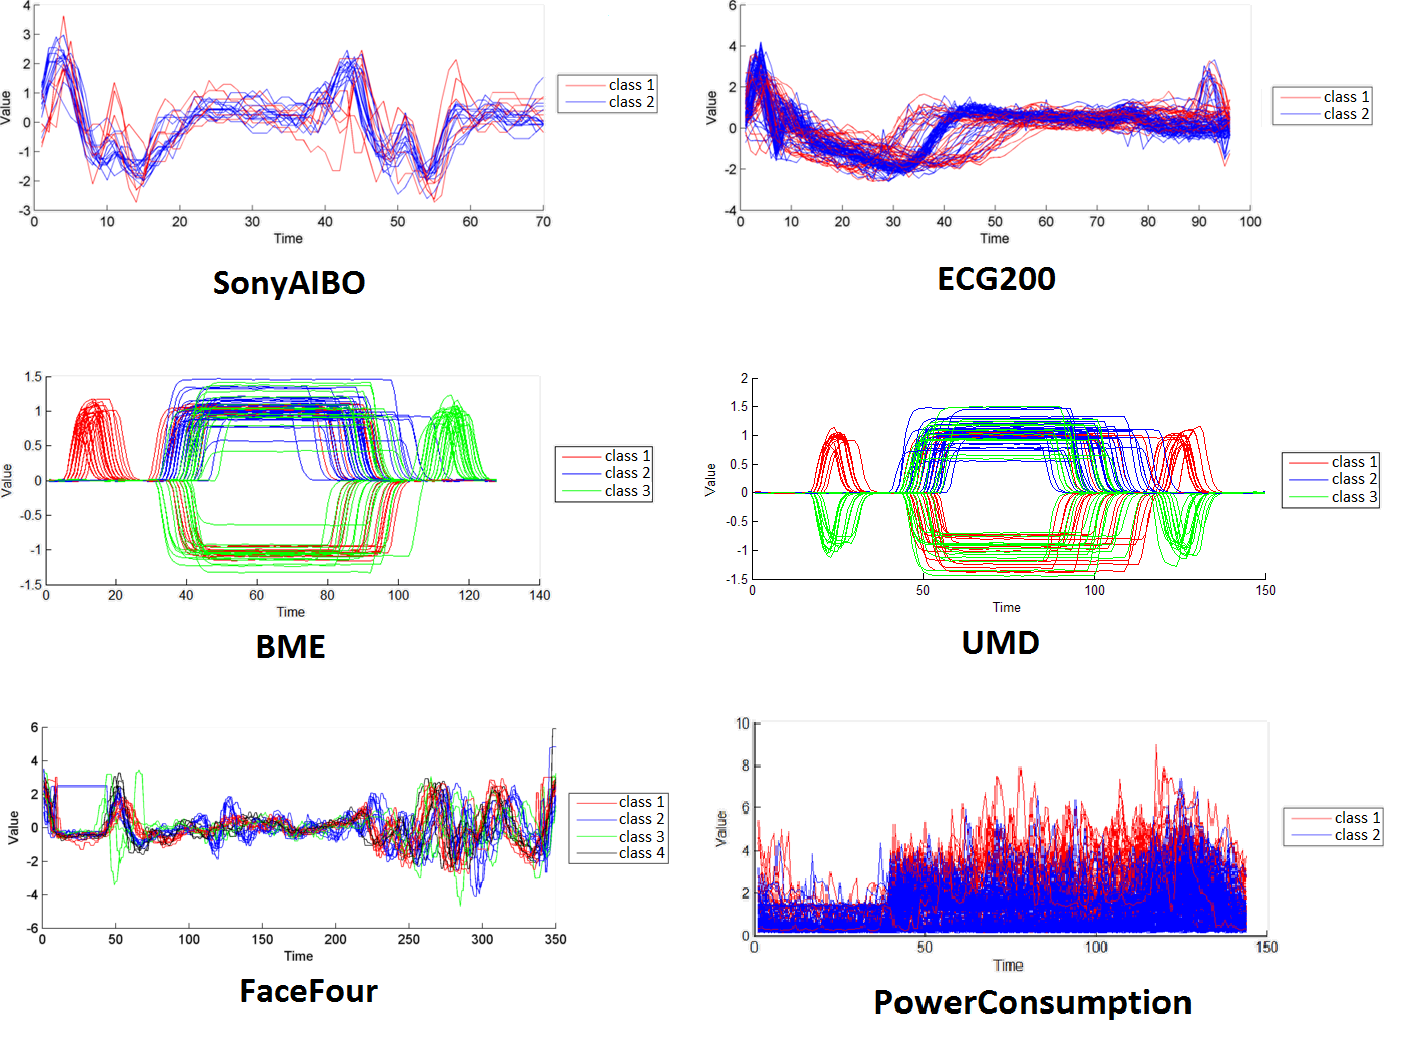
\includegraphics[width=0.95\linewidth]{images/dataset_exp}
	\caption{Temporal representation of some datasets (SonyAIBO, ECG200, BME, UMD, FaceFour, PowerConsumption) considered in the experiments.}
	\label{fig:dataset}
\end{figure}

\noindent The results of the learned metrics $D$ and $D_{\mathcal{H}}$ are compared to those of three \textit{a priori} combined metrics $D_{Lin}, D_{Geom}, D_{Sig}$ (Eqs. \ref{eq:DLin}, \ref{eq:DGeom}, \ref{eq:DSig}) and five alternative uni-modal metrics covering: 
\begin{enumerate}
	\item The standard  Euclidean distance $d_A$ (Eq. \ref{eq:A}) and Dynamic time warping\footnote{In this chapter, the term {\sc dtw} denotes the classically value-based metric computed after an alignment of the time series obtained with the {\sc dtw} algorithm with a value-based cost function.} {\sc dtw} (Eq. \ref{eq:DTW})
	\item The behavior-based measures  $d_B$ (Eq. \ref{eq:B}) and $d_{B-\mbox{\sc dtw}}$ its counterpart  for asynchronous time series, that is $d_B$ is evaluated once time series are synchronized using dynamic programing
	\item The frequential-based metric  $d_F$ (Eq. \ref{eq:F}). 
\end{enumerate}

\begin{table}[h!]
	\small
	\centering
	\renewcommand{\arraystretch}{0.85}
	\resizebox{1\textwidth}{!}{
		\setlength{\tabcolsep}{1pt}
		\begin{tabular}{llll}
			\hline
			Symbol & Name & Equation reference & Description \\
			\hline
			$d_A$ 				& Value-based dissimilarity			& Eq. \ref{eq:A} 				& Euclidean distance\\
			$d_B$ 				& Behavior-based dissimilarity 		& Eq. \ref{eq:B} 				& Behavior metric based on cort\\
			\textsc{dtw}		& Dynamic time warping 				& Eqs. \ref{eq:DTW} \& \ref{eq:A}& Euclidean distance after alignment\\
			$d_{B-\mbox{\sc dtw}}$ & Behavior-based aligned dissimilarity & Eqs. \ref{eq:DTW} \& \ref{eq:B}& Behavior metric based on cort after alignment\\
			$d_F$ 				& Frequential-based dissimilarity 	& Eq. \ref{eq:F} 				& Frequential  metric based on Fourier transform\\
			$D_{Lin}$ 			& Linear combined metric 			& Eq. \ref{eq:DLin} 			& Combines $d_A$ and $d_B$ (resp. \textsc{dtw} and $d_{B-\mbox{\sc dtw}}$) \\
			$D_{Geom}$ 			& Geometric combined metric 		& Eq. \ref{eq:DGeom} 			& Combines $d_A$ and $d_B$ (resp. \textsc{dtw} and $d_{B-\mbox{\sc dtw}}$) \\
			$D_{Sig}$ 			& Sigmoid combined metric 			& Eq. \ref{eq:DSig} 			& Combines $d_A$ and $d_B$ (resp. \textsc{dtw} and $d_{B-\mbox{\sc dtw}}$) \\
			$D$ 				& Linear learned metric 				& Eq. \ref{eq:dissimilarity_learn} 			 & \textsc{m$^2$tml} linear combined metric\\ 
			$D_{\mathcal{H}}$  	& Non-linear learned metric 			& Eq. \ref{eq:dissimilarity_learn_NonLinear} & \textsc{m$^2$tml} non-linear combined metric with a Gaussian kernel\\
			\hline
		\end{tabular}}
		\caption{Considered metric in the experiments}
		\label{tab:metric}
	\end{table}
	
\noindent Table \ref{tab:metric} recalls briefly the considered metrics in the experiments. The \textit{a priori} combined metrics ($D_{Lin}, D_{Geom}, D_{Sig}$) rely, on 2 log-normalized dissimilarities $d_{A}$, $d_{B}$ (resp. {\sc dtw}, $d_{B-\mbox{\sc dtw}}$ for asynchronous time series). The alternative metrics and the \textit{a priori} combined metrics are evaluated  as usual by involving all time series elements ({\it i.e.}, at the global scale). For $D$ and $D_{\mathcal{H}}$, we consider a 21-dimensional embedding space  $\mathcal{E}$ that relies, for synchronous (resp. asynchronous) data, on 3 log-normalized dissimilarities $d_{A}^{s}$, $d_{B}^{s}$ (resp. {\sc dtw}$^{s}$, $d_{B-\mbox{\sc dtw}}^{s}$), and $d_{F}^{s}$, at 7 temporal granularities $s \in \{0,...,6\}$ obtained by binary segmentation, described in Section \ref{sec:Pairwise_embedding}.

%-----------------------------------------------------------------------------
\section{Experimental protocol}
The different metrics can be split into two categories. For those without parameters to tune ($d_A$, \textsc{dtw}), the $1-$NN classifier is applied directly on the test set. For those that require to tune parameters ($d_B$, $d_{B-\mbox{\sc dtw}}$, $D_{Lin}$, $D_{Geom}$, $D_{Sig}$, $D$, $D_{\mathcal{H}}$), we recall briefly the grid search and cross-validation procedure (Section \ref{sec:model_selection}). When a learning algorithm requires to tune some parameters, to avoid overfitting, the training set can be divided into two sets: a learning and a validation set. The model is learnt for each combination of parameters (grid search) on the learning set and evaluated on the validation set. The model with the lowest error on the validation set is retained. An other alternative is cross-validation, which partitions the training set into $v$ folds, performs the learning on one subset, and validates on the $v-1$ other subsets. To take into account of variability within the data, multiple rounds of cross-validation are performed using different partitions, and the validation results are averaged over the rounds. Note that for unbalanced datasets in classification problems, it is recommended to use stratified sampling. Table \ref{tab:param} resumes the parameter ranges for each metric. We recall that the parameters retained are those that:
\begin{itemize}
	\item[-] \textbf{First}, minimize the average classification error on the validation set.
	\item[-] \textbf{Secondly}, in the case of multiple solutions leading to equal performances, the most discriminant one is retained (\textit{i.e.}, making closer pull pairs and far away push pairs). Precisely, it minimizes the ratio $\frac{d_{intra}}{d_{inter}}$ where $d_{intra}$ and $d_{inter}$ stands respectively to the mean of all intraclass and interclass distances.
\end{itemize} 
\noindent As $D$ and $D_{\mathcal{H}}$ involves several parameters to be tuned, we detail hereafter the procedure. The combined metrics $D$ and $D_{\mathcal{H}}$  ($\kappa$ as the Gaussian kernel) are learned respectively under $L_1$ and $L_2$ regularization, using \textsc{liblinear}  and \textsc{libsvm} libraries \cite{Fan2008,Hsu2008}. The parameters are estimated on a validation set by line/grid search. A cross-validation and stratified sampling for unbalanced datasets are used.  Particularly, for each  couple ($r$, $\lambda$) $r \in \{1, 4, 10\}$ and $\lambda \in \{0, 10, 30\}$, the pairwise {\sc svm} parameters ($C,\alpha, \gamma$) are learned by grid search as indicated in Table \ref{tab:param}. 

\begin{table}[h!]
	\small
	\centering
	\renewcommand{\arraystretch}{0.85}
	\resizebox{1\textwidth}{!}{
		\setlength{\tabcolsep}{1pt}
		\begin{tabular}{lccl}
			\hline
			Dissimilarity & Parameter & Ranges & Description\\
			\hline
			$d_{B}$, $d_{B-\mbox{\sc dtw}}$ & $r$       & $\{1, 2, 3, , \ldots, q-1\}$ 					& Order of behavior-based metric\\
			$D_{Lin}, D_{Geom}, D_{Sig}$ & $\beta$ & $\{0,0.1, \ldots, 1\}$ 					& Trade-off between value and behavior components\\
			$D$, $D_{\mathcal{H}}$  & $\lambda$ & $\{0, 10, 30\}$ 								& Strength of the '{\it push}' term \\
			$D$, $D_{\mathcal{H}}$  & $r$       & $\{1, 4, 10\}$ & Order of behavior-based metrics\\			
			$D$, $D_{\mathcal{H}}$  & $C$       & $\{10^{-3}, 0.5, 1, 5, 10, 20, 30, ..., 150\}$& Parameter of \textsc{svm}\\
			$D$, $D_{\mathcal{H}}$  & $\alpha$  & $\{1,2,3\}$     								& Size of the $m=\alpha.k$ neighborhood\\
			$D_{\mathcal{H}}$       & $\gamma$  & $\{10^{-3}, 10^{-2}, \ldots, 10^{3}\}$ 		& Parameter of the Gaussian kernel\\
			\hline
		\end{tabular}}
		\caption{Parameter ranges}
		\label{tab:param}
\end{table}
	
Note that the temporal order $r$ for the behavior-based metrics $d_B$ is noise-dependent, typically 1 is retained for noise-free data. The parameter $\lambda$ corresponds to the strength of the '{\it push}' term; precisely, if no, moderate or  strong '{\it push}'  is required during the training process, a $\lambda$ value of  0, 10 and 30 is learned, respectively. 
%-----------------------------------------------------------------------------
\newpage
\section{Results and discussion}
In this section, we first present a summary table of the quantitivative results obtained in the experiment. Secondly, we present an analysis of the performances of the different metrics. Finally, we present the ability of our proposed approach \textsc{m$^2$tml} to extract discriminative features.

\subsection{Results}
Table \ref{tab-resu} reports the 1-NN classification test errors based on uni-modal metrics  (first 5 columns), on three \textit{a priori} combined metrics ($D_{Lin}, D_{Geom}, D_{Sig}$) and on  $D$ and $D_{\mathcal{H}}$. The results for each dataset that are statistically and significantly better than the best performance are indicated in bold (Z-test at  5\% risk detailed in Section \ref{sec:ClassificationEvaluation}). The last column '{\sc warp}' indicates the synchronous (\checkmark) or asynchronous ($\times$) data type. \\ 
Data that need '{\sc warp}' are situated above the line. For each type of delay ('{\sc warp}' or non-'{\sc warp}'), the datasets are ordered from the less challenging datasets according to the performance of the classically used distances ($d_A$ or {\sc dtw}) to the most challenging datasets.

\begin{table}[h!]
	\small
	\centering
	\renewcommand{\arraystretch}{0.8}
	\resizebox{1\textwidth}{!}{
		\setlength{\tabcolsep}{1pt}
		\begin{tabular}{|l|ccccc|ccc|ccc|}
			\hline
			& \multicolumn{5}{c|}{Alternative uni-modal metrics} & \multicolumn{3}{c|}{A priori combinations} & \multicolumn{2}{c}{{\sc m}$^2${\sc tml}} & {\sc warp}  \\
			\cline{2-12} 
			Dataset & $d_A$ & $d_B$ & $d_F$ & $\mbox{\sc dtw}$ & $d_{B-\mbox{\sc dtw}}$ & $D_{Lin}$ & $D_{Geom}$ & $D_{Sig}$ & $D (\lambda^*)$ & $D_{\mathcal{H}} (\lambda^*)$ & {\sc warp}  \\
			\hline
			1 ItalyPowerD     	& 0.045 & \textbf{0.028}& 0.078 & 0.050 & 0.055    & \textbf{0.028} & \textbf{0.028} & \textbf{0.030} & \textbf{0.034} (0) & 0.046 (0) & $\times$  \\
			2 CinCECGtorso        & 0.103 & 0.367 & 0.167 & 0.349 & 0.367  & \textbf{0.094} & \textbf{0.094} & \textbf{0.093} & \textbf{0.092} (0)  & \textbf{0.088} (0) & $\times$   \\	
			3 BME      & 0.173 & 0.160 & 0.373 & 0.107 & 0.120 & 0.107 & 0.107 & 0.107 & \textbf{0.007} (0) & \textbf{0.007} (0) 	     & $\times$ \\									
			4 ECG200              & \textbf{0.120} & \textbf{0.070}& 0.160 & 0.230& 0.190    & \textbf{0.070} & \textbf{0.070} & \textbf{0.070} & \textbf{0.080} (0)  & \textbf{0.080} (0) & $\times$  \\
			5 SonyAIBOII          & \textbf{0.141} & \textbf{0.142} & \textbf{0.128} & 0.169 & 0.194     & \textbf{0.142} & \textbf{0.142} & \textbf{0.144} & \textbf{0.162} (0)  & \textbf{0.142} (0) & $\times$  \\			
			6 Coffee              & 0.250 & \textbf{0.000}    & 0.357 & 0.179 & 0.143     & \textbf{0.000} & \textbf{0.000} & \textbf{0.071} & 0.143 (0)     & \textbf{0.036} (10) &$\times$  \\						
			7 ECG5Days            & 0.203 & 0.153 & \textbf{0.006} & 0.232 & 0.236    & 0.203 & 0.203 & 0.203 & \textbf{0.012} (10) & 0.024 (0)  & $\times$   \\
			8 SonyAIBO            & 0.305 & 0.308 & 0.258 & 0.275 & 0.343     & 0.308 & 0.308 & 0.293 & \textbf{0.188} (0)  & \textbf{0.228} (0) & $\times$   \\							
			9 Adiac               & 0.389 & \textbf{0.297} & \textbf{0.261} & 0.396 & 0.338     & 0.373 & 0.363 & 0.402 & 0.358 (0)  & 0.361 (0) & $\times$\\
			10 Beef                & 0.467 & 0.300 & 0.500 & 0.500 & 0.500     & 0.367 & 0.267 & 0.467 & \textbf{0.033} (0) & 0.257 (0) & $\times$   \\	
			\hline		
			11 Trace               & 0.240 & 0.240 & 0.140 & \textbf{0.000}    & \textbf{0.000}        & \textbf{0.000} & \textbf{0.000} & \textbf{0.000} & \textbf{0.000} (0)    & \textbf{0.010} (0)  & \checkmark \\	
			12 CBF                 & 0.148 & 0.140 & 0.382 & \textbf{0.003} & \textbf{0.000}        & \textbf{0.000} & \textbf{0.000} & \textbf{0.000} & 0.097 (0) & \textbf{0.008} (0)  & \checkmark \\										
			13 CC                  & 0.120 & 0.113 & 0.383 & \textbf{0.007} & 0.027     & \textbf{0.007} & \textbf{0.007} & \textbf{0.007} &\textbf{0.007} (0) & \textbf{0.007} (0) & \checkmark \\		
			14 DiatomSizeR     	& 0.065 & 0.076 & 0.069 & \textbf{0.033} & \textbf{0.029}     & \textbf{0.033} & \textbf{0.033} & \textbf{0.042} & 0.088 (0)  & \textbf{0.029} (0) & \checkmark \\			
			15 Symbols             & 0.101 & 0.111 & 0.080 & \textbf{0.050} & \textbf{0.043}     & \textbf{0.051} & \textbf{0.050} & \textbf{0.052} & 0.102 (10) & \textbf{0.057} (0) & \checkmark \\
			16 GunPoint            & 0.087 & 0.113 & \textbf{0.027} & 0.093 & \textbf{0.027}     & \textbf{0.027} & \textbf{0.027} & \textbf{0.040} & \textbf{0.033} (0) & \textbf{0.053} (10) & \checkmark \\
			17 FacesUCR            & 0.231 & 0.227 & 0.175 & 0.095 & 0.102     & 0.098 & 0.098 & 0.099 & \textbf{0.068}  (10) & \textbf{0.068} (0) & \checkmark \\
			18 TwoLeadECG          & 0.253 & 0.153 & 0.103 & 0.096 & \textbf{0.008}   & \textbf{0.005} & \textbf{0.005} & 0.018 & \textbf{0.006} (0)  & 0.016 (10) & \checkmark \\	
			19 UMD 		& 0.194 & 0.222 & 0.229 & 0.118 & \textbf{0.090} & 0.111 & 0.111 & 0.118 & 0.104  (0) & \textbf{0.042} (0) & \checkmark \\ 			
			20 MoteStrain          & \textbf{0.121} & 0.263& 0.278 & 0.165& 0.171     & 0.260 & 0.248 & 0.188 & 0.185 (0)  & 0.179 (0) & \checkmark \\						
			21 Lighting2           & \textbf{0.246} & \textbf{0.246} & \textbf{0.148} & \textbf{0.131} & \textbf{0.213} & \textbf{0.131} & \textbf{0.131} & \textbf{0.131} & \textbf{0.213} (0)  & \textbf{0.131} (0) & \checkmark \\
			22 OliveOil            & \textbf{0.133} & \textbf{0.133} & \textbf{0.167} & \textbf{0.200} & \textbf{0.100}    & \textbf{0.133} & \textbf{0.133} & \textbf{0.133} & \textbf{0.167} (0)  & \textbf{0.100} (10) & \checkmark \\			
			23 FISH                & 0.217 & \textbf{0.149} & 0.229 & \textbf{0.166} & \textbf{0.137}   & \textbf{0.109} & \textbf{0.137} & \textbf{0.126} & \textbf{0.149} (0)  & 0.240 (0) & \checkmark  \\			
			24 FaceFour            & 0.216 & 0.216 & 0.239 & 0.170 & 0.136 & 0.170 & 0.170 & 0.170 & \textbf{0.023} (0)     & 0.114 (0)  & \checkmark \\
			25 SwedishLeaf         & 0.211 & 0.186 & 0.146 & 0.208 & \textbf{0.109} & \textbf{0.115} & \textbf{0.110} & \textbf{0.125} & \textbf{0.142} (0) & \textbf{0.114} (0) & \checkmark \\			
			26 MedicalImages       & 0.316 & 0.313 & 0.345 & \textbf{0.263} & 0.290     & \textbf{0.263} & \textbf{0.263} & \textbf{0.263} & \textbf{0.237} (0) & \textbf{0.241} (10) & \checkmark \\
			27 Lighting7           & \textbf{0.425} & \textbf{0.411} & \textbf{0.316} & \textbf{0.274} & \textbf{0.288}     & \textbf{0.342} & \textbf{0.356} & \textbf{0.342} & \textbf{0.411} (0)  & \textbf{0.233} (0) & \checkmark \\
			28 PowerCons           & \textbf{0.366} & 0.445 & \textbf{0.315} & 0.397 & 0.401     & 0.401 & 0.401 & 0.401 & \textbf{0.318} (0)  & \textbf{0.342} (0) & \checkmark \\												
			29 OSULeaf             & 0.484 & 0.475 & 0.426 & 0.409 & \textbf{0.265}    & \textbf{0.264} & \textbf{0.264} & \textbf{0.322} & 0.421 (0)  & 0.388 (0)  & \checkmark \\
			30 InlineSkate         & \textbf{0.658} & \textbf{0.658} & 0.675 & \textbf{0.616} & \textbf{0.623}     & \textbf{0.605} & \textbf{0.605} & \textbf{0.602} & 0.833  (10) & \textbf{0.625} (0) & \checkmark \\
			\hline
		\end{tabular}
	}
	\caption{1-NN test error rates for standard, \textit{a priori} combined and {\sc m}$^2${\sc tml} measures.}
	\label{tab-resu}
\end{table}
%\vspace{-1cm}

% dA, DTW, D, DH
%\begin{table}[h!] \small \centering \renewcommand{\arraystretch}{0.8} \resizebox{1\textwidth}{!}{ \setlength{\tabcolsep}{1pt} \begin{tabular}{|l|cccc|} \hline 
%			Dataset	& $d_A$	& $DTW$	& $D$	& $D_H$ \\ 
%			\hline
%			ItalyPowerDemand	& \textbf{0.045}	&0.050	& \textbf{0.034}	& \textbf{0.046}\\ 
%			CinCECGtorso	& \textbf{0.103}	&0.349	& \textbf{0.092}	& \textbf{0.088}\\ 
%			BME	&0.173	&0.107	& \textbf{0.007}	& \textbf{0.007}\\ 
%			ECG200	& \textbf{0.120}	&0.230	& \textbf{0.080}	& \textbf{0.080}\\ 
%			SonyAIBORobotSurfaceII	& \textbf{0.141}	&0.169	& \textbf{0.162}	& \textbf{0.142}\\ 
%			Coffee	&0.250	&0.179	& \textbf{0.143}	& \textbf{0.036}\\ 
%			ECGFiveDays	&0.203	&0.232	& \textbf{0.012}	&0.024\\ 
%			SonyAIBORobotSurface	&0.305	&0.275	& \textbf{0.188}	&0.228\\ 
%			Adiac	& \textbf{0.389}	& \textbf{0.396}	& \textbf{0.358}	& \textbf{0.361}\\ 
%			Beef	&0.467	&0.500	& \textbf{0.033}	&0.257\\ 
%			Trace	&0.240	& \textbf{0.000}	& \textbf{0.000}	& \textbf{0.010}\\ 
%			CBF	&0.148	& \textbf{0.003}	&0.097	& \textbf{0.008}\\ 
%			syntheticcontrol	&0.120	& \textbf{0.007}	& \textbf{0.007}	& \textbf{0.007}\\ 
%			DiatomSizeReduction	&0.065	& \textbf{0.033}	&0.088	& \textbf{0.029}\\ 
%			Symbols	&0.101	& \textbf{0.050}	&0.102	& \textbf{0.057}\\ 
%			GunPoint	&0.087	&0.093	& \textbf{0.033}	& \textbf{0.053}\\ 
%			FacesUCR	&0.231	&0.095	& \textbf{0.068}	& \textbf{0.068}\\ 
%			TwoLeadECG	&0.253	&0.096	& \textbf{0.006}	&0.016\\ 
%			UMD	&0.194	&0.118	& \textbf{0.104}	& \textbf{0.042}\\ 
%			MoteStrain	& \textbf{0.121}	&0.165	&0.185	&0.179\\ 
%			Lighting2	& \textbf{0.246}	& \textbf{0.131}	& \textbf{0.213}	& \textbf{0.131}\\ 
%			OliveOil	& \textbf{0.133}	& \textbf{0.200}	& \textbf{0.167}	& \textbf{0.100}\\ 
%			FISH	&0.217	& \textbf{0.166}	& \textbf{0.149}	&0.240\\ 
%			FaceFour	&0.216	&0.170	& \textbf{0.023}	&0.114\\ 
%			SwedishLeaf	&0.211	&0.208	& \textbf{0.142}	& \textbf{0.114}\\ 
%			MedicalImages	&0.316	& \textbf{0.263}	& \textbf{0.237}	& \textbf{0.241}\\ 
%			Lighting7	&0.425	& \textbf{0.274}	&0.411	& \textbf{0.233}\\ 
%			PowerConsumption	& \textbf{0.366}	&0.397	& \textbf{0.318}	& \textbf{0.342}\\ 
%			OSULeaf	&0.484	& \textbf{0.409}	& \textbf{0.421}	& \textbf{0.388}\\ 
%			InlineSkate	& \textbf{0.658}	& \textbf{0.616}	&0.833	& \textbf{0.625}\\ 
%			\hline \end{tabular} } \caption{ Error with Z-test at confidence 10\% } \label{tab-resu} \end{table} 


%% DLin DGeom DSig D and D-H
%\begin{table}[h!] \small \centering \renewcommand{\arraystretch}{0.8} \resizebox{1\textwidth}{!}{ \setlength{\tabcolsep}{1pt} \begin{tabular}{|l|ccccc|} \hline 
%			Dataset	& $Dlin$	& $Dgeom$	& $Dsig$	& $D$	& $D-H$ \\ 
%			\hline
%			ItalyPowerDemand	& \textbf{0.028}	& \textbf{0.028}	& \textbf{0.030}	& \textbf{0.034}	&0.046\\ 
%			CinCECGtorso	& \textbf{0.094}	& \textbf{0.094}	& \textbf{0.093}	& \textbf{0.092}	& \textbf{0.088}\\ 
%			BME	&0.107	&0.107	&0.107	& \textbf{0.007}	& \textbf{0.007}\\ 
%			ECG200	& \textbf{0.070}	& \textbf{0.070}	& \textbf{0.070}	& \textbf{0.080}	& \textbf{0.080}\\ 
%			SonyAIBORobotSurfaceII	& \textbf{0.142}	& \textbf{0.142}	& \textbf{0.144}	& \textbf{0.162}	& \textbf{0.142}\\ 
%			Coffee	& \textbf{0.000}	& \textbf{0.000}	& \textbf{0.071}	&0.143	& \textbf{0.036}\\ 
%			ECGFiveDays	&0.203	&0.203	&0.203	& \textbf{0.012}	&0.024\\ 
%			SonyAIBORobotSurface	&0.308	&0.308	&0.293	& \textbf{0.188}	&0.228\\ 
%			Adiac	& \textbf{0.373}	& \textbf{0.363}	& \textbf{0.402}	& \textbf{0.358}	& \textbf{0.361}\\ 
%			Beef	&0.367	&0.267	&0.467	& \textbf{0.033}	&0.257\\ 
%			Trace	& \textbf{0.000}	& \textbf{0.000}	& \textbf{0.000}	& \textbf{0.000}	& \textbf{0.010}\\ 
%			CBF	& \textbf{0.000}	& \textbf{0.000}	& \textbf{0.000}	&0.097	&0.008\\ 
%			syntheticcontrol	& \textbf{0.007}	& \textbf{0.007}	& \textbf{0.007}	& \textbf{0.007}	& \textbf{0.007}\\ 
%			DiatomSizeReduction	& \textbf{0.033}	& \textbf{0.033}	& \textbf{0.042}	&0.088	& \textbf{0.029}\\ 
%			Symbols	& \textbf{0.051}	& \textbf{0.050}	& \textbf{0.052}	&0.102	& \textbf{0.057}\\ 
%			GunPoint	& \textbf{0.027}	& \textbf{0.027}	& \textbf{0.040}	& \textbf{0.033}	& \textbf{0.053}\\ 
%			FacesUCR	&0.098	&0.098	&0.099	& \textbf{0.068}	& \textbf{0.068}\\ 
%			TwoLeadECG	& \textbf{0.005}	& \textbf{0.005}	&0.018	& \textbf{0.006}	&0.016\\ 
%			UMD	&0.111	&0.111	&0.118	& \textbf{0.104}	& \textbf{0.042}\\ 
%			MoteStrain	&0.260	&0.248	& \textbf{0.188}	& \textbf{0.185}	& \textbf{0.179}\\ 
%			Lighting2	& \textbf{0.131}	& \textbf{0.131}	& \textbf{0.131}	& \textbf{0.213}	& \textbf{0.131}\\ 
%			OliveOil	& \textbf{0.133}	& \textbf{0.133}	& \textbf{0.133}	& \textbf{0.167}	& \textbf{0.100}\\ 
%			FISH	& \textbf{0.109}	& \textbf{0.137}	& \textbf{0.126}	& \textbf{0.149}	&0.240\\ 
%			FaceFour	&0.170	&0.170	&0.170	& \textbf{0.023}	&0.114\\ 
%			SwedishLeaf	& \textbf{0.115}	& \textbf{0.110}	& \textbf{0.125}	&0.142	& \textbf{0.114}\\ 
%			MedicalImages	& \textbf{0.263}	& \textbf{0.263}	& \textbf{0.263}	& \textbf{0.237}	& \textbf{0.241}\\ 
%			Lighting7	& \textbf{0.342}	& \textbf{0.356}	& \textbf{0.342}	&0.411	& \textbf{0.233}\\ 
%			PowerConsumption	&0.401	&0.401	&0.401	& \textbf{0.318}	& \textbf{0.342}\\ 
%			OSULeaf	& \textbf{0.264}	& \textbf{0.264}	& \textbf{0.322}	&0.421	&0.388\\ 
%			InlineSkate	& \textbf{0.605}	& \textbf{0.605}	& \textbf{0.600}	&0.833	& \textbf{0.625}\\ 
%			\hline \end{tabular} } \caption{ Error with Z-test at confidence 10\% } \label{tab-resu} \end{table} 

%% Unimodal and D et DH
%\begin{table}[h!] \small \centering \renewcommand{\arraystretch}{0.8} \resizebox{1\textwidth}{!}{ \setlength{\tabcolsep}{1pt} \begin{tabular}{|l|ccccccc|} \hline 
%			Dataset	& $DE$	& $corT$	& $DFFT$	& $DTW$	& $DTWcorT$	& $D$	& $D-H$ \\ 
%			\hline
%			ItalyPowerDemand	&0.045	& \textbf{0.028}	&0.078	&0.050	&0.055	& \textbf{0.034}	&0.046\\ 
%			CinCECGtorso	& \textbf{0.103}	&0.367	&0.167	&0.349	&0.367	& \textbf{0.092}	& \textbf{0.088}\\ 
%			BME	&0.173	&0.160	&0.373	&0.107	&0.120	& \textbf{0.007}	& \textbf{0.007}\\ 
%			ECG200	& \textbf{0.120}	& \textbf{0.070}	&0.160	&0.230	&0.190	& \textbf{0.080}	& \textbf{0.080}\\ 
%			SonyAIBORobotSurfaceII	& \textbf{0.141}	& \textbf{0.142}	& \textbf{0.128}	&0.169	&0.194	&0.162	& \textbf{0.142}\\ 
%			Coffee	&0.250	& \textbf{0.000}	&0.357	&0.179	&0.143	&0.143	& \textbf{0.036}\\ 
%			ECGFiveDays	&0.203	&0.153	& \textbf{0.006}	&0.232	&0.236	& \textbf{0.012}	&0.024\\ 
%			SonyAIBORobotSurface	&0.305	&0.308	&0.258	&0.275	&0.343	& \textbf{0.188}	&0.228\\ 
%			Adiac	&0.389	& \textbf{0.297}	& \textbf{0.261}	&0.396	&0.338	&0.358	&0.361\\ 
%			Beef	&0.467	&0.300	&0.500	&0.500	&0.500	& \textbf{0.033}	&0.257\\ 
%			Trace	&0.240	&0.240	&0.140	& \textbf{0.000}	& \textbf{0.000}	& \textbf{0.000}	& \textbf{0.010}\\ 
%			CBF	&0.148	&0.140	&0.382	&0.003	& \textbf{0.000}	&0.097	&0.008\\ 
%			syntheticcontrol	&0.120	&0.113	&0.383	& \textbf{0.007}	&0.027	& \textbf{0.007}	& \textbf{0.007}\\ 
%			DiatomSizeReduction	&0.065	&0.076	&0.069	& \textbf{0.033}	& \textbf{0.029}	&0.088	& \textbf{0.029}\\ 
%			Symbols	&0.101	&0.111	&0.080	& \textbf{0.050}	& \textbf{0.043}	&0.102	& \textbf{0.057}\\ 
%			GunPoint	&0.087	&0.113	& \textbf{0.027}	&0.093	& \textbf{0.027}	& \textbf{0.033}	& \textbf{0.053}\\ 
%			FacesUCR	&0.231	&0.227	&0.175	&0.095	&0.102	& \textbf{0.068}	& \textbf{0.068}\\ 
%			TwoLeadECG	&0.253	&0.153	&0.103	&0.096	& \textbf{0.008}	& \textbf{0.006}	&0.016\\ 
%			UMD	&0.194	&0.222	&0.229	&0.118	& \textbf{0.090}	& \textbf{0.104}	& \textbf{0.042}\\ 
%			MoteStrain	& \textbf{0.121}	&0.263	&0.278	&0.165	&0.171	&0.185	&0.179\\ 
%			Lighting2	& \textbf{0.246}	& \textbf{0.246}	& \textbf{0.148}	& \textbf{0.131}	& \textbf{0.213}	& \textbf{0.213}	& \textbf{0.131}\\ 
%			OliveOil	& \textbf{0.133}	& \textbf{0.133}	& \textbf{0.167}	& \textbf{0.200}	& \textbf{0.100}	& \textbf{0.167}	& \textbf{0.100}\\ 
%			FISH	&0.217	& \textbf{0.149}	&0.229	& \textbf{0.166}	& \textbf{0.137}	& \textbf{0.149}	&0.240\\ 
%			FaceFour	&0.216	&0.216	&0.239	&0.170	&0.136	& \textbf{0.023}	&0.114\\ 
%			SwedishLeaf	&0.211	&0.186	&0.146	&0.208	& \textbf{0.109}	&0.142	& \textbf{0.114}\\ 
%			MedicalImages	&0.316	&0.313	&0.345	& \textbf{0.263}	&0.290	& \textbf{0.237}	& \textbf{0.241}\\ 
%			Lighting7	&0.425	&0.411	& \textbf{0.316}	& \textbf{0.274}	& \textbf{0.288}	&0.411	& \textbf{0.233}\\ 
%			PowerConsumption	& \textbf{0.366}	&0.445	& \textbf{0.315}	&0.397	&0.401	& \textbf{0.318}	& \textbf{0.342}\\ 
%			OSULeaf	&0.484	&0.475	&0.426	&0.409	& \textbf{0.265}	&0.421	&0.388\\ 
%			InlineSkate	& \textbf{0.658}	& \textbf{0.658}	&0.675	& \textbf{0.616}	& \textbf{0.623}	&0.833	& \textbf{0.625}\\ 
%			\hline \end{tabular} } \caption{ Error with Z-test at confidence 10\% } \label{tab-resu} \end{table} 



%-----------------------------------------------------------------------------
\newpage
%\section{Discussion}
\subsection{Comparison of the classification performances on the test set}
From Table \ref{tab-resu}, we can see first that the 1-NN classification reaches  the best results in: 
\begin{enumerate}
	\item Less than one-third of the data when based on unimodal metrics $d_A$, $d_B$ or $d_F$
	\item Slightly more than one-third for unimodal metrics $\mbox{\sc dtw}$ and $d_{B-\mbox{\sc dtw}}$ 
	\item Two-thirds (19 - 20 times on 30) when based on \textit{a priori} combined metrics $D_{Lin}$, $D_{Geom}$ and $D_{Sig}$
	\item More than two-thirds (21 times on 30)  when based on learned metrics $D$ or  $D_{\mathcal{H}}$.
\end{enumerate}
% i) less than one-third of the data when based on $d_A$, $d_B$ or $d_F$, ii) slightly more than one-third for  $\mbox{\sc dtw}$ and $d_{B-\mbox{\sc dtw}}$ and iii) more than two-thirds (23 times on 30)  when based on  $D$ or  $D_{\mathcal{H}}$.
Particularly, note that for nearly all datasets for which an uni-modal metric succeeds,  the {\sc m}$^2${\sc tml} metrics succeed similarly or lead to equivalent results.  
However, for  several challenging datasets ({\it e.g.} FaceFour, Beef, FaceUCR, SonyAIBO, BME, CinCECGTorso), {\sc m}$^2${\sc tml} realizes drastic improvements, to the best of our knowledge never achieved before  for these challenging public data. For instance, a score of 3\% is obtained for Beef against an error rate  varying from 30\% to 50\% for alternative metrics, and of 2.3\% obtained for FaceFour  v.s. 13\% to 23\% for alternative metrics.  Finally, $D$ and $D_{\mathcal{H}}$ are most datasets, either equivalent or better if only compared to the standard metrics $d_A$ (the Euclidean distance) and {\sc dtw}. 

\noindent If we compare the \textit{a priori} combined metrics ($D_{Lin}$, $D_{Geom}$, $D_{Sig}$) based on only the unimodal metrics involved in the combination (either $d_A$ and $d_B$ or $\mbox{\sc dtw}$ and $d_{B-\mbox{\sc dtw}}$), we observe that \textit{a priori} combined metrics achieved on two-third of the data with an equivalent or better score. Compared to the learned metrics ($D$, $D_{\mathcal{H}}$), the results are globally similar except for 8 datasets where the learned metrics perform better (FaceFour, Beef, ECG5Days, FaceUCR, SonyAIBO, PowerCons, BME, UMD) and one where the \textit{a priori} combined metrics perform better (OSULeaf). Note that the combined metric $D_{Sig}$ is limited to two components and can't be easily extend to other metrics in its combination. $D_{Lin}$ and $D_{Geom}$ could be easily extended and a proposition could be:
\begin{align}
	D_{Lin}(\textbf{x}_i,\textbf{x}_j) = \sum\limits_{h=1}^{p} \alpha_h d_h(\textbf{x}_i,\textbf{x}_j) \\
	D_{Geom}(\textbf{x}_i,\textbf{x}_j) = \prod\limits_{h=1}^{p} \alpha_h d_h(\textbf{x}_i,\textbf{x}_j)
\end{align}
However, by considering $p$ metrics $d_h$ the resulting models requires to optimize $p$ parameters. The grid search to find the best parameters $\alpha_h$ can become time consuming. The \textsc{m$^2$tml} approach has been proposed to prevent such an exhaustive grid search. \\
%\begin{itemize}
%	\item a priori vs unimodal : juste en prenant en compte les unimodales associées (dA,dB) les métriques combinées atteignent des scores équivalents ou meilleurs (CincECGTorso) sur les 2/3 des bases.
%	\item a priori vs learnt metric : on observe que les métriques apprises atteignent des scores similaires aux métriques a priori sauf sur certaines bases où la métrique apprise est meilleure (FaceFour, Beef, ECG5Days, FaceUCR, SonyAIBO, PowerCons, BME, UMD) et une seule où la métrique combinée a priori est meilleure (OSULeaf).
%	\item l'inconvénient de la métrique a priori est qu'elle ne permet de combiner que 2 modalités au niveau global. Dans le cadre de la métrique linéaire et exponentielle, on pourrait facilement étendre en ajoutant des métriques. Par exemple : $D_Lin = \sum\limits_{h=1}^{p} \alpha_h d_h$. L'inconvénient est qu'il y aurait autant de paramètres à optimiser qu'il y aurait de métriques 
%\end{itemize}

In the second part,  we perform a graphical analysis for a global comparison on the whole datasets.  In Fig. \ref{fig:error2}-a,  each dataset is projected according to, on the x-axis its best error rate obtained for $D$ and  $D_{\mathcal{H}}$, and on y-axis  its best performance \textit{w.r.t}  the standard amplitude-based metrics $d_A$  and  {\sc dtw}. 
In Fig. \ref{fig:error2}-b, the y-axis is related to the best error rate of the behavior-based metrics $d_B$  and  and $d_{B-\mbox{\sc dtw}}$.
In Fig. \ref{fig:error2}-c,  the y-axis is related to the best error rate of the two "non-warp" uni-modal metrics $d_A$ and $d_{B}$, .
In Fig. \ref{fig:error2}-d,  the y-axis is related to the best error rate of the two "warp" uni-modal metrics {\sc dtw} and $d_{B-\mbox{\sc dtw}}$ that are also the two most performant uni-modal metrics.
In Fig. \ref{fig:error2}-e,  the y-axis is related to the error rate of the frequential-based metric $d_F$. 
In Fig. \ref{fig:error2}-f,  the y-axis is related to the best error rate of the a priori-combined metrics $D_{Lin}, D_{Geom}, D_{Sig}$. \\
For all plots, let first give some interpretations. If the datasets are situated on the first bisector, it means that the considered metrics in x-axis and y-axis have equal performance. For datasets situated above the first bisector, it means in this case that {\sc m$^2$tml} method is better that the considered metrics in y-axis. Similarly, for datasets situated below the first bisector, it means in this case that the considered metrics in y-axis are better than {\sc m$^2$tml}. Less challenging datasets (low classification error rate) are situated near the origin and challenging dataset (high classification error rate) are situated far from the origin. \\
For all plots, we can note that the datasets are principally  projected above the first bisector, indicating higher error rates mostly obtained for uni-modal and \textit{a priori} combined metrics than for {\sc m}$^2${\sc tml}. For the less challenging datasets (near the origin of each graph), although almost projected near the bisector denoting equal performances for the compared metrics, {\sc m}$^2${\sc tml}  still  bring improvements with projections clearly positioned  above the bisector. Finally, from all plots, note that some datasets (Adiac, OSULeaf, InlineSkate) remains challenging for all studied metrics.

\begin{figure}[h!]
	\centering
	\subfloat[]{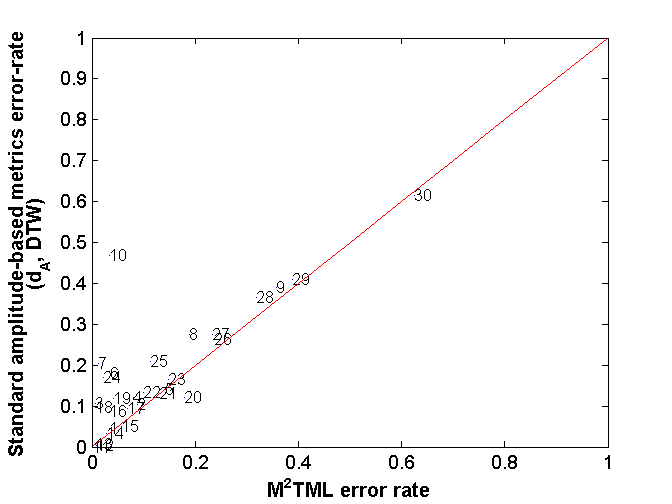
\includegraphics[width = 3in]{Stand_m2tml_2}}
	\subfloat[]{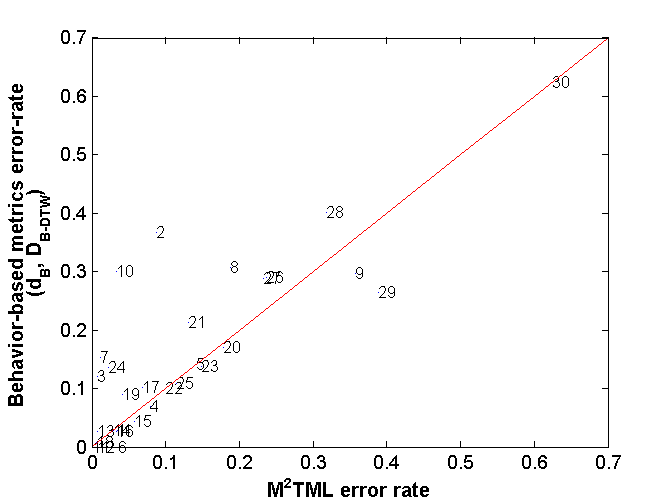
\includegraphics[width = 3in]{behavior_m2tml_2}}\
	\subfloat[]{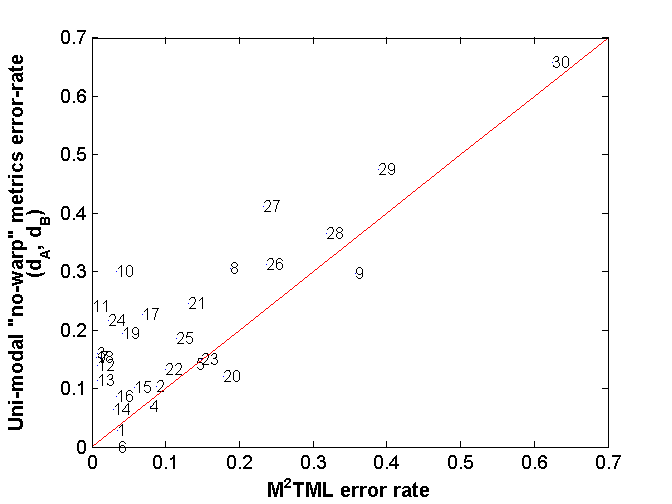
\includegraphics[width = 3in]{no_warp_m2tml_2}}
	\subfloat[]{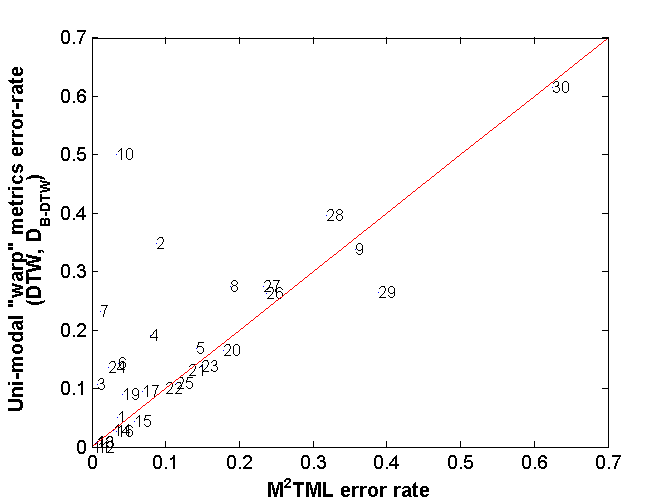
\includegraphics[width = 3in]{Unimod_m2tml_2}} \
	\subfloat[]{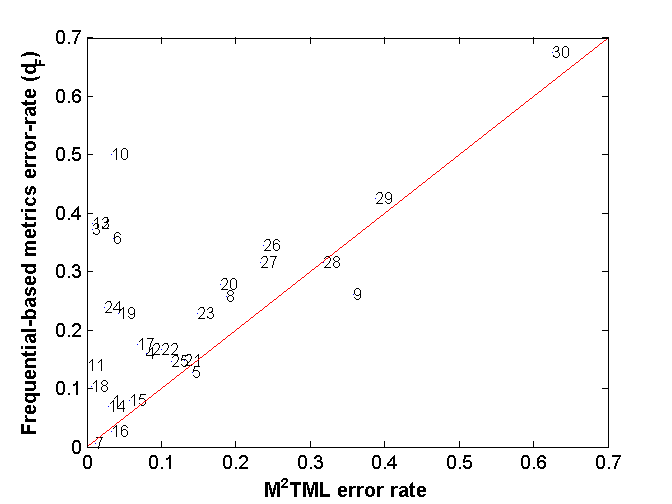
\includegraphics[width = 3in]{freq_m2tml_2}} 	\subfloat[]{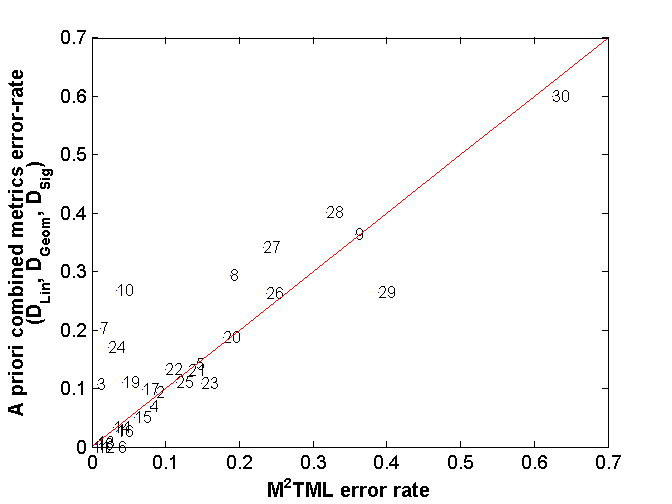
\includegraphics[width = 3in]{apriori_m2tml_2}}\	   
	\caption{(a) Standard amplitude-based (Euclidean distance $d_A$  and {\sc dtw}) vs. {\sc m}$^2${\sc tml} ($D$ and $D_{\mathcal{H}}$) metrics. 
	(b) Behavior-based ($d_B$  and $d_{B-\mbox{\sc dtw}}$) vs. {\sc m}$^2${\sc tml} metrics. 	
	(c) No-warp ($d_A$  and $d_{B}$) vs. {\sc m}$^2${\sc tml} metrics. 
	(d) Warp ({\sc dtw}  and $d_{B-\mbox{\sc dtw}}$) vs. {\sc m}$^2${\sc tml}  metrics. 	
	(e) Frequential-based ($d_F$) vs. {\sc m}$^2${\sc tml} metrics.
	(f) \textit{A priori} ($D_{Lin}$, $D_{Geom}$, $D_{Sig}$) vs. {\sc m}$^2${\sc tml} metrics. 
	}
	\label{fig:error2}
\end{figure}


\subsection{Analysis of the discriminative features}
For the learned metric $D$, thanks to the $L_1$ regularization, the learned {\sc svm} reveals the features that most differentiate pull from push pairs. We recall that the weight for each feature can be analyzed through the weight vector $\textbf{w}$ obtained by learning the {\sc svm} classifier. Table \ref{tab-feature} shows the sparse, muti-modal and multi-scale potential of {\sc m}$^2${\sc tml} approach.  It gives for each dataset, the weights of the top five 'discriminative' features that contribute to the definition of $D$.  For instance,   for FaceFour $D$ reaches an error of 2.3\% by combining, in the order of importance, the behavior $d_{B-\mbox{\sc dtw}}$,  frequential $d_F$ and amplitude {\sc dtw} modalities, at the global ($I^0$) and  local ($I^4$, $I^5$, $I^2$) scales. For Beef, the learned model is very sparse as $D$ involves only the behavior modality based on the segment $I^3$ ($d_B^3$). Note that if we look at only the most discriminative feature (1st column), the {\sc m}$^2${\sc tml} method helps to localize discriminative modality and a specific temporal scale (localization) that could not be easily guessed \textit{a priori} (\textit{e.g.}, Lightning7: behavior modality on the segment $I_6$ ($d_{B-\mbox{\sc dtw}}^6$), OliveOil: frequential modality on the segment $I_5$ ($d_F^5$), TwoLeadECG: behavior modality on the segment $I_4$ ($d_{B-\mbox{\sc dtw}}^4$)). 

\noindent In Fig. \ref{fig:w}, we plot the weights of all features for SonyAIBO, Beef, CincECGtorso and FaceFour cases as an example. It illustrates both the sparsity of the {\sc m}$^2${\sc tml} approach (Beef, CincECGtorso and FaceFour) and the ability of the algorithm to combine all the features into the metric $D$ (SonyAIBO). In particular, the approach is able to either select one single feature (Beef) or combine several selected features (CinCECGTorso, FaceFour). Fig. \ref{fig:temporal_rep} illustrates the temporal locations of the most discriminative features for these datasets. Note that from looking at the temporal representation, it is not easy to determine \textit{a priori} which modality (value, behavior, frequential) and at which temporal scale (localization) is the most discriminative feature to separate the classes.

\noindent In summary, we can emphasize that for almost all datasets, the definition of  $D$ involves no more than five features (the most contributive ones), that assesses not only the model's sparsity but also  the representativeness of the revealed features.
%\todo{Erreur dans la these, pas db-DTW mais dB}
\begin{table}[h!]
	%	\small
	\centering
	\renewcommand{\arraystretch}{1.3}
	\resizebox{1\textwidth}{!}{
		\setlength{\tabcolsep}{1pt}
		\begin{tabular}{| c |  l l l l l |}
			\hline
			Dataset & \multicolumn{5}{c|}{Feature weights  (\%)}  \\ 
			\hline 
			%\vspace{0.1cm}
			ItalyPowerD 		& $d_B^0$ (27.5\%) &$d_F^4$ (17.2\%) &$d_F^1$ (12.3\%) &$d_A^1$ (11.2\%) &$d_B^2$ (9\%)
			\\			
			CinCECGtorso		& $d_F^0$ (38.4\%)&   $d_A^5$ (13.1\%)&   $d_B^4$ (11.5\%)&   $d_F^1$ (11.2\%)&   $d_A^2$ (9.8\%)   
			\\		
			BME 				& $d_{B-\mbox{\sc dtw}}^0$ (75.2\%)&   $d_F^4$ (15.5\%)&   $d_{B-\mbox{\sc dtw}}^2$ (5.8\%)&   $d_{B-\mbox{\sc dtw}}^1$ (1.9\%)&   $d_F^1$ (0.7\%)   
			\\	
			ECG200				& $d_B^0$ (89.6\%)&   $d_B^6$ (2.4\%)&   $d_A^3$ (2.3\%)&   $d_B^1$ (2.2\%)&   $d_B^4$ (2\%)  
			\\		
			SonyAIBOII			& $d_B^3$ (100\%)& -   & - & - &- 		
			\\
			Coffee				& $d_F^4$ (59.4\%) &$d_B^6$ (6.4\%) &$d_B^2$ (5.6\%) &$d_B^3$ (5\%) &$d_F^5$ (4.4\%)
			\\	
			ECG5Days			& $d_B^5$ (44.9\%) &$d_B^6$ (36.3\%) &$d_A^4$ (7.9\%) &$d_F^6$ (7.4\%) &$d_B^4$ (2.7\%)
			\\	
			SonyAIBO			& $d_F^3$ (30.8\%)&   $d_B^6$ (27.3\%)&   $d_B^5$ (5\%)&   $d_A^1$ (4.1\%)&   $d_B^0$ (3.9\%)   
			\\		
			Adiac				& $d_F^0$ (79.2\%)&   $d_B^4$ (13.8\%)&   $d_A^4$ (3.5\%)&   $d_F^5$ (1.7\%)&   $d_B^5$ (1.2\%)   
			\\	
			Beef				& $d_B^3$ (100\%)& - & - &-  & -  
			\\
			Trace 				& {\sc dtw}$^0$ (58.3\%)&   {\sc dtw}$^6$ (6.9\%)&   $d_{B-\mbox{\sc dtw}}^0$ (5.8\%)&   {\sc dtw}$^2$ (5.6\%)&   {\sc dtw}$^5$ (5.5\%) 
			\\			
			CBF 				& $d_F^6$ (18.5\%) &$d_F^3$ (18.5\%) &$d_F^0$ (15.2\%) &{\sc dtw}$^4$ (12.4\%) &$d_F^1$ (9\%)
			\\																				
			CC					& $d_F^0$ (17.1\%) & {\sc dtw}$^3$ (13.2\%) & {\sc dtw}$^2$ (11.4\%) &$d_{B-\mbox{\sc dtw}}^2$ (11\%) &$d_F^1$ (7.1\%)
			\\
			DiatomSizeR 		& $d_F^5$ (100\%) & - & - & -  & - 
			\\			
			Symbols 			& $d_F^6$ (38.2\%) & {\sc dtw}$^0$ (16.1\%) & {\sc dtw}$^1$ (12\%) &$d_F^0$ (6.7\%) &{\sc dtw}$^2$ (4.7\%)	
			\\			
			GunPoint			& $d_{B-\mbox{\sc dtw}}^0$ (41.1\%) &{\sc dtw}$^5$ (14.7\%) &{\sc dtw}$^2$ (9.5\%) & {\sc dtw}$^4$ (6.1\%) & $d_F^4$ (6\%)	
			\\			
			FacesUCR			& $d_F^2$ (21.5\%)&   $d_{B-\mbox{\sc dtw}}^0$ (19.5\%)&   $d_F^4$ (16.7\%)&   {\sc dtw}$^0$ (12.6\%)&   $d_{B-\mbox{\sc dtw}}^2$ (8.6\%)
			\\			
			TwoLeadECG 			& $d_{B-\mbox{\sc dtw}}^4$ (60\%)&   $d_F^1$ (12\%)&   {\sc dtw}$^4$ (11.4\%)&   $d_{B-\mbox{\sc dtw}}^6$ (7.6\%)&   $d_{B-\mbox{\sc dtw}}^1$ (4.2\%)
			\\			
			UMD 				& $d_{B-\mbox{\sc dtw}}^0$ (99.8\%) &$d_{B-\mbox{\sc dtw}}^5$ (0.2\%) & - & - & -
			\\			
			MoteStrain			& $d_{B-\mbox{\sc dtw}}^5$ (93.2\%)&   $d_{B-\mbox{\sc dtw}}^6$ (6.8\%)& -  & - & -
			\\
			Lighting2			& $d_{B-\mbox{\sc dtw}}^0$ (100\%) & {\sc dtw}$^0$ (0\%) & $d_F^0$ (0\%) & {\sc dtw}$^1$ (0\%) & $d_{B-\mbox{\sc dtw}}^1$ (0\%)
			\\			
			OliveOil			& $d_F^5$ (97\%)&   $d_{B-\mbox{\sc dtw}}^2$ (3\%)   & - & - & -
			\\						
			FISH				& $d_{B-\mbox{\sc dtw}}^5$ (17.9\%)&   $d_F^0$ (10.5\%)&   $d_{B-\mbox{\sc dtw}}^6$ (9.9\%)&   $d_{B-\mbox{\sc dtw}}^4$ (8.3\%)&   $d_{B-\mbox{\sc dtw}}^3$ (7.8\%)  
			\\
			FaceFour			& $d_{B-\mbox{\sc dtw}}^4$ (66.7\%) &$d_F^4$ (22.4\%) & $d_{B-\mbox{\sc dtw}}^3$ (5.6\%) &$d_{B-\mbox{\sc dtw}}^1$ (5.3\%) & -
			\\
			SwedishLeaf			& $d_F^0$ (23.9\%) &$d_{B-\mbox{\sc dtw}}^1$ (14.1\%) &$d_{B-\mbox{\sc dtw}}^2$ (10.5\%) &$d_{B-\mbox{\sc dtw}}^6$ (10\%) &$d_{B-\mbox{\sc dtw}}^5$ (6\%)	
			\\
			MedicalImages		& $d_{B-\mbox{\sc dtw}}^1$ (53.3\%)&   $d_F^3$ (12.9\%)&   $d_{B-\mbox{\sc dtw}}^2$ (10.7\%)&   $d_{B-\mbox{\sc dtw}}^3$ (10.1\%)&   $d_{B-\mbox{\sc dtw}}^0$ (3.8\%)   
			\\
			Lighting7			& $d_{B-\mbox{\sc dtw}}^6$ (77.7\%) &$d_F^6$ (20.8\%) &$d_{B-\mbox{\sc dtw}}^5$ (1.5\%) &{\sc dtw}$^3$ (0\%) &{\sc dtw}$^1$ (0\%)		
			\\
			PowerCons			& $d_F^0$ (26.1\%)&   {\sc dtw}$^0$ (20.3\%)&   $d_F^1$ (19.3\%)&   $d_{B-\mbox{\sc dtw}}^0$ (6.1\%)&   $d_F^2$ (5.1\%) 
			\\
			OSULeaf				& $d_{B-\mbox{\sc dtw}}^2$ (84.7\%) &$d_F^6$ (7.7\%) &$d_F^0$ (2.7\%) &$d_F^5$ (1.6\%) & {\sc dtw}$^5$ (1.2\%)
			\\
			InlineSkate			& {\sc dtw}$^2$ (25.7\%) &$d_F^4$ (24.3\%) &$d_F^3$ (16.5\%) &$d_{B-\mbox{\sc dtw}}^2$ (11.2\%) &$d_{B-\mbox{\sc dtw}}^3$ (5.2\%)		 
			\\
			\hline
		\end{tabular}
	}
	\caption{Top 5  multi-modal and multi-scale features involved in  $D$}
	\label{tab-feature}
\end{table}

\begin{figure}[h!]
	\centering
%	\subfloat[SonyAIBO]{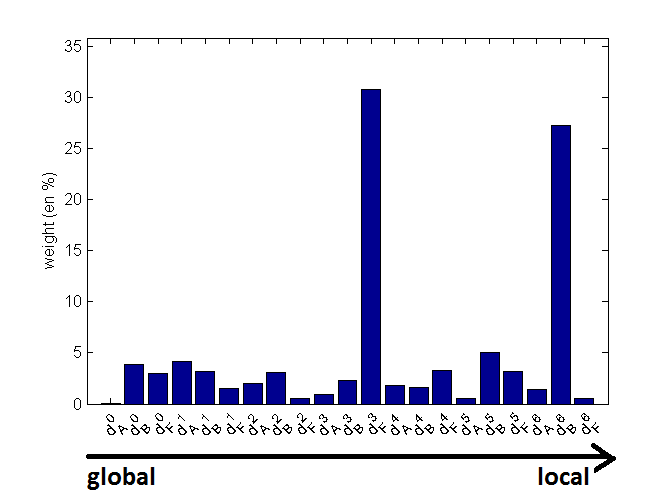
\includegraphics[width = 3in]{SonyAIBO_weight_V2}} \
	\subfloat[SonyAIBO]{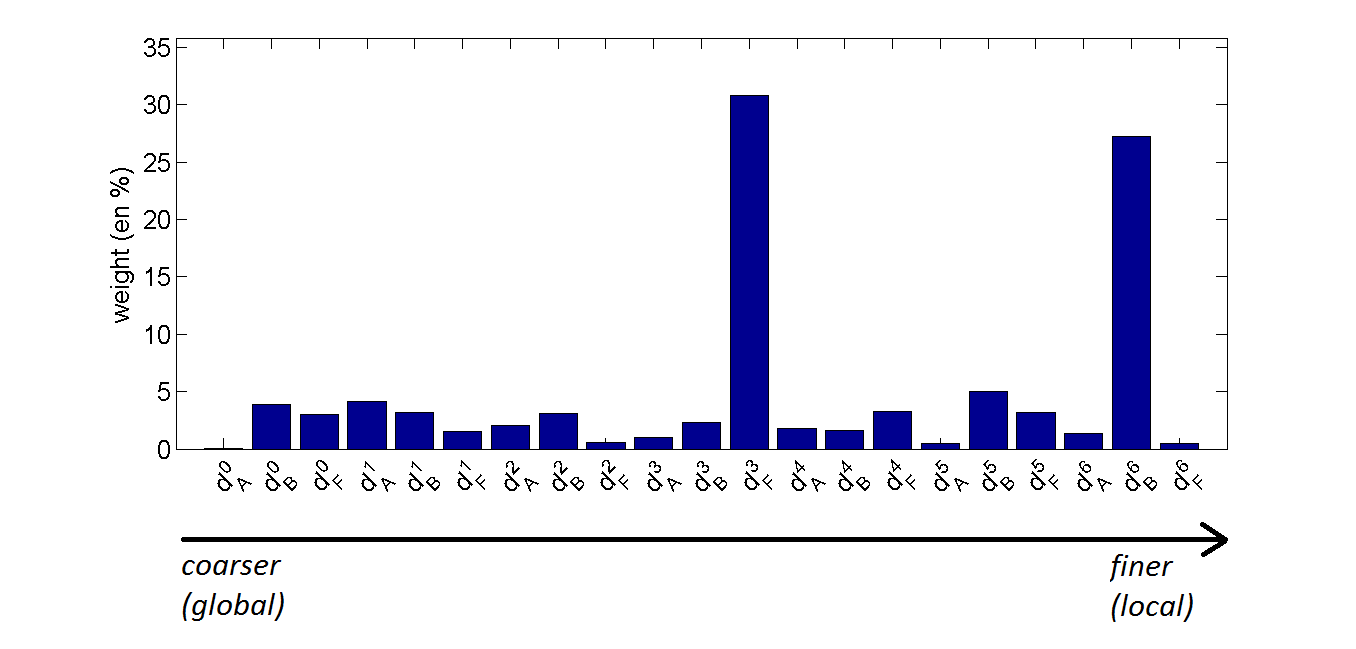
\includegraphics[width = 3.5in]{SonyAIBORobotSurface_NoDelay_bar2}} \
	\subfloat[Beef]{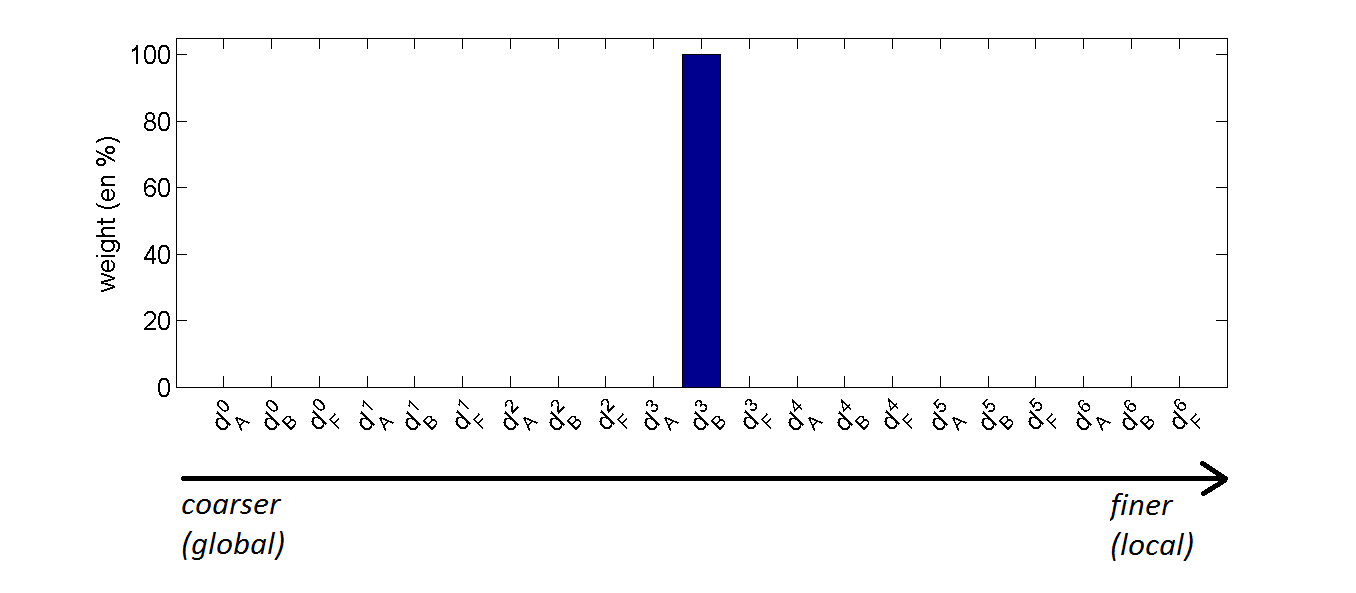
\includegraphics[width = 3.5in]{Beef_NoDelay_bar2}}\    
	\subfloat[CinC ECG torso]{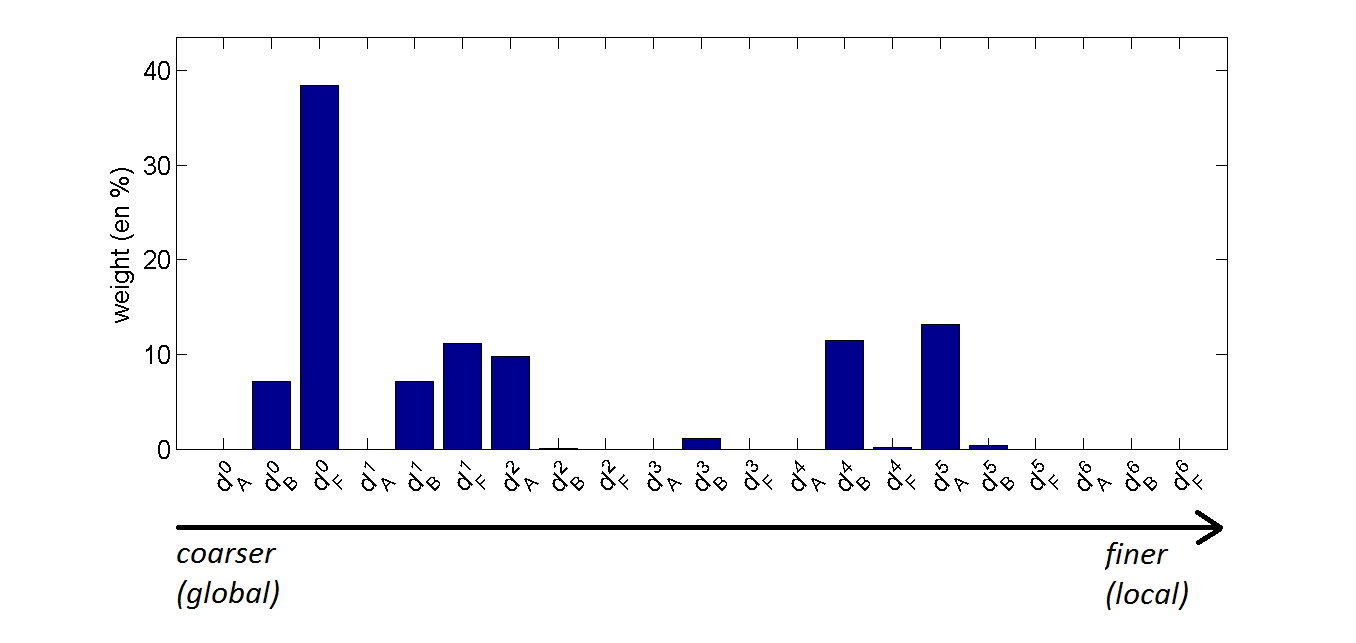
\includegraphics[width = 3.5in]{CinC_ECG_torso_NoDelay_bar2}} \
	\subfloat[FaceFour]{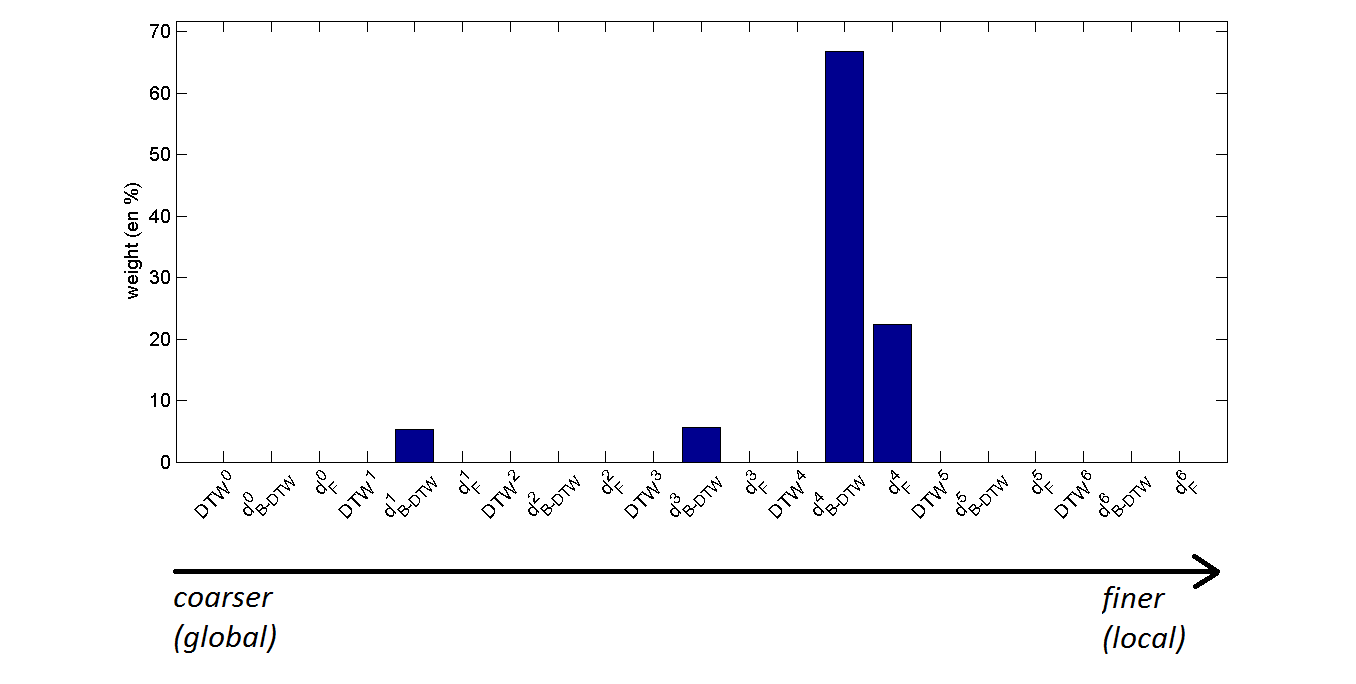
\includegraphics[width = 3.5in]{FaceFour_DTW_bar2}} 
	\caption{{\sc m}$^2${\sc tml} feature weights for 4 datasets.}
	\label{fig:w}
\end{figure}

\begin{figure}[h!]
	\centering
	\subfloat[SonyAIBO]{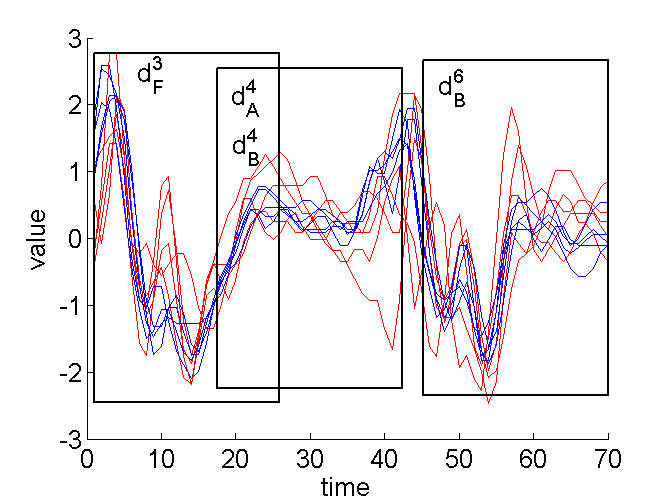
\includegraphics[width = 2.7in]{SonyAIBORobotSurface_NoDelay_TS}} 
	\subfloat[Beef]{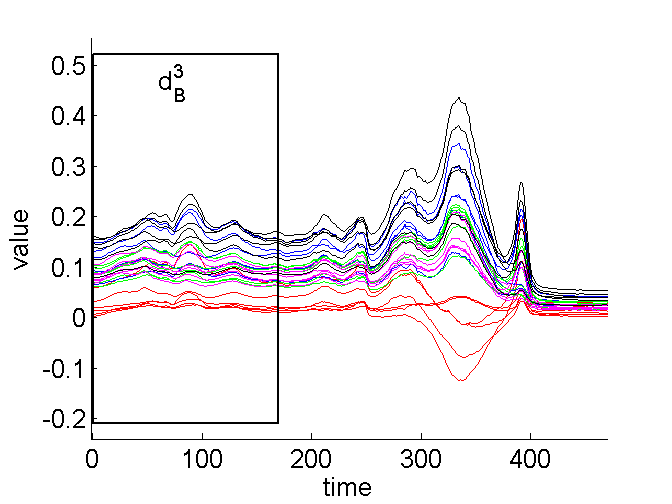
\includegraphics[width = 2.7in]{Beef_NoDelay_TS}} \   
	\subfloat[CinC ECG torso]{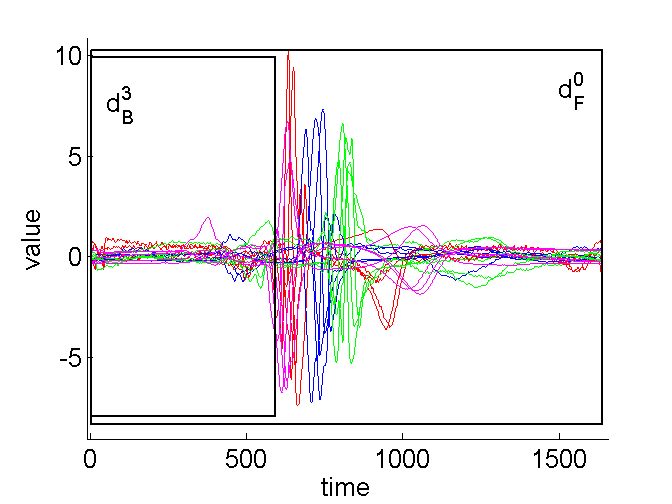
\includegraphics[width = 2.7in]{CinC_ECG_torso_NoDelay_TS}}
	\subfloat[FaceFour]{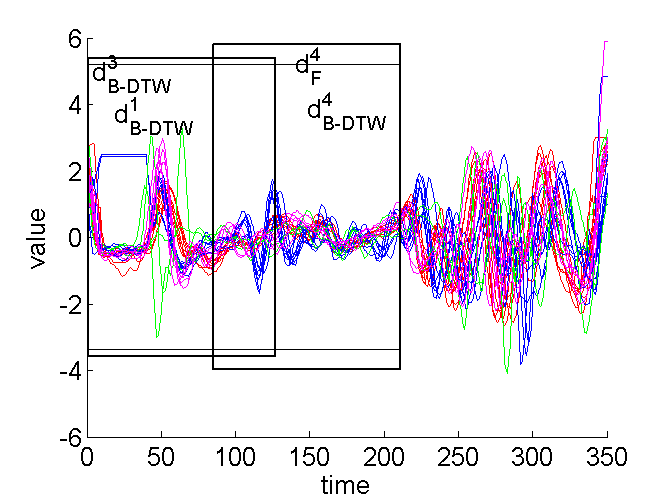
\includegraphics[width = 2.7in]{FaceFour_DTW_TS2}} 
	\caption{Temporal representation of the top {\sc m}$^2${\sc tml} feature weights for 4 datasets.}
	\label{fig:temporal_rep}
\end{figure}


%\begin{figure}[h!]
%	\centering
%	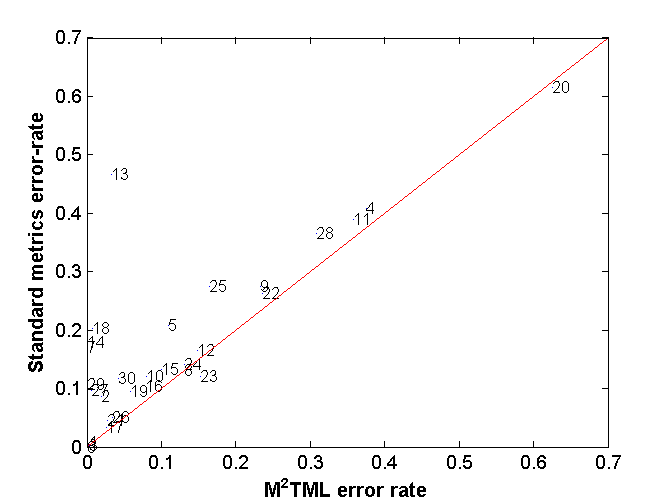
\includegraphics[width=0.6\linewidth]{images/Stand_m2tml}
%	\caption{Standard (Euclidean distance $d_A$  and {\sc dtw}) {\it vs.} {\sc m}$^2${\sc tml} ($D$ and $D_{\mathcal{H}}$) metrics }
%	\label{fig:error1}
%\end{figure}
%\begin{figure}[h!]
%	\centering
%	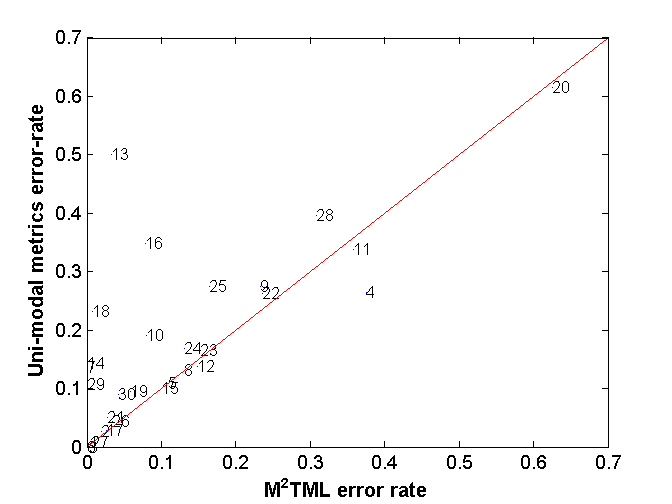
\includegraphics[width=0.6\linewidth]{images/Unimod_m2tml}
%	\caption{Best Uni-modal ({\sc dtw} and $d_{B-\mbox{\sc dtw}}$) {\it vs.} {\sc m}$^2${\sc tml} ($D$  and $D_{\mathcal{H}}$) metrics }
%	\label{fig:error2}
%\end{figure}

\begin{figure}[h!]
	\centering
	\subfloat[FaceFour ($d_{B-\mbox{\sc dtw}}$, stress: 20,1\%)]{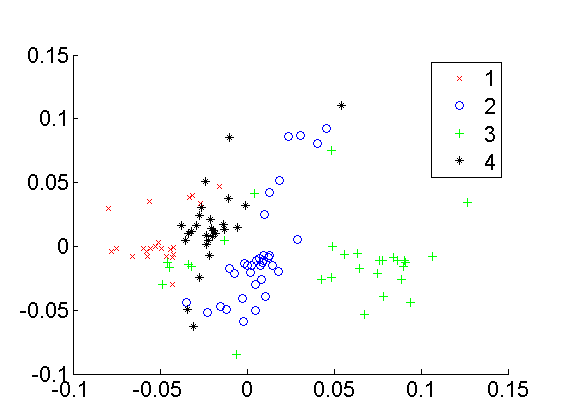
\includegraphics[width = 3in]{FaceFourALL_DTWDB_2}} 
	\subfloat[FaceFour ($D$, stress: 18,9\%)]{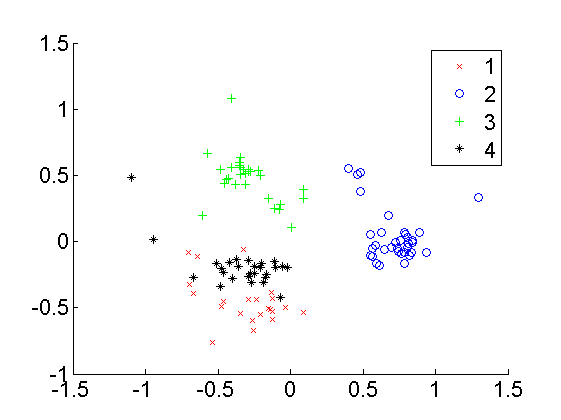
\includegraphics[width = 3in]{FaceFourALL_D_Delay_3}} \  
%	\subfloat[]{\includegraphics[width = 3in]{CinC_ECG_torso_MDS_DA}} 
%	\subfloat[]{\includegraphics[width = 3in]{CinC_ECG_torso_MDS_After}}  
	\caption{{\sc mds} visualization of the $d_{B-\mbox{\sc dtw}}$ (Fig. a) and $D$ (Fig. b) dissimilarities for FaceFour}
	\label{fig:mds}
\end{figure}

\newpage
\subsection{Effect on the neighborhood before and after learning}
In the last part, we compare the global effect of the alternative and {\sc m}$^2${\sc tml} metrics  on the $1$-NN neighborhood distribution and class discrimination. For that, a MultiDimensional Scaling\footnote{Matlab function: mdscale for metrics and non metrics} ({\sc mds}) is used to visualize the distribution of samples according to their pairwise  dissimilarities. Briefly, we recall that {\sc mds} is a method of visualizing the proximity between samples in a dataset (Section \ref{sec:property_metric}). Given an input dissimilarity matrix, we can project the time series on a 2-dimensional plot whose configuration reproduces the best the dissimilarities between the time series. Note that the {\sc mds} representation has no link with the dissimilarity space representation whose dimensions are basic temporal metrics.

For FaceFour, Fig. \ref{fig:mds} shows the first obtained plans and their corresponding stresses, the classes being indicated in different symbols and colors. We can see distinctly the effect of the learned  $D$ that leads to  more compact and more isolated classes with  robust  neighborhoods for 1-NN classification ({\it i.e.}, closer pull pairs and far away push pairs) than  the best alternative metric $d_{B-\mbox{\sc dtw}}$ that shows more overlapping classes and heterogeneous neighborhoods.
%\begin{figure}[h!]
%	\centering
%	% \includegraphics[width=0.6\linewidth]{images/FaceFourALL_DTWDB_1} \hspace{-0.45cm}
%	% \includegraphics[width=0.6\linewidth]{images/FaceFourALL_D_Delay_1}
%	\includegraphics[width=1\linewidth]{FaceFour}
%	\caption{{\sc mds} visualization of the $d_{B-\mbox{\sc dtw}}$ (left) and $D$ (right) dissimilarities for FaceFour data}
%	\label{fig:mds}
%\end{figure} 

\section{Conclusion of the chapter}
%%% Local Variables: 
%%% mode: latex
%%% TeX-master: "../roque-phdthesis"
%%% End: 
% This paper proposes a new Multi-modal and Multi-scale Temporal Metric Learning ({\sc m}$^2${\sc tml}) framework  for large margin time series nearest neighbors classification. 
% For this, time series are embedded  into a  dissimilarity space  where a  function combining several modalities at different temporal scales can be learned,  driven jointly by a pairwise {\sc svm} and nearest neighbors metric learning framework.  Thanks to the 'kernel trick',  the {\sc m}$^2${\sc tml} approach  provides a temporal metric learning solution for linear as well as  non linear contexts. A sparse and interpretable variant of the solution  shows the ability of the learned temporal metric to localize accurately discriminative  modalities as well as their temporal scales.   
The large conducted experiments and the impressive performances obtained  attest the efficiency of the learned {\sc m}$^2${\sc tml} metrics for time series nearest neighbors classification. As discussed, the datasets encompass time series that involve global or local temporal comparison, require or not time warping, with linearly or non linearly separable neighborhoods. \\
Finally, let us underline the merit of the {\sc m}$^2${\sc tml}  solution, that not only leads to equivalent or better performances from the standard metrics (Euclidean distance, Dynamic time warping), but also provides a comprehensive and fine-grained information about  which modalities are mostly discriminant, how they should be combined and precisely at which temporal granularity (localization). 
\part*{Conclusion of Part II}




\chapter*{Conclusion and perspectives}
\addstarredchapter{Conclusion}
\markboth{Conclusion}{Conclusion}
\label{sec:conclusion}

\section*{Conclusion}
In this PhD, we have proposed a framework to learn a combined multi-modal and multi-scale temporal metric (\textsc{m$^2$tml}) for a robust $k$-NN classifier. It is based on a new space representation, the dissimilarity space, where pairs of time series are embedded as vectors described by different basic temporal metrics. A metric combining the basic metrics can be seen as a function of the dissimilarity space, learned by using a large margin optimization process (\textsc{svm}) inspired from the nearest neighbors metric learning framework. The obtained metric satisfies the properties of a dissimilarity, leads to good performances on a large number of public datasets, and gives an interpretable solution that allows to analyze the modalities and scales that are the most discriminant.

Temporal data may be compared based on various characteristics or modalities. They may be compared not only on their amplitudes like static data, but also on other modalities such that their behavior, frequency, etc. Some authors propose to combine several modalities but are either, limited to two modalities or in case of multiple modalities (more than 2), the number of parameters to optimize for the classifier may become time consuming. In general, state of the art approaches compared the time series by involving all observations, restricting the potential of comparison measures (metrics) to capture local differences. Real time series can be also subjected to delays. We believe that all of these considerations (modality, scale, delays) should be taken into consideration in the definition of a metric in order to improve the performance of the classifier.

In the second part of this work, we propose a general formalization of the problem of learning a combined multimodal and multiscale temporal metric (\textsc{m$^2$tml}) for a robust $k$-NN. Based on a pairwise dissimilarity representation of the pairs of time series, the metric learning learning can be reduced to the learning of a linear or non linear function of the dissimilarity space that satisfies the properties of a dissimilarity (positivity, reflexivity, symmetry). Inspired from metric learning work, the problem is formalized as an optimization problem involving a regularization and loss term which aims to pull samples that are expected to be similar and push away samples that should be dissimilar. By considering a linear combination of the basic metrics, changing the regularization term leads the general formalization to a linear and quadratic formalization. The latter allows to extend to the learning of non-linear functions thanks to the "kernel" trick. However, the methods can lead to functions that doesn't meet the properties of a dissimilarity (non-positivity). Secondly, we formulate the problem as a \textsc{svm} problem which aims to separate pull and push samples, then we define a metric that satisfy the required properties. 

The efficiency of the proposed \textsc{svm}-based solution has been tested in the case of classification of univariate time series, on a wide variety of datasets coming from various fields (simulated data, medicine, power consumption, etc.), diverse sizes of training and testing, various number of classes, etc. The \textsc{m$^2$tml} solution achieves not only, either equivalent or better performances compared to the standard global metrics (euclidean distance, dynamic time warping, temporal correlation, Fourier distance), but it also provides a sparse and interpretable solution that allows to give a comprehensive analysis of the most discriminative modalities and their respective temporal granularity that may not be always intuitive \textit{a priori}. 

\section*{Perspectives}
\subsection*{Extension to other modalities, multivariate problems and other type of data}
In this work, we focus on three basic temporal metrics (euclidean distance, temporal correlation, Fourier-based distance). Montero \& Vilar propose in \cite{Montero2014} a review on a wide number of metrics dedicated to time series. For remaining challenging datasets in our experiments, it could be interesting to integrate other basic temporal metrics in our framework to see the obtained results.

\noindent The framework can be easily extend to multivariate problem. For each dimension, we consider the set of multimodal and multiscale description. Then,  we consider the union over the dimensions as our new pairwise dissimilarity description $d_1, \ldots, d_p$. 

\noindent The proposed framework has been tested in the case of time series data but is more general. It can be applied to any other type of data (strings, graphs, images) to learn a combined metric. Deza \& Deza makes a detailed review of metrics for various domains in \cite{Deza2009}.


\subsection*{Multiscale description}
A second improvement is about the multiscale description. Our multiscale approach is based on a binary segmentation using a dichotomy process. Other solutions could be proposed to localize for finely event of interest. For example, in the case of the dataset SonyAIBO, the discriminative temporal location of the signal is known \textit{a priori} (Fig. \ref{fig:SonyAIBO_tmp}). With the actual multiscale description, it is not possible to extract exactly the two red patterns of interest. A solution based on a sliding window of variable lengths could be used to locate precisely these patterns. 

\begin{figure}[h!]
	\centering
	\includegraphics[width=1\linewidth]{SonyAIBO_temp}
	\caption{(a) Two classes of time series from the Sony AIBO accelerometer. (b) The and-shapelets from the walk cycle on carpet. (c) The Sony AIBO Robot.\protect\footnotemark}
	\label{fig:SonyAIBO_tmp}
\end{figure}
\footnotetext{source: \url{http://www.cs.ucr.edu/~eamonn/LogicalShapelet.pdf}}

\subsection*{Learning of local metrics}
Some authors \cite{Weinberger2009a, Wang2012} suggest that in some datasets, global linear metric learning approach are not sufficient to improve the accuracy of $k$-NN classification. However, since the discriminatory power of the input features might vary between different neighborhoods, learning a global metric cannot fit well the distance over the data manifold. To overcome this difficulty, they propose to learn a metric on each neighborhood, referred as local metric learning. \\
Similarly, our \textsc{m$^2$tml} framework could be extended to learn local combined metric for each neighborhood. The objective is to learn for each $n$ set $Pull_i$ and $Push_i$ ($n$ being the number of samples in the training set) a local metric using the same framework than the one we propose in this work. We obtain $n$ local metrics $D_i$. Then, to classify a new sample $\textbf{x}_{test}$, we compute the $n$ metrics $D_i(\textbf{x}_{i,test})$ and classify $\textbf{x}_{test}$ using the $k$ lowest $D_i(\textbf{x}_{i,test})$.


\subsection*{Re-iteration of the initial metric}
Similarly to Large Margin Nearest Neighbors (\textsc{lmnn}) approach proposed by Weinberger \& Saul \cite{Weinberger2009a}, our approach may inherit the same problem of defining the set $Pull_i$ and $Push_i$ according to an initial distance (L2-norm in our work). Other initial distance could have been used. If the initial distance is far away from the optimal solution, the definition of the sets $Pull_i$ and $Push_i$ can impact the convergence to the optimal solution. In same spirit as the multi-pass (\textsc{lmnn}) approach proposed by Weinberger \& Saul, we could re-iterate the learning process. At each step, we re-define the sets $Pull_i$ and $Push_i$ using the distance learned at the previous step. Then, we stop the learning when arriving at convergence (\textit{e.g.}, the sets $Pull_i$ and $Push_i$ doesn't evolve anymore between two steps).

\subsection*{Other proposition to define the combined metric}
\todo[inline]{Proposition de Sylvain}

\subsection*{Extension to regression problems}
For the \textsc{svm}-based solution, in the pairwise dissimilarity space, each vector $\textbf{x}_{ij}$ is labeled $y_{ij}$ by following the rule: if $\textbf{x}_i$ and $\textbf{x}_j$ are similar, the vector $\textbf{x}_{ij}$ is labeled -1; and +1 otherwise. \\
For classification problems, the concept of similarity between samples $\textbf{x}_i$ and $\textbf{x}_j$ is driven by the class label $y_i$ and $y_j$ in the original space:
\begin{equation}
y_{ij} = 
\left\{
\begin{split}
+1 \text{\quad if } y_i = y_j\\ 
-1 \text{\quad if } y_i \neq y_j
\end{split}
\right.
\end{equation}
For regression problems, each sample $\textbf{x}_i$ is assigned to a continuous value $y_i$. Two approaches are possible to define the similarity concept. The first one discretizes the continuous space of values of the labels $y_i$ to create classes. One possible discretization bins the label $y_i$ into $Q$ intervals as illustrated in Fig. \ref{fig:Discretize_binning}. Each interval becomes a class which associated value can be set for example as the mean or median value of the interval. Then, the classification framework is used to define the pairwise label $y_{ij}$.

\begin{figure}[h!]
	\centering
	\includegraphics[width=0.6\linewidth]{images/Discretize_binning}
	\caption{Example of discretization by binning a continuous label $y$ into $Q=4$ equal-length intervals. Each interval is associated to a unique class label. In this example, the class label for each interval is equal to the mean in each interval.}
	\label{fig:Discretize_binning}
\end{figure}

\noindent This approach may leads to border effects between the classes. For instance, two samples $\textbf{x}_i$ and $\textbf{x}_j$ that are close to a frontier and that are on different sides of the border will be considered as different, as illustrated in Fig \ref{fig:Discretize_binning_border_effect}. Moreover, a new sample $\textbf{x}_j$ will have its labels $y_j$ assigned to a class and not a real continuous value. 

\begin{figure}[h!]
	\centering
	\includegraphics[width=0.42\linewidth]{images/Discretize_binning_border_effect}
	\caption{Border effect problems. In this example, $\textbf{x}_2$ and $\textbf{x}_3$ have closer value labels $y_2$ and $y_3$ than $\textbf{x}_3$ and $\textbf{x}_4$. However, with the discretization $\textbf{x}_2$ and $\textbf{x}_3$ don't belong to the same class and thus are consider as not similar.}
	\label{fig:Discretize_binning_border_effect}
\end{figure}

\noindent The second approach considers the continuous value of $y_i$, computes a $L_1$-norm between the labels $|y_i-y_j|$ and compare this value to a threshold $\epsilon$. Geometrically, a tube of size $\epsilon$ around each value of $y_i$ is built. Two samples $\textbf{x}_i$ and  $\textbf{x}_j$ are considered as similar if the absolute difference between their labels $|y_i-y_j|$ is lower than $\epsilon$ (Fig. \ref{fig:pairwise_label_tube}):
\begin{equation}
y_{ij} = 
\left\{
\begin{split}
\begin{aligned}
-1 & \text{\quad if } |y_i-y_j| \leq \epsilon \\ 
+1 & \text{\quad otherwise }
\end{aligned} 
\end{split}
\right.
\end{equation}

\begin{figure}[h!]
	\centering
	\includegraphics[width=0.65\linewidth]{images/pairwise_label_tube}
	\caption{Example of pairwise label definition using an $\epsilon$-tube (red lines) around the time series $\textbf{x}_i$ (circled in blue). For, time series $\textbf{x}_j$ that falls into the tube, the pairwise label is $y_{ij} = -1$ (similar) and outside of the tube, $y_{ij} = +1$ (not similar).}
	\label{fig:pairwise_label_tube}
\end{figure}


\subsection*{Using the learned combined metric in other algorithms}




\begin{itemize}
%	\item Bilan des apports de la thèse.
%		\begin{itemize}
%			\item \textbf{Objectif}: Dans cette thèse, nous nous sommes intéressés à l'apprentissage de métriques combinées multi-modal et multi-échelle en vue d'une classification kNN robuste.
%			\item \textbf{Uni-modal}: Les données temporelles, contrairement aux données statiques, peuvent être comparés non seulement sur la base de modalités comme les valeurs mais aussi au moins, sans être exhaustifs sur la base de modalités temporelles comme la forme ou la fréquence. De manière classique, la comparaison de séries se fait sur la base d'une modalité à l'échelle globale qui définit les mesures de distance habituellement utilisées (distance euclidienne, corrélation temporelle, distance à base Fourier, etc.).
%			\item \textbf{Multi-modal}: Afin de tenir compte de plusieurs modalités au sein d'une même métrique, certains auteurs ont proposés de combinés plusieurs modalités via des fonctions de combinaisons. Elles sont en général limités à 2 modalités et sont définis sans considération du classifieur. La recherche des meilleurs paramètres peut devenir lourd computationnelement en augmentant le nombre de métriques impliqués dans la combinaison.
%			\item \textbf{Multi-échelle}: Ce travail a mis en évidence l'importance de comparer les séries temporelles à différentes échelles temporelles. Les modalités et métriques cités précédemment peuvent être adaptées afin de comparer les séries, non seulement sur la base de l'échelle globale (impliquant l'ensemble des éléments de la série temporelle) mais aussi à une échelle plus localisées (impliquant une partie des éléments de la séries temporelles).
%			\item \textbf{Metric Learning}: Afin d'améliorer les performances d'un classifieur kNN, certains travaux dans la littérature se sont intéressés à l'apprentissage de la métrique en vue d'une classification robuste kNN. Ces approches reposent en général sur l'apprentissage d'une distance de Mahalanobis dans un cadre linéaire ou non-linéaire. Certains parrallèles avec les SVM ont aussi été étudiés. Les travaux sont nombreux pour les données statiques, moins nombreux pour les données structurées, et en particulier encore dans ses début pour les séries temporelles.
%			\item \textbf{Formalisation}: La seconde partie de ce travail a abouti à la formalisation du problème d'apprentissage métriques combinées multi-modal et multi-échelle en vue d'une classification kNN robuste.
%			\item \textbf{Espace des paires}: Le calcul d'une métrique impliquant toujours deux éléments, nous avons proposé de représenter les paires de séries temporelles dans un espace de dissimilarités où chaque dimension est une métrique temporelle de base (i.e., une modalité à une échelle temporelle). L'apprentissage d'une métrique combinée de plusieurs métriques temporelle de base se ramène alors à l'apprentissage d'une fonction dans l'espace de dissimilarités qui vérifie au moins les propriétés d'une dissimilarité (positivité, reflexivité, symétrie). Rappelons que l'interprétation de proximité dans cet espace sur la proximité des séries dans l'espace d'origine doit être fait avec prudence.
%			\item \textbf{m2tml optimisation}: le problème d'apprentissage de la métrique combinées peut être de manière général ramené à un problème d'apprentissage de métrique. Il est formalisé sous la forme d'un problème d'optimisation impliquant 3 termes: 1) un terme de régularisation dont le but est de rapprocher les paires pull (similaires). 2) un terme loss dont le but est d'éloigner les paires push (dissimilaires). 3) des contraintes liés aux paires dissimilaires. Plusieurs stratégies pour construire les ensembles pull et push ont été proposés. La solution retenue est celle des mNN+ vs mNN-. Nous pensons qu'en élargissant en apprentissage le voisinage au m plus proche permettra de mieux généraliser la métrique lors du test.
%			\item \textbf{Les différentes formalisations}: Depuis le problème général, nous avons proposé 3 formalisations impliquant différentes régularisations ou frameworks: linéaire, quadratic, basé svm. Dans la formalisation linéaire, le terme de régularisation est linéaire et la métrique combinée est une combinaison linéaire des métriques de bases, vérifiant les propriétés d'une dissimilarité. Dans la formalisation quadratique, le terme de régularisation est quadratique. Similairement au développement svm, le problème peut être transformé sous une forme n'impliquant que des produits scalaires, permettant d'étendre l'apprentissage de la métrique combinée à des combinaisons à la fois linéaire comme non-linéaire via le kernel trick. La métrique apprise ne vérifie pas cependant les propriétés d'une dissimilarité (non-positive). 
%			\item \textbf{Solution basée svm}: Dans le framework basé svm, la fonction de distance n'est pas connue a priori. Le but est de construire un classifieur svm qui permet de séparer les ensembles pull et push. Sur la base de la solution obtenue du classifieur, une métrique est bâtie qui respecte les propriétés d'une métrique. En particulier, on souligne 2 éléments importants impliqués dans la métrique: la norme du projeté, la distance à la marge du projeté. La norme du projeté d'une paire permet de mesurer la proximité entre les séries temporelles impliquées dans la paire, d'après les features retenus pour séparer les classes pull et push. Afin d'assurer que la norme des paires push soit inférieurs à celles des paires pull, la distance du projeté à la marge nous permet de déterminer l'appartenance d'une paire à l'ensemble pull ou push. Le terme push est donné par une transformation exponentielle de la distance à la marge du projeté contrôlé par un paramètre qui mesure la force du terme push en fonction de la configuration des données. Grâce au framework svm, la méthode peut être naturellement étendu pour apprendre des fonctions non-linéaires.
%			\item \textbf{Pre-processing lié au svm}: La solution svm retenue nous amène à des éléments de pré-processing nécessaire: normalisation de l'espace des dissimilarités, normalisation des voisinages. 
%			\item \textbf{Expérimentation}: L’efficacité de la méthode proposée m2tml a été vérifiée dans un vaste nombre de données publiques dans le cadre d'une classification 1NN de séries temporelles univariées. Les données considérées étaient de domaines divers, de nombres de classes divers, avec des tailles de séries courtes et longues et un nombre divers de séries en apprentissage. Certaines de ces bases obtiennent des scores concluant avec les métriques valeurs classiques (euclidienne, dtw) et d'autres sont encore ouverts à des améliorations. La méthode proposées m2tml permet d'obtenir soit des scores équivalents aux métriques classiques globales, soit d'améliorer les résultats de la classification. Comparativement aux combinaisons a priori, la méthode atteint des performances similaires mais permet d'ajouter des métriques sans devoir ajouter de nouveaux paramètres à optimiser. Soulignons l'avantage supplémentaire de la méthode à interpréter les résultats obtenus: elle permet de localiser les modalités et localisations temporelles d'intérêt par apprentissage qui permet de purifier les voisinages. Ainsi, lorsque dans le cadre d'une utilisation industrielle, en l'absence de connaissance a priori sur les séries, la méthode permet de comprendre ce qui permet de discriminer au mieux les séries afin d'avoir des voisinages purifiées.
%		\end{itemize}
	\item Perspectives
	\begin{itemize}
		\item \textbf{Extension à d'autres modalités}: Le travail effectué s'est intéressé à 3 types de distance (distance euclidienne, corrélation temporelle, distance à base Fourier). Il existe cependant d'autres mesures de distance pour les séries temporelles qu'il serait intéressant d'étudier (wavelets, MFCC, etc.) (cf article).
		\item \textbf{Découpage multi-échelle}: Dans ce travail, nous avons proposé de découper les séries temporelles avec une architecture dichtomique mais d'autres solutions pourraient être proposées: par exemple une fenêtre glissage qui permettrait de localiser plus finement les évènements d'intérêt (prendre l'exemple de SonyAIBO comme le suggère Sylvain).
		\item \textbf{Multi-pass learning}: le framework proposé souffre du même inconvénient que celui de Weinberger. La distance initiale est une norme 2 dans l'espace des paires. Elle permet de définir les voisinages pour la construction des ensembles pull et push qui reste fixe pendant le processus d'optimisation. Une autre solution serait de ré-itérer la distance apprise pour re-définir les ensembles pull et push et ré-apprendre de manière ittérative la métrique jusqu'à convergence.
		\item \textbf{Autre proposition pour D}: La proposition de définition de la métrique $D$ pourrait être élargie. Par exemple, on pourrait penser à une solution qui permet d'élargir à des lambdas négatifs. Inconvénient: avec un lambda négatif, la métrique aurait un effet pull et non push, qui risque de binariser la métrique en incluant des distances très proches de 0 pour les plus proches voisins. Or dans une classification kNN, la distance des plus proches voisins nous permet de faire la classification. En ramenant les distances des plus proches voisins, proches de 0, on a un risque de moins bien discriminé.
		\item \textbf{Extension au multivarié}: on pourrait facilement étendre le framework pour des séries temporelles multivariées. Pour chaque dimension de la série multivariée, on calcule les métriques de bases de chaque échelle qui deviennent de nouvelles dimensions basiques pour notre algorithme.
		\item \textbf{Extension à la régression}: Le travail pourrait être étendu à des problèmes de régression. Le seul changement qui est impliqué est la définition du label $y_{ij}$ lorsque le label $y_i$ est une valeur continue et non une classe (cf la proposition).
		\item \textbf{Apprentissage locale de la métrique}: Dans le cadre du metric learning, des auteurs se sont intéressés à l'apprentissage de métrique localisés et non globales. On pourrait penser apprendre une métrique par localité (voisinnage) et combinée l'ensemble des métriques locales en une métrique globale.
		\item \textbf{Utilisation de la distance apprise dans d'autres algorithmes}: Dans l'industrie, il est souvent important d'avoir un modèle interprétable. Des algorithmes comme les Arbres de décision apporte une représentation visuelle qui permet de comprendre aisément le modèle appris. Des travaux sur les arbres temporelles ont été effectués dans la littérature (cité papier ahlame) utilisant les métriques classiques (euclidienne, corrélation). On pourrait s'inspirer de ces travaux pour construire un arbre avec la métrique apprise par m2tml.
		
		
	\end{itemize}
\end{itemize}



% This paper proposes a new Multi-modal and Multi-scale Temporal Metric Learning ({\sc m}$^2${\sc tml}) framework  for large margin time series nearest neighbors classification. 
% For this, time series are  embedded  into a  dissimilarity space  where a  function combining several modalities at different temporal scales can be learned,  driven jointly by a pairwise {\sc svm} and nearest neighbors metric learning framework.  Thanks to the 'kernel trick',  the {\sc m}$^2${\sc tml} approach  provides a temporal metric learning solution for linear as well as  non linear contexts. A sparse and interpretable variant of the solution  shows the ability of the learned temporal metric to localize accurately discriminative  modalities as well as their temporal scales.   The large conducted experiments  and the impressive performances obtained  attest the efficiency of the   learned {\sc m}$^2${\sc tml} metrics for time series nearest neighbors classification. Finally, let us underline the merit of the  {\sc m}$^2${\sc tml}  solution, that not only leads to better performances, but also provides a comprehensive and fine-grained information about  which modalities are mostly discriminant, how they should be combined and precisely at which temporal granularity. 

%%% Local Variables: 
%%% mode: latex
%%% TeX-master: "../roque-phdthesis"
%%% End: 


%%%%%%%%%%%%%%%%%%%%%%%%%%%
%%% Appendices are included here %%%
%%%%%%%%%%%%%%%%%%%%%%%%%%%
\appendix
\chapter{Detailed presentation of the datasets}
\label{chap:publications}




%%% Local Variables: 
%%% mode: latex
%%% TeX-master: "../roque-phdthesis"
%%% End: 

\chapter{Solver library}
\label{chap:publications}




%%% Local Variables: 
%%% mode: latex
%%% TeX-master: "../roque-phdthesis"
%%% End: 

\chapter{SVM library}
\label{chap:publications}




%%% Local Variables: 
%%% mode: latex
%%% TeX-master: "../roque-phdthesis"
%%% End: 


% Build the references list
% Bibtex
% \bibliographystyle{alpha}
% \bibliography{references.bib}



% BibLatex
\printbibliography
\addstarredchapter{Bibliographie}
\markboth{Bibliographie}{Bibliographie}

% Include the abstract
\cleardoublepage
\chapter*{}
\thispagestyle{empty}
%\begin{vcenterpage}
\noindent\rule[2pt]{\textwidth}{0.5pt}
\\
{\large\textbf{Résumé ---}}
    La définition d'une métrique entre des séries temporelles est un élément important pour de nombreuses tâches en analyse ou en fouille de données, tel que le clustering, la classification ou la prédiction. Les séries temporelles présentent naturellement différentes caractéristiques, que nous appelons modalités, sur lesquelles elles peuvent être comparées, comme leurs valeurs, leurs formes ou leurs contenus fréquentielles. Ces caractéristiques peuvent être exprimées avec des délais variables et à différentes granularités ou localisations temporelles \textemdash exprimées globalement ou localement. Combiner plusieurs modalités à plusieurs échelles pour apprendre une métrique adaptée est un challenge clé pour de nombreuses applications réelles impliquant des données temporelles. Cette thèse propose une approche pour l'Apprentissage d'une Métrique Multi-modal et Multi-scale ({\sc m}$^2${\sc tml}) en vue d'une classification robuste par plus proches voisins. La solution est basée sur la projection des paires de séries temporelles dans un espace de dissimilarités, dans lequel un processus d'optimisation à vaste marge est opéré pour apprendre la métrique. La solution {\sc m}$^2${\sc tml} est proposée à la fois dans le contexte linéaire et non-linéaire, et est étudiée pour différents types de régularisation. Une variante parcimonieuse et interprétable de la solution montre le potentiel de la métrique temporelle apprise à pouvoir localiser finement les modalités discriminantes, ainsi que leurs échelles temporelles en vue de la tâche d'analyse considérée. L'approche est testée sur un vaste nombre de 30 bases de données publiques et challenging, couvrant des images, traces, données {\sc ecg}, qui sont linéairement ou non-linéairement séparables. Les expériences montrent l'efficacité et le potentiel de la méthode {\sc m}$^2${\sc tml} pour la classification de séries temporelles par plus proches voisins.
%\\
%\\
%{\large\textbf{Mots clés :}}
%    Série temporelle, Apprentissage de métrique, $k$-NN, SVM, classification.
\\
\noindent\rule[2pt]{\textwidth}{0.5pt}
%\vspace{0.5cm}
%\vspace{0.1cm}



\newpage
\thispagestyle{empty}

\begin{vcenterpage}
\noindent\rule[2pt]{\textwidth}{0.5pt}
%\begin{center}
%{\large\textbf{Title in english\\}}
%\end{center}
{\large\textbf{Summary ---}}
    The definition of a metric between time series is inherent to several data analysis and mining tasks, including clustering, classification or forecasting. Time series data present naturally several characteristics, called modalities, covering their amplitude, behavior or frequential spectrum, that may be expressed with varying delays and at different temporal granularity and localization \textemdash exhibited globally or locally.  Combining several modalities at multiple temporal scales to learn a holistic metric is a key challenge for many real temporal data applications.  This PhD proposes a Multi-modal and Multi-scale Temporal Metric Learning ({\sc m}$^2${\sc tml}) approach for robust time series nearest neighbors classification. The solution is based on the embedding of pairs of time series into a pairwise dissimilarity space, in which a large margin optimization process is performed to learn the metric. The {\sc m}$^2${\sc tml}  solution is proposed for  both linear and non linear contexts, and is studied for different regularizers. A sparse and interpretable variant of the solution  shows the ability of the learned temporal metric to localize accurately discriminative  modalities as well as their temporal scales. 
    A wide range of 30 public and challenging datasets, encompassing images, traces and {\sc ecg} data, that are  linearly or non linearly separable, are used to show the efficiency and the potential of  {\sc m}$^2${\sc tml} for time series nearest neighbors classification.
%\\
%\\
%{\large\textbf{Keywords:}}
%    Time series, Metric Learning, $k$-NN, SVM, classification.
\\
\noindent\rule[2pt]{\textwidth}{0.5pt}
\begin{center}
	Schneider Electric	\\
	Université Grenoble Alpes, LIG\\
	Université Grenoble Alpes, GIPSA-Lab \\
\end{center}
\end{vcenterpage}

%%% Local Variables: 
%%% mode: latex
%%% TeX-master: "../roque-phdthesis"
%%% End: 


\end{document}


%%%%%%%%%%%%%%%%%%%%%%%%%%%%%%%%%%%%%%%%%%%%%%%%%%%%%%%%%%%%%%%%%%%%%%%%%%%%%%
%%%%%%%%%%%%%%%%%%%%%%%%%%%%%%%%%%%%%%%%%%%%%%%%%%%%%%%%%%%%%%%%%%%%%%%%%%%%%%
% Extra


% Exemple références
Lorem ipsum dolor sit amet, consectetur adipiscing elit \cite{Roque2012,Roque2012b,Roque2012c,Roque2012d}. Sed non risus \cite{Bello1963}. 

% Exemple figure
amet (fig. \ref{fig:une-image}).
\begin{figure}[htp]
	\centering
	\tikzstyle{block} = [draw, fill=blue!20, rectangle, minimum height=3em, minimum width=6em, text width=6em,text centered]
\begin{tikzpicture}[auto, node distance=3.5cm,>=latex']
\shorthandoff{:} % Evite le bug de compilation avec tikz
    % Longueurs et espacement
    \def\longabove{0.2cm}
    \def\espacement{4cm}

    % Définition des blocs
    \node [block, node distance=\espacement] (codeur) {Codeur};
    \node [block, right of=codeur, node distance=\espacement] (cbs) {Conversion bits/symboles};
    \node [block, right of=cbs, node distance=\espacement] (modulateur) {Modulateur};
 
    % Définition des liens
    \draw [<-] (codeur) -- ++(-2,0) node[left] {$\{b_n\}$};
    \draw [->] (codeur) -- node[above=\longabove] {$\{d_n\}$} (cbs);
    \draw [->] (cbs) -- node[above=\longabove] {$\{c_k\}$} (modulateur);
    \draw [->] (modulateur) -- ++(2,0) node[right] {$s(t)$};
\end{tikzpicture}

	\caption{Exemple de diagramme TikZ.}
	\label{fig:une-image}
\end{figure}


% Exemple tableau
Curabitur eu amet (tab. \ref{tab:un-tableau}).
\begin{table}[ht]
	\begin{center}
		\begin{tabular}{|c|c|c|c|c|}
			\hline
			& $h(t,\tau)$ & $S_{\OP{H}}^{(\alpha)} (f,\tau)$ & $L_{\OP{H}}^{(\alpha)} (\nu,t)$ & $H^{(\alpha)}(f,\nu)$ \\
			\hline
			LTI & $q(\tau)$ & $q(\tau) \delta(f)$ & $Q(\nu)$ & $Q(\nu) \delta(\nu-f)$ \\
			\hline
			LFI & $m(t) \delta(\tau)$ & $M(f) \delta(\tau)$ & $m(t)$ & $M(f)$\\
			\hline
			identité & $\delta(t)$ & $\delta(f)\delta(\tau)$ & $1$ & $\delta(\nu-f)$\\
			\hline
		\end{tabular}
		\caption{Exemple de tableau.}
		\label{tab:un-tableau}
	\end{center}
\end{table}

% Exemple 2 figure
amet (fig. \ref{fig:une-autre-image}).

\begin{figure}[htp]
	\centering
	\includegraphics[width=4cm]{images/bitmap_image}
	\caption{Exemple d'image au format JPG.}
	\label{fig:une-autre-image}
\end{figure}

% Exemple figure
\textbf{\begin{figure}[htp!]
		\centering
		\setlength\figureheight{7cm}
		\setlength\figurewidth{9cm}
		% This file was created by matlab2tikz v0.2.2.
% Copyright (c) 2008--2012, Nico Schlömer <nico.schloemer@gmail.com>
% All rights reserved.
% 
% 
% 

% defining custom colors
\definecolor{mycolor1}{rgb}{0,0.75,0.75}

\begin{tikzpicture}

\begin{axis}[%
view={0}{90},
width=\figurewidth,
height=\figureheight,
scale only axis,
xmin=2, xmax=4.5,
xlabel={$\eta$},
xmajorgrids,
ymin=0.5, ymax=1,
ylabel={$d_{\text{min}}^2$},
ymajorgrids,
legend cell align=left,
legend style={align=left}]
\addplot [
color=black,
dashed,
mark=asterisk,
mark options={solid}
]
coordinates{
 (2,1)(2.1,1)(2.2,1)(2.3,1)(2.4,1)(2.5,1)(2.6,0.937749781479547)(2.7,0.890900393128398)(2.8,0.864988513955105)(2.9,0.827013168393703)(3,0.811347612650328)(3.1,0.792559278041243)(3.2,0.765840563467819)(3.3,0.749680961469385)(3.4,0.741947149227874)(3.5,0.740609493518419)(3.6,0.732128087463441)(3.7,0.717775843626632)(3.8,0.699687461812158)(3.9,0.685018622769455)(4,0.673439611642851)(4.1,0.664624248264608)(4.2,0.658255928882634)(4.3,0.641702335270489)(4.4,0.608326504614558)(4.5,0.580489221369454) 
};
\addlegendentry{$\alpha\text{ =  0\%}$};

\addplot [
color=black,
dashed,
mark=x,
mark options={solid}
]
coordinates{
 (2,1)(2.1,1)(2.2,1)(2.3,1)(2.4,0.958561324724996)(2.5,0.900812804739278)(2.6,0.859608621629443)(2.7,0.828484932127753)(2.8,0.812298837741994)(2.9,0.778916291864501)(3,0.758500630955482)(3.1,0.748375165853317)(3.2,0.745960208532468)(3.3,0.738441167434538)(3.4,0.715506361296671)(3.5,0.696927131434508)(3.6,0.682276848692725)(3.7,0.671128156410174)(3.8,0.663062783265717)(3.9,0.657680299791254)(4,0.621142740976429)(4.1,0.589786339121755)(4.2,0.564530571776849)(4.3,0.54483432747474)(4.4,0.53008799514765)(4.5,0.519641830384595) 
};
\addlegendentry{$\alpha\text{ = 10\%}$};

\addplot [
color=black,
dashed,
mark=triangle,
mark options={solid}
]
coordinates{
 (2,1)(2.1,1)(2.2,1)(2.3,0.966145915091813)(2.4,0.907589260275562)(2.5,0.862273165052718)(2.6,0.833762738286283)(2.7,0.797262289343802)(2.8,0.774689700869446)(2.9,0.763077871790574)(3,0.759584455148894)(3.1,0.735410358863577)(3.2,0.713220246811223)(3.3,0.695713299974315)(3.4,0.682371019886023)(3.5,0.672682085917092)(3.6,0.6661550402729)(3.7,0.644666127799479)(3.8,0.610083129739041)(3.9,0.582172698611821)(4,0.560333265725228)(4.1,0.543883933286703)(4.2,0.532098369213191)(4.3,0.524242326405)(4.4,0.519608701974017)(4.5,0.517545187250875) 
};
\addlegendentry{$\alpha\text{ = 20\%}$};

\addplot [
color=black,
dashed,
mark=triangle,
mark options={solid,,rotate=180}
]
coordinates{
 (2,1)(2.1,1)(2.2,0.995488894312993)(2.3,0.930050749246739)(2.4,0.882604857341179)(2.5,0.840148695151764)(2.6,0.807621264874927)(2.7,0.787889977099099)(2.8,0.777972678915356)(2.9,0.750463202108443)(3,0.726620292578349)(3.1,0.707917379352703)(3.2,0.693763185722015)(3.3,0.683575144048861)(3.4,0.676795290182409)(3.5,0.663350261880571)(3.6,0.627666127013326)(3.7,0.598755039468926)(3.8,0.575986310488554)(3.9,0.558651995817327)(4,0.546003746104731)(4.1,0.537291509323841)(4.2,0.531798375059385)(4.3,0.528867181690889)(4.4,0.527917002741411)(4.5,0.528450017604181) 
};
\addlegendentry{$\alpha\text{ = 30\%}$};

\addplot [
color=black,
dashed,
mark=o,
mark options={solid}
]
coordinates{
 (2,1)(2.1,1)(2.2,1)(2.3,1)(2.4,1)(2.5,0.995096871086856)(2.6,0.937749790013923)(2.7,0.890900391028178)(2.8,0.864988509535523)(2.9,0.827013167946275)(3,0.811347609462027)(3.1,0.79255927917077)(3.2,0.765840564829299)(3.3,0.749680963181722)(3.4,0.741947149533667)(3.5,0.740609492450166)(3.6,0.732128080624777)(3.7,0.71777584554089)(3.8,0.699687463368726)(3.9,0.681193180471954)(4,0.640212533267028)(4.1,0.617585040920557)(4.2,0.608519007405809)(4.3,0.608298095410932)(4.4,0.608326494076335)(4.5,0.580489212682311) 
};
\addlegendentry{Mazo};

\end{axis}
\end{tikzpicture}%
		\caption{Exemple de courbe TikZ.}
		\label{fig:courbe-tikz}
	\end{figure}}


% Exemple équation
\begin{align}
H_{m,n,p,q} &= \DPR{\rproto_{p,q}}{\OP{H} \tproto_{m,n}}\\
&= \iint\limits_{\SET{R}^2} S_{\OP{H}}(f,\tau) \DPR{\rproto_{p,q}}{\OP{U}_{f,\tau} \tproto_{m,n}} \ud f \ud \tau \\
&= \iint\limits_{\SET{R}^2} S_{\OP{H}}(f,\tau) \int\limits_{\R} \rproto_{p,q}^*(t) \OP{U}_{f,\tau} (\tproto_{m,n})(t) \ud t \ud f \ud \tau\\
&= \iint\limits_{\SET{R}^2} S_{\OP{H}}(f,\tau) \int\limits_{\R} \rproto^*(t-qT_0)e^{-j2 \pi pF_0t} \tproto(t-nT_0-\tau)e^{j2 \pi (mF_0(t-\tau) + ft)} \ud t \ud f \ud \tau\\
&= \iint\limits_{\SET{R}^2} S_{\OP{H}}(f,\tau) e^{-j2\pi m F_0 \tau} \int\limits_{\R} \rproto^*(t-qT_0) \tproto(t-nT_0-\tau)e^{j2 \pi ((m-p)F_0 + f)t} \ud t \ud f \ud \tau.
\end{align}